\documentclass[12pt]{article} % use larger type; default would be 10pt

\usepackage{amsmath, amsfonts, amssymb, amsthm, graphicx}
%\usepackage[utf8]{inputenc} % set input encoding (not needed with XeLaTeX)
\usepackage{times}

%%% PAGE DIMENSIONS
\usepackage{geometry} % to change the page dimensions
\geometry{a4paper} % or letterpaper (US) or a5paper or....
% \geometry{margin=2in} % for example, change the margins to 2 inches all round
% \geometry{landscape} % set up the page for landscape
%\pagenumbering{gobble}

\usepackage{caption}
\usepackage{subcaption}
%\usepackage{caption,subcaption} % support the \includegraphics command and options
\usepackage{lscape}
\usepackage{amsmath} 
\usepackage{xcolor}

% \usepackage[parfill]{parskip} % Activate to begin paragraphs with an empty line rather than an indent

%%% PACKAGES
%\usepackage{booktabs} % for much better looking tables
\usepackage{array} % for better arrays (eg matrices) in maths
\usepackage{paralist} % very flexible & customisable lists (eg. enumerate/itemize, etc.)
\usepackage{verbatim} % adds environment for commenting out blocks of text & for better verbatim
%\usepackage{subfig} % make it possible to include more than one captioned figure/table in a single float
\usepackage{url}
\usepackage{setspace,xcolor}
\doublespacing

%%% HEADERS & FOOTERS
%\usepackage{fancyhdr} % This should be set AFTER setting up the page geometry
%\pagestyle{fancy} % options: empty , plain , fancy
%\renewcommand{\headrulewidth}{0pt} % customise the layout...
%\lhead{}\chead{}\rhead{}
%\lfoot{}\cfoot{\thepage}\rfoot{}

%%% SECTION TITLE APPEARANCE
\usepackage{sectsty}
\allsectionsfont{\sffamily\mdseries\upshape} % (See the fntguide.pdf for font help)
% (This matches ConTeXt defaults)

%%% ToC (table of contents) APPEARANCE
%\usepackage[nottoc,notlof,notlot]{tocbibind} % Put the bibliography in the ToC
%\usepackage[titles,subfigure]{tocloft} % Alter the style of the Table of Contents
%\renewcommand{\cftsecfont}{\rmfamily\mdseries\upshape}
%\renewcommand{\cftsecpagefont}{\rmfamily\mdseries\upshape} % No bold!


%\usepackage[utf8]{inputenc}
%\usepackage[english]{babel}
%\usepackage{authblk}


%\usepackage{booktabs}
\newcommand{\ra}[1]{\renewcommand{\arraystretch}{#1}}
\usepackage{tabularx}
\usepackage{graphicx}
\usepackage{adjustbox}

\def \P {\Psi_0}
\def \One {\mathcal{P}}
\def \v {\mathrm{v}}
\def \h {\mathrm{h}}
\def \cS {\mathcal{S}}
\def \cG {\mathcal{G}}
\def \cL {\mathcal{L}}
\def \cT {\mathcal{T}}
\def \cR {\mathcal{R}}
\def\cN{{\mathcal{N}}}
\def \cE {\mathcal{E}}
\def \cB {\mathcal{B}}
\def \cBT {\mathcal{BT}}
\def \cBL {\mathcal{BL}}
\def \cV {\mathcal{V}}
\def \cM {\mathcal{M}}
\def \cC {\mathcal{C}}
\def \cD {\mathcal{D}}
\def \cH {\mathcal{H}}
\def\cP{{\mathcal{P}}}
\def\cQ{{\mathcal{Q}}}
\def \E {\mathcal{E}^{\rm ex}}
\def \L {\mathcal{L}_{\rm plane}}
\def \mBL {\widetilde{\mathcal{BL}}_{\rm plane}}
\def \T {\mathcal{T}_{\rm plane}}
\def \S {\mathcal{S}_t}
\def \mS {\widetilde{\mathcal{S}}_t}
\def \D {\mathcal{D}_t}
\def \BT {\mathcal{BT}_{\rm plane}}
\def \BL {\mathcal{BL}_{\rm plane}}
\def\sP{{\textsf{P}}} %Makes the P for probability

\def \acosh {{\rm acosh}}

\theoremstyle{plain}
\newtheorem{thm}{Theorem}
\newtheorem{definition}{Definition}

%\pagestyle{plain}
\usepackage{fancyhdr}
\pagestyle{fancy}
\fancyhf{}
\renewcommand{\headrulewidth}{0pt}
\fancyhead[R]{\thepage}


\begin{document}
%	\maketitle
%	\centerline{September 30, 2019}
%	\bigskip
	
	
	%%%%%%%%%%%%%%%%
	% INTRODUCTION %
	%%%%%%%%%%%%%%%%
	\pagenumbering{roman}%\rhead{\thepage} %Sets page numbering and roman numbers
	
	\begin{abstract}
		Abstract here
		
		{\bf Keywords:} Keyword 1, Keyword 2, Keyword 3.
		%\end{keywords}
	\end{abstract}
	\newpage
	
	\section*{Acknowledgment}
	
	\newpage
	
	%\tableofcontents
	\setcounter{tocdepth}{4} %makes paragraphs appear in TOC 
	\tableofcontents  %To make table of contents with page number in correct spot
	
	\newpage %Move to next page, so that the table of contents is by itself
	
	\listoftables
	
	\newpage
	
	\listoffigures
	
	\newpage
	
	\pagenumbering{arabic} %Changes to arabic page #'s and restarts counter 
	
	
	\section{Introduction}
	
	\subsection{Subsection 1}
	
	\subsection{Subsection 2}
	
	\subsection{Contribution of this thesis and dissemination of results}
	
	\subsection{Thesis organization}
	
	
	
	
	
	\section{Literature Review}
	\label{sec:lit}
	
	
	\subsection{Earthquake Catalogs}
	Earthquake catalogs from different regions around the globe provide a record of seismic activity reporting at-least the epicenter of each shock, origin time and magnitude. We will define an earthquake catalog as follows:
	
	\begin{equation}
		\mathbb{C}= \left\lbrace   t_i,m_i,\theta_i,\lambda_i, z_i \right\rbrace 
	\end{equation}
	
	\noindent where $t_i$ is the time, $m_i$ is the magnitude , $\theta_i$ is the latitude, $\lambda_i$ is the longitude and $z_i$ is the depth of the $i$th event.
	
	In this work, the following catalogs will be referred to:
	
	\begin{itemize} 
		{\setlength\itemindent{15pt} \item Northern California Earthquake Data Center (NCEDC), global catalog,} https://ncedc.org/ncedc/catalog-search.html 
		{\setlength\itemindent{15pt} \item Hauksson et al. (2012), relocated catalog for southern California, location }
		%uses a catalog of 111,981 earthquakes that occurred in southern California and were relocated by Hauksson et al. (2012). The data for these earthquakes is available through the Southern California Earthquake Center (SCEC) data center
		{\setlength\itemindent{15pt}\item 	Hauksson et al. (2013), waveform-relocated Southern California earthquake catalog,}
		%from 1981-2013. The catalog was made through three steps: initial application of HYPOINVERSE with a 1-D model, relocation with a 3-D velocity model through SIMULPS, and refining locations within clusters with GrowClust. The final catalog contains 551,455 events with magnitudes ranging from -0.6 to 7.3, with $74\%$ of events belonging to similar event clusters. The researchers used 117,076 events with magnitude 2 or higher and assigned standard and relative location errors to each event.
		{\setlength\itemindent{15pt}\item Richards-Dinger and Shearer (2000), southern California,}
		% between 1975 to 1998. It contains 58,283 events with magnitudes of 2.0 or higher and has a magnitude reporting precision of 0.1. The catalog suggests that the magnitude distribution has a linear tail and is complete, but the completeness magnitude might be higher in certain areas. The catalog reports horizontal location errors in both north-south and east-west directions and the maximum of these values is used as a measure of horizontal location uncertainty. 
		\item ANSS catalog, southern California,  
		{\setlength\itemindent{25pt} \item ANSS-1, sub-catalog covering the time periods of 1961-1981 }
		{\setlength\itemindent{25pt}\item ANSS-2, sub-catalog covering the time periods of 1981-2013}
		%which is made up of events recorded by the Southern California Seismic Network. It uses a 1-D velocity model with station corrections, and its methodology has changed over the years. The study uses two sub-catalogs of the ANSS catalog covering the time periods of 1961-1981 and 1981-2013, referred to as ANSS-1 and ANSS-2, respectively. ANSS-1 lists 32,585 events with a magnitude of 2 or higher and has a magnitude reporting precision of 0.01. The completeness magnitude is above 4.0. ANSS-2 has 138,426 events with a magnitude of 2 or higher and has a magnitude reporting precision of 0.01. The completeness magnitude is between 2 and 3.
		
	\end{itemize}
	
	\subsection{Statistical Models of Seismicity}
	
	There are many models that describe seismic activity. Some of these models are based on the physical principles that govern earthquakes, while other models are statistical and developed from the catalogs of earthquake data. This thesis focuses on statistical models.

	
	
	
	\subsubsection{Point Process Models}

	
	Upon inspecting earthquake catalogs, Ogata et al. determined that seismic activity in a region follows a time series with an extremely complicated structure.
	Seismic events can be thought of as a marked point process, where the origin times of each  earthquake, $t_i$ is modeled as a point process and all other characteristics are marks.  Ogata et al.'s work analyzes a group of parametric models used in statistical analysis of earthquake catalogs and assesses earthquake risk in a region (Ogata, 1998).
	
	The conditional intensity function plays an important role in the likelihood theory of point processes (Daley and Vere-Jones, 1972).
	% To describe a point process a conditional intensity function is determined and that conditional intensity function can be used to simulation the process, determine the joint density distribution of the process, obtain maximum likelihood estimates, and develop parametric models.
	The conditional intensity function can be understood roughly as the derivative of the probability of an event occurring at a time $t$
	
	\begin{equation} \label{eq:cond}
		\lambda(t | F_t) = \lim\limits_{\Delta \rightarrow 0} \sf Prob \left\lbrace \text{An event occurs}\in \ (t,t+ \Delta) / F_t \right\rbrace / \Delta ,
	\end{equation}
	
	\noindent where $F_t$ is information over the time interval $(0,t)$ of observations available, including the history of the point process itself at time $t$. 
	
	
	\subsubsection{Cyclicity Models}
	
	Two classes of models for interpreting seismic data are proposed by Ogata(1998). The first aims to break down seismicity into components of evolutionary trend, clustering and periodicity. To determine if sesimicty happens in cycles the uniformity of superposed point process is checked on one cycle. These techniques for determining cyclicity assume the data is not contaminated by the presence of clustered events or by the change in the detection rate of seismicty that could uncover real or artificial trends. Data sets for analysis therefore are significantly decreased in size because of declustering and having a threshold for smaller events that ensures the homogeneous detection of sesimicty. Ogata provides a model to overcome these limitations. 
	
	Ogata (1983b) suggested the following model for the conditional intensity in Equation (\ref{eq:cond}),

	\begin{equation} \label{eq:condquakes}
		\lambda(t | F_t) = a_0+P_J(t)+C_K(t)+\sum_{t_i<t}g_M(t-t_i).
	\end{equation}
	
	\noindent On the right-hand side of (\ref{eq:condquakes}), the second term represents the evolutionary trend where
	
	\begin{equation} \label{eq:evotrend}
		P_J(t) = \sum_{j=1}^{J} a_j \phi_j(t|T), \ \ \ 0<t<T,
	\end{equation}

	\noindent $T$ is the total length of the observed interval and $\phi_j(\cdot)$ is a polynomial of order $j$. These components are introduced to incorporate either the genuine seismic trend, the evolutionary change of the detection rate of shocks, or both. The third term of \ref{eq:condquakes} is the Fourier expansion 
	
	\begin{equation} \label{eq:fourier}
		C_K(t)= \sum_{k=1}^{K} \left\lbrace b_{2k-1} \cos (2k\pi t/T_0) \sin (2k\pi t/T_0) \right\rbrace ,
	\end{equation}
	
	\noindent for cyclic effects with a given fixed cycle length $T_0$. The last term in (\ref{eq:condquakes}) stands for the clustering effects such as aftershocks and earthquake swarms. The function $g_M(x)$ measures the increase in clustering due to a shock. This function is referred to as the \textit{response function of a shock}, and parameterize it as 
	
	\begin{equation} \label{eq:response}
		g_M(x)= \sum_{m=1}^{M} c_m x^{m-1} e^{-\alpha x}. 
	\end{equation}

	If in (\ref{eq:response}) the scaling parameter $\alpha$ is fixed, then the model in (\ref{eq:condquakes}) is linearly parameterized. This model is then used to examine and establish the existence of each component by the comparison of AIC values among a possible set of $(J,K,M)$ configurations. For example, if the configuration with $K=0$ is selected, that is to say $ C_0(t)=0$, then this suggests that no periodicity of $T_0$ exists in the seismic actiivty, Otherwise,m its shape is estimated by the maximum likelihood method for the selected configuration of $(\hat{J}, \hat{K}, \hat{M})$. 
	
	%\paragraph{Application to Data}

	%With this model Ogata was able to show the existence of cyclic patterns in shallow sesmicity in the inner zone of southwest Japan in support of Oike (1977) who suggested that the dramatic change of underground water levels during the typhoon season can trigger shallow earthquakes with some probability. Others were also able to identity similar features in the sesimicty caused by increased precipitation around the Australian Capital Territory (ACT), using the  IASPEI Software Library (Utsu and Ogata, 1997) data for areas of mid-latitude and in New Zealand (Ogata, 1998). 
	
	\subsubsection{Cluster Models}
	
	Another class of models is used to determine if earthquake sequences in two regions have a causal connection. The second-order properties between point processes such as cross correlation have been used to examine this problem (e.g., Brillinger, 1988). One main difficultly of this approach is that even if you detect a significant cross correlation between two realizations of point processes this method cannot discern which process causes the other, if they both cause each other to occur, or if another process entirely causes both. To make this distinction, Ogata and Akaike (1982) and Ogata et al. (1982) constructed a parametric model that applies the minimum AIC procedure using the mutually-exciting process by Hawkes' (Hawkes, 1971). To examine whether or not some other process causes the two correlation processes, call them $\lbrace t_i \rbrace $ and $\lbrace u_i \rbrace $ , Ogata (1983b) extends the model in (\ref{eq:condquakes}) to 
	
	\begin{equation} \label{eq:condquakes_extended}
		\lambda(t | F_t) = a_0+P_J(t)+C_K(t)+\sum_{t_i<t}g_M(t-t_i) + \sum_{u_j<t} h_N (t-u_j),
	\end{equation}
	
	\noindent where $\lbrace u_i \rbrace $ is another series of events considered as inputs of the conditional intensity function. The response function $h_N(x)$ is a parammeterized by 
	
	\begin{equation} \label{eq:parameterized}
		h_N(x)=\sum_{n=1}^{N} d_n X^{n-1} e^{-\beta x}.
	\end{equation}
	
	It is expected that $h_N(x)=0$ if there is no causal relation from $\lbrace u_i \rbrace $ to the conditional intensity function $\lambda_\theta(t|F_t)$, or the occurrence of $\lbrace t_i \rbrace $. If there is a causal relationship, then it would be important to determine how influential the relationship is and the approximate shape of the response function. 
	
	The correlation between the deep earthquakes beneath the Hida region in central Japan and the shallow earthquakes in central Kanto were explored using this method. The outcomes of these analyses showed that Hida shocks are classified as a stationary Poisson process, and that earthquakes in the central Kanto region receive significant one-way stimulation from earthquake occurrences in the Hida region and they are self-exciting (Ogata, 1998).
	
	%\paragraph{Application to Data}
		
	%An analysis of the seismic activity in the Mariana and Tonga areas shows that it moves from shallow to deep regions within the descending slab. The opposite is found in the Kurile-Kamchatka and northern Japan island-arc regions. These two types of relationship between the shallow and deep seismicity in the eastern Pacific region were already discussed by Mogi (1973). These may indicate that similar tendency holds within the Tonga-Kermadec-New Zealand tectonic zone. The model can be used to examine the statistical relationship between major earthquakes and alleged precursor signals, because the input process can consist of anomalous observations and still be used to look into causality (Ogata, 1998).
	
		
	\subsubsection{ETAS Model}
	
	Since the 1970s, stochastic branching processes were regularly utilized to model earthquake occurrence. Ogata (1988) developed the Epidemic Type Aftershock Sequence (ETAS) model, which combines the basic empirical principles of statistical seismology with rigorous stochastic modeling and estimate methods; see also Ogata (1985). The model represents seismic activity of earthquakes with magnitudes greater than $M_0$ regionally. A Poisson process with intensity $\mu(t)$ is used to model background events. A modified Omori law describes the offspring produced by each earthquake.
	
	
	The modified Omori law states that an earthquake with magnitude $M_i$ that occurred at time $t_i$ produces offspring according to a Poisson process with intensity
	
	\begin{equation}
		v(t|t_i,M_i)=\frac{K_0 10^{\alpha (M_i-M_0)}}{(t-t_i+c)^p}, \ \ \ t>t_i
	\end{equation}

	\noindent where the parameters are the positive constants $K_0$, $\alpha$, $c$ and $p>1$. The numerator of the offspring intensity $v$ is an exponential productivity law and the denominator is a power-law for temporal decay. According to the Gutenberg-Richter law,
	
	\begin{equation}
		P(M_i>M) = 10^{-b(M-M_0)}, \ \ \ M>M_0.
	\end{equation}

	\noindent each newly created event, background or offspring, is given a magnitude $M_i$ independent of prior events, including its parent (Gutenberg \& Richter, 1954). Background events, first-generation aftershocks, offspring of these aftershocks (called second generation aftershocks), offspring of the second generation aftershocks (third generation aftershocks), and so on form the combined earthquake flow (Kovchegov, Zaliapin, Ben-Zion, 2022).
	
	The combined flow is a point process described by the ETAS model that will be discuss in detail in this section. 
	
	
	\paragraph{Conditional Intensity}
	
	The normal seismic activity of a wide region is described by the conditional intensity function of the Epidemic Type Aftershock Sequence model (ETAS). This model superimposes a constant rate for background seismicity and the modified Omori functions of any shocks $i$ which occurred at time $t_i$ as follow:
	
	\begin{equation} \label{eq:ETAS}
		\lambda(t|H_t)=\mu + \sum_{t_i<t} \frac{K_i}{(t-t_i+c)^{p}},
	\end{equation}
	
	\noindent where $\mu$ is an occurrence rate for the background seismic activity and $H_t={(T_i,M_i);t_i<t}$ is the history of occurrence times ${t_i}$ up to time $t$ and their corresponding magnitudes ${M_i}$. In this model the parameter $K_i$ is defined as 
	
	\begin{equation} \label{eq:K}
		K_i=K_0e^{\alpha(M_i-M_0)}
	\end{equation}
	
	\noindent and is dependent of the magnitude $M_i$ of event $i$ and the cut-off magnitude $M_0$ of the data set. Some advantages of the ETAS model compared to alternative models are that is does not require the discrimination between mainshocks and aftershock and it has the best fit when comparing goodness-of-fit. Among the parameters $\theta=(\mu,K_0,c,\alpha,p)$ of the ETAS model, the last two parameters $\alpha$ and $p$ characterize the temporal pattern of seismicity. The $\alpha$ value measures magnitude sensitivity of an earthquake in generating its aftershocks in a wide sense and the $p$ value represents the decay rate of aftershocks (Ogata, 1998).
	
	
	\paragraph{Estimation}
	
	%A non-stationary Poisson process can be used to define the conventional aftershock analysis, and the maximum likelihood method can be used to carry it out. This makes it possible to study an aftershock sequence more accurately and completely, together with residual analysis. 
	The Omori formula quantifying the frequency of aftershocks per unit time interval is 
	
	\begin{equation} \label{eq:ppintensity}
		n(t)=K(t+c)^{-p} \ \ \ \ \  (K,c,p:parameters)
	\end{equation}
	
	\noindent where $t$ is the lapse time from the occurrence of the main shock, $K$ depends on the magnitude of the main shock and the lower bound of the magnitude of aftershocks counted, and $p$ is known to be independent of these. If $p=1$ this formula is called the original Omori formula and for $p\neq1$ it is called the modified Omori formula. One interpretation of the value of $p$ is that it represents physical state of the Earth's crust. For instance, there is a consistent regional fluctuation of the $p$ value in Japan, related to variation in surface heat-flow values. Areas with greater crustal temperatures see a faster decrease of aftershock activity, or a faster release of stress (Mogi, 1962; Ogata, 1998).
	
	Traditional estimates of the parameter $p$ and the other three parameters of the modified Omori formula are outlined by Utsu (1961) and Ogata (1983a,b). For these estimates, we concider occurence time of afterschocks sequence ${t_1, t_2,...,t_N}$ in a time interval ${S,T}$, where the occurence time of the main shock corresponds to the origin of the time axis, $t=0$. Using the modified Omori formula to represent the aftershock sequence, assume that the afterschock sequence is distributed according to a nonstationary Poisson Process with intensity function 
	
	\begin{equation} \label{eq:ppintensityestimation}
		\lambda(t;\theta)=K(t+c)^{-p}, \ \ \ \theta=(K,c,p),
	\end{equation}
	
	\noindent To estimate the parameters, maximizing the log-likelihood function of the aftershock sequence with respect to the parameters $(K,c,p)$ to obtain the maximum likelihood estimate (MLE) $\hat{\theta}=(\hat{K}, \hat{c}, \hat{p})$. The inverse of the Fisher information matrix $J(\hat{\theta})^{-1}$ produces the variance-covariance matrix of the errors of the MLE. The modified Omori formula's maximum likelihood estimation makes it feasible to predict the probability of major aftershocks (Ogata, 1998).
	
	
	In the calculation of the log-likelihood, a suitable starting time $S$ must be determined to avoid significant bias and to gain accurate estimation of $p$ and $c$. If the aftershocks were detected homogeneously throughout the entire observation period $[0, T]$, then we can formulate $S=0$. However, in some cases the MLE computed with $S=0$ will produce biased estimates, if the aftershock sequences are too complicated, for example. Methods for choosing $S$ include selecting the $S$ that produces the smallest AIC value or the magnitude versus time plots can be visually inspected to calculate $S$ in a less exact manner (Ogata, 1998). The model (\ref{eq:ppintensityestimation}) is inaccurate if an earthquake sequence over an observed time period does not consist of a single pure aftershock sequence.

	
	% For example, secondary aftershocks might be present in the sequence of shocks. In the face of this issue, alternative models must be considered and Ogata provides a number of options.  When determining whether or not two aftershock sequences from different regions or time periods have the same value of $p$, we choose the model which provides the smaller AIC values as outlined by Ogata(Ogata, 1998).
	
	Ogata proposes a transformation of the conditional intensity with respect to time to a frequency-linearized time so that the occurrence of earthquakes becomes the standard stationary Poisson process. He used this technique to show that the intensity trend of an earthquake's aftershocks decays over a lengthy period of time, if the background seismicity level in the vicinity of an aftershock zone is very low. The alternative intensity functions can also be used to model secondary aftershocks. Additionally, sometimes the rate of aftershock decay in some stage can occur more quickly than predicted according to the modified Omori formula. A shift from aftershock to normal activity may be directly observed and objectively detected using the techniques and models Ogata describes. In order to recognize a seismic quiescence that could occur before the next large earthquake, it is essential to identify and quantify normal activity (Ogata, 1998).
	
	The change-point problem can be used to determine whether or not the temporal patterns of seismicity changed before and after a time $T_0$ in a given data set on a time interval $[S, T]$. AIC values are computed as the criterion for model selection to determine if a model throughout the time interval $[S, T]$ fits better than two different models on the respective intervals $[S, T_0]$ and $[T_0, T]$ for some $T_0$. The method of selecting $T_0$ dictates the way AIC values are compared and computed. More specifically, if a possible change-point $T_0$ is chosen using information other than observed data, such as a theoretical reason, different techniques are used than when $T_0$ is determined from the data. Essentially, if the AIC value for the entire interval $[S,T]$ is larger than the sum of the AIC values for the interval $[S,T_0]$ and $[T_0,T]$, with some adjustments made when $T_0$ is estimated from the data itself, then there is a significant distinction in the patterns of seismicity in the two divided time spans. Otherwise, we deduce that there isn't a change-point there. To find more potential change-points in the range $[S, T_0]$, repeat this technique (Ogata, 1998).
	
	\paragraph{Residual Analysis}
	
	Residual analysis is a statistical technique used to assess how well a model fits a set of data. The basic idea is to examine the differences between the actual values of the dependent variable and the predicted values generated by the model. These differences are known as residuals.

	If the model is a good fit for the data, then the residuals should be random and centered around zero. However, if there is a systematic pattern in the residuals, it indicates that the model is not capturing all of the variability in the data.

	Residual analysis can be used to diagnose problems with a model, such as heteroscedasticity (when the variance of the residuals is not constant across the range of the data) or autocorrelation (when the residuals are correlated with each other over time). Once these problems have been identified, adjustments can be made to the model to improve its fit to the data.

	In the context of catalogs, residual analysis can be used to assess the accuracy of the catalog data. This involves comparing the observed properties of the objects in the catalog with the values predicted by a model. The residuals can be used to identify objects that are outliers or that have properties that are not well explained by the model.

	For example, if a catalog lists the magnitudes of earthquakes, residual analysis can be used to assess how well the  magnitudes predicted by a model match the observed values. If there are significant discrepancies between the observed and predicted values, this may indicate errors in the catalog data or limitations in the model used to generate the predictions. \textcolor{blue}{Is this an ok example? Should I come up with a example outside the field of seismology?}
	
	
	Ogata describe how to use the point process equivalent of residual analysis for regression models to identify periods of relative quiescence. Origin times ${t_i}$ are transformed 1-to-1 into the residual point process (RPP) ${\tau_i}$. If the maximum likelihood estimate (MLE) $\hat{\theta} =(\hat{\mu}, \hat{K_0}, \hat{c}, \hat{\alpha}, \hat{p})$ of the ETAS model for a data set provides a good fit to the seismicity, then the RPP is approximately the standard stationary Poisson process. If a major departure of any characteristic property of the RPP from that anticipated for a stationary Poisson is observed, then there is a disparity between the model and data.  Non-homogeneous data or the presence of seismic quiescence could cause such a deviation because these structures are not best modeled by the ETAS equations. For example, during a period of relative quiescence, the occurrence rate of the RPP will be significant smaller than that expected from the standard Poisson process. This more mathematical approach was a significant improvement on the qualitative methods of reporting quiescence at the time. Identifying periods of relative quinescence is important for the prediction of future seismic activity. Understanding whether these periods of relative inactivity signal the end of aftershock activity or are the precursor of a forthcoming larger earthquake, for example, will be essential in the prediction process (Ogata, 1998). 
	
	The ETAS model is a higher-order approximation of the aftershock occurrences than the modified Omori formula. The modified Omori formula models aftershock sequences as simple inverse power decay, but in many cases aftershock sequences are more complex. The ETAS model better captures these complexities and fits well to various types of aftershock sequences (Ogata, 1998). 
	
	In the last section, Ogata provides an extension of the ETAS model to create a space-time conditional intensity function that models a history-dependent probability that an earthquake occurs. The specifics of choosing the parameters of this function to best model the space-time point process of seismicity are described in detail (Ogata, 1998). 
	
	By using a hypocenter database, point-process models described by parameterized conditional intensity functions can be effective instruments for analyzing seismic activity. AIC evaluates the model's goodness-of-fit and can help distinguish between competing hypotheses. The maximum likelihood estimation approach is used to estimate the modified Omori formula for aftershock decay effectively. The ETAS model quantifies the characteristics of a focus region's standard seismicity. Modeling the intensity function in respect to the crustal stress-field change will be necessary. Using data on anomalous occurrences like relative quiescence, point-process modeling aims to create an algorithm for the practical application of probability predictions of major earthquakes. Using spatial, time, and magnitude pattern, Ogata et al. (1995, 1996) attempted to develop real-time probability discrimination of foreshocks. It is suggested to assess probability forecasting using the AIC difference. Ultimately, point-process modeling could be applied to forecast the probability of large earthquakes (Ogata, 1998).
	
	
	\subsection{Localization Approach - Progressive Localization}

	The mechanisms generating massive earthquakes are still a mystery after decades of observational, experimental, and theoretical research. Kato and Ben-Zion (2021) synthesize existing knowledge of the starting mechanisms of major earthquakes and present some key characteristics of the origin processes. They discuss evidence of earthquake-induced rock damage causing regional weakening, and that a few years prior to certain large earthquakes there is progressive localization of deformation around the ensuing rupture zones. Depending on the circumstances, a combination of slow slip transients and foreshocks at various spatial and temporal scales comprise the last stage of deformation localization. In contrast to the smooth acceleration anticipated for a developing aseismic nucleation phase, the development of slip on large, localized faults displays a step-like rise. Ultimately, they propose an integrated model to explain the diversity of large earthquake generation that uses multiple models at different scales simultaneously to describe a seismic system. 
	
	Large earthquakes that pose substantial social and economic threats to people all over the world. Understanding the processes that lead up to large seismic events is a pivotal question for the seismology community. Changes in the amount of stress and strength in a fault zone are the underlying elements that lead up to a large, dynamic rupture. This paper outlines three main models to describe the process- cascade-up, pre-slip and progressive localization. 
	
	Large earthquakes on a heterogeneous fault are modeled by the cascade-up structure as forming in reaction to static and dynamic stress fluctuations brought on by earlier earthquakes, which locally increase the long-term tectonic stress. Large mainshock ruptures are the result of a series of seismic events on pre-existing faults. Until the dynamic fracture ends, the earthquake's magnitude is uncertain.

	The pre-slip model, in contrast, describes the generation of significant events on a fault surface that is rather uniform. These are started by gradual slip or fluid movement and may cause later, more powerful earthquakes. The pre-slip model, like the cascade-up model, centers on processes that take place along major faults that already exist. An underlying assumption that gives this model importance is that monitoring increasing aseismic slip may be utilized as an indicator of an impending major earthquake. However, it has not yet been feasible to predict major earthquakes in natural settings by observing previous seismic slip.
	
	The progressive localization framework is distinct in that it does not concentrate on processes that are restricted to pre-existing faults. It instead explains the gradual progression from dispersed failures in a rock volume to concentrated deformation, culminating in the production of primary slip zones and major earthquakes. There are various clusters of seismicity throughout the localization process in a zone with many faults of varying scales. Each cluster may have its own foreshocks, one of which may initiate the mainshock rupture.
	
	Foreshocks that occur near to mainshocks in space and time have been used to predict mainshocks because they are the most visible precursors. Foreshocks can be used as predictors that a particular source location for a main-shock is approaching stress, slide, or strength change. However, these foreshocks can only be defined retroactively by statistical studies of sesimic catalogs that contain the mainshocks. In addition, not all large earthquakes are preceded by a foreshock series. Though some studies have show that certain big earthquakes along plate boundaries and in crustal fault systems were preceded by an elevated rate of sesimicity in the months to days preceding the mainshock. 
	
	\begin{figure}
		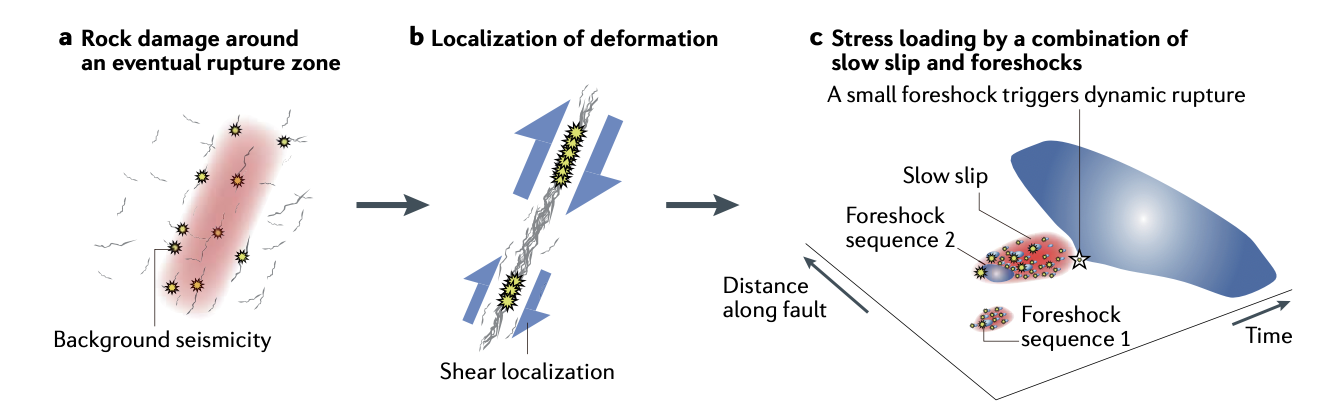
\includegraphics[width=\linewidth]{/Users/ntb3/Desktop/Grad_Project/Thesis_Figures,Images,Tables/generation_of_largequakes_concept_diagram.png}
		\caption{\textbf{Schematic illustrations of generation processes of large earthquakes.} \textbf{a} Progressive localization of shear deformation and background seismicity around a large rupture zone. \textbf{b} Shear localization and several foreshock sequences before the instability leading to the large rupture. \textbf{c} A space–time diagram of step-like increase in fault slip before a major earthquake associated with combined slow slip and foreshocks. A final rapid local loading by a small foreshock triggers the subsequent major dynamic rupture and circumvents the large nucleation process of a large patch. White and yellow stars denote epicentres of mainshocks and other events, respectively. As an example, two foreshock sequences accompanied with slow slip are displayed. (Kato, Ben-Zion, 2021)}
		\label{fig:generation_concept}
	\end{figure}
	
	
	
	
	\subsection{Earthquake Clustering}
	A basic characteristic of seismicity is earthquake clustering. Clustering is observed most clearly as the concentration and frequency of earthquakes around large faults and tectonic plate boundaries and after large earthquakes. Understanding seismic clustering plays an important role in many elements of seismicity, such as identifying the characteristics and interactions of active fault structures. 
	
	
	\subsubsection{Classification and Characteristics of Earthquake Clusters}
	
	Earthquake clustering is an important aspect of seismic activity that reveals valuable information about earthquake behavior. Clustering occurs in space, time, and size (such as magnitude and energy), and is the primary form of seismic activity. Spatial clustering appears as concentrations of earthquakes along major tectonic plate boundaries and regional fault networks, while temporal clustering involves increased seismic activity following large earthquakes, leading to aftershock sequences. However, there is no formal definition of seismic clusters, which hinders systematic global analysis. This section reviews the development of an objective and reliable method for analyzing seismic clusters.
	
	Mathematically, earthquake clustering is the separation of seismicity into groups that are closer in space and time than would be expected in a distribution that is completely random. These clustered groups of earthquakes reflect various triggering mechanisms, swarms and other forms of clustering as well as the traditional aftershock series. 
	
	A preliminary investigation of seismic clustering in southern California, detailed in the following section, revealed that clustering is strongly influenced by the crust's physical characteristics, leading to two primary types of clusters: "burst-like" and "swarm-like." These findings demonstrate the importance of region-specific factors in understanding earthquake dynamics and improving seismic hazard assessments. While high-quality data for southern California made these trends apparent, global data suffers from lower quality catalogs with increasing magnitudes of completeness/reporting and location uncertainty, affecting cluster characterization.
	
	In "A global classification and characterization of earthquake clusters", Zaliapin and Ben-Zion (2016) develop statistical tools for working with low-quality catalogs that are not sensitive to catalog inaccuracies. Zaliapin and Ben-Zion reveal that a main driving factor behind the types of clustering seen in a region is the effective viscosity of the region. Regions with increased effective viscosity experience burst-like clusters and regions with decreased effective viscosity experience swarm-like clusters. They show that local heat flow is the primary factor controlling the significant spatial dependencies of global earthquake clustering. 
	%Two primary categories of earthquake clusters—burst-like and swarm-like—are established. 
	Burst-like clusters are typical of cold places (mostly shallow seismicity of subduction zones), whereas swarm-like clustering is typical of hot regions (mainly mid-oceanic ridges). It is also shown that the sort of plate-boundary deformation only has a little impact on the seismicity cluster style. The global findings summarized below are consistent with previous regional findings based on higher-quality data in southern California and these results are found to be resilient to the known catalog uncertainties and inadequacies.
	
	
	
	% The below two paragraphs are first drafts of the above paragraph. These paragraphs have been moved to the section on the southern ca paper. 

	% Data and Methods 
	% Earthquakes 
	The authors used a global earthquake catalogue produced by the Northern California Earthquake Data Center (NCEDC) for the period of 1975 to 2015, containing 256,993 events. They used a minimum magnitude of 4, which is higher than the completeness magnitude in some regions but their analysis technique is still robust. 
	%They only considered earthquakes with depth less than 70 km, due to the uncertainty in depth reporting in the NCEDC catalogue. The spatial intensity of earthquakes, their maximum observed magnitude, and hypocentral depth show significant variations, as well as the catalogue's completeness. These variations were taken into account in the analysis to ensure robust results that reflect the regional cluster style.
	
	%heat flow
	Heat flow data from a study by Bird et al. (2008) was used to map the heat flow within seismically active areas and over the entire Earth surface. The highest heat flow production, reaching $0.3 W m^{-2}$, is found along the oceanic spreading ridges. 
	
	% Strain rate tensor
	The global strain rate field data from Kreemer et al. (2014) was used to study the deformation of the Earth's surface. The analysis is based on the second invariant of the strain rate tensor ($I_2$) and the tensor style ($S$) defined by Kreemer et al. The tensor style is used to classify the type of displacement into contraction ($S < -0.5$), strike-slip ($0.5 < S < -0.5$), and extension ($S > 0.5$).

	
	The minimum magnitude cutoff, $m_c$, in a catalog can affect aftershock analysis as earthquakes below this cutoff cannot be considered aftershocks of larger ones. A $\Delta$-analysis, which only considers mainshocks with a magnitude of at least $m_c+\Delta$ (in this case, $4$) and aftershocks $2$ units below the mainshock magnitude, is used to compare aftershocks of mainshocks with different magnitudes. Aftershocks found through this method are called $\Delta$-aftershocks and differ from regular analysis that considers all events.
	
	To understand earthquake clustering first consider generalized earthquake distance. When working with a catalogue where each event $i$ is characterized by its occurrence time $t_i$, hypocentre $(\phi_l, \lambda_i, d_i)$, and magnitude $m_i$, Baiesi $\&$ Paczuski (2004) define the proximity $ \eta_{ij}$ of earthquake $j$ to earthquake $i$ as:
	
	\begin{equation} \label{eq:generalized_distance}
	\eta_{ij} = \begin{cases}
		t_{ij}(r_{ij})^d10^{-bm_i}, & t_{ij}>0.\\
		\infty , & t_{ij} \leq 0.
	\end{cases}
	\end{equation}

	\noindent The event intercurrence time, $t_{ij}=t_{j}-t_{i}$, is positive if event $i$ occurs before event $j$; the spatial distance between earthquake hypo-centers is $r_{ij}\geq0$, the (possibly fractal) dimension of the hypo-centers or epicenters is $d$, and $b$ is the parameter of the Gutenberg–Richter law. Zaliapin $\&$ Ben-Zion (2013a, 2015, 2016a) address this proximity measure's justification and characteristics. 
	
	%One intuitive element of earthquake distance is that the proximity of one earthquake to it's nearest neighbor is inversely related to the seismic intensity. For high intensity processes where a larger number of events occur in the same space-time volume, the distance between events is smaller. 
	
	In identifying and characterizing earthquake clusters, it is necessary to identify the parent and offspring earthquakes in a catalog. To determine the distinct nearest neighbor(parent) $j$ for each event $i$ use the distance determined by (\ref{eq:generalized_distance}), and indicate this distance by the same symbol, $\eta_{ij}$. For this definition, event $i$ is referred to as an offspring of $j$, each event has a unique parent, aside from the first one in the catalog, and each parent might have multiple offspring.  
	
	\begin{figure}
		\centering
		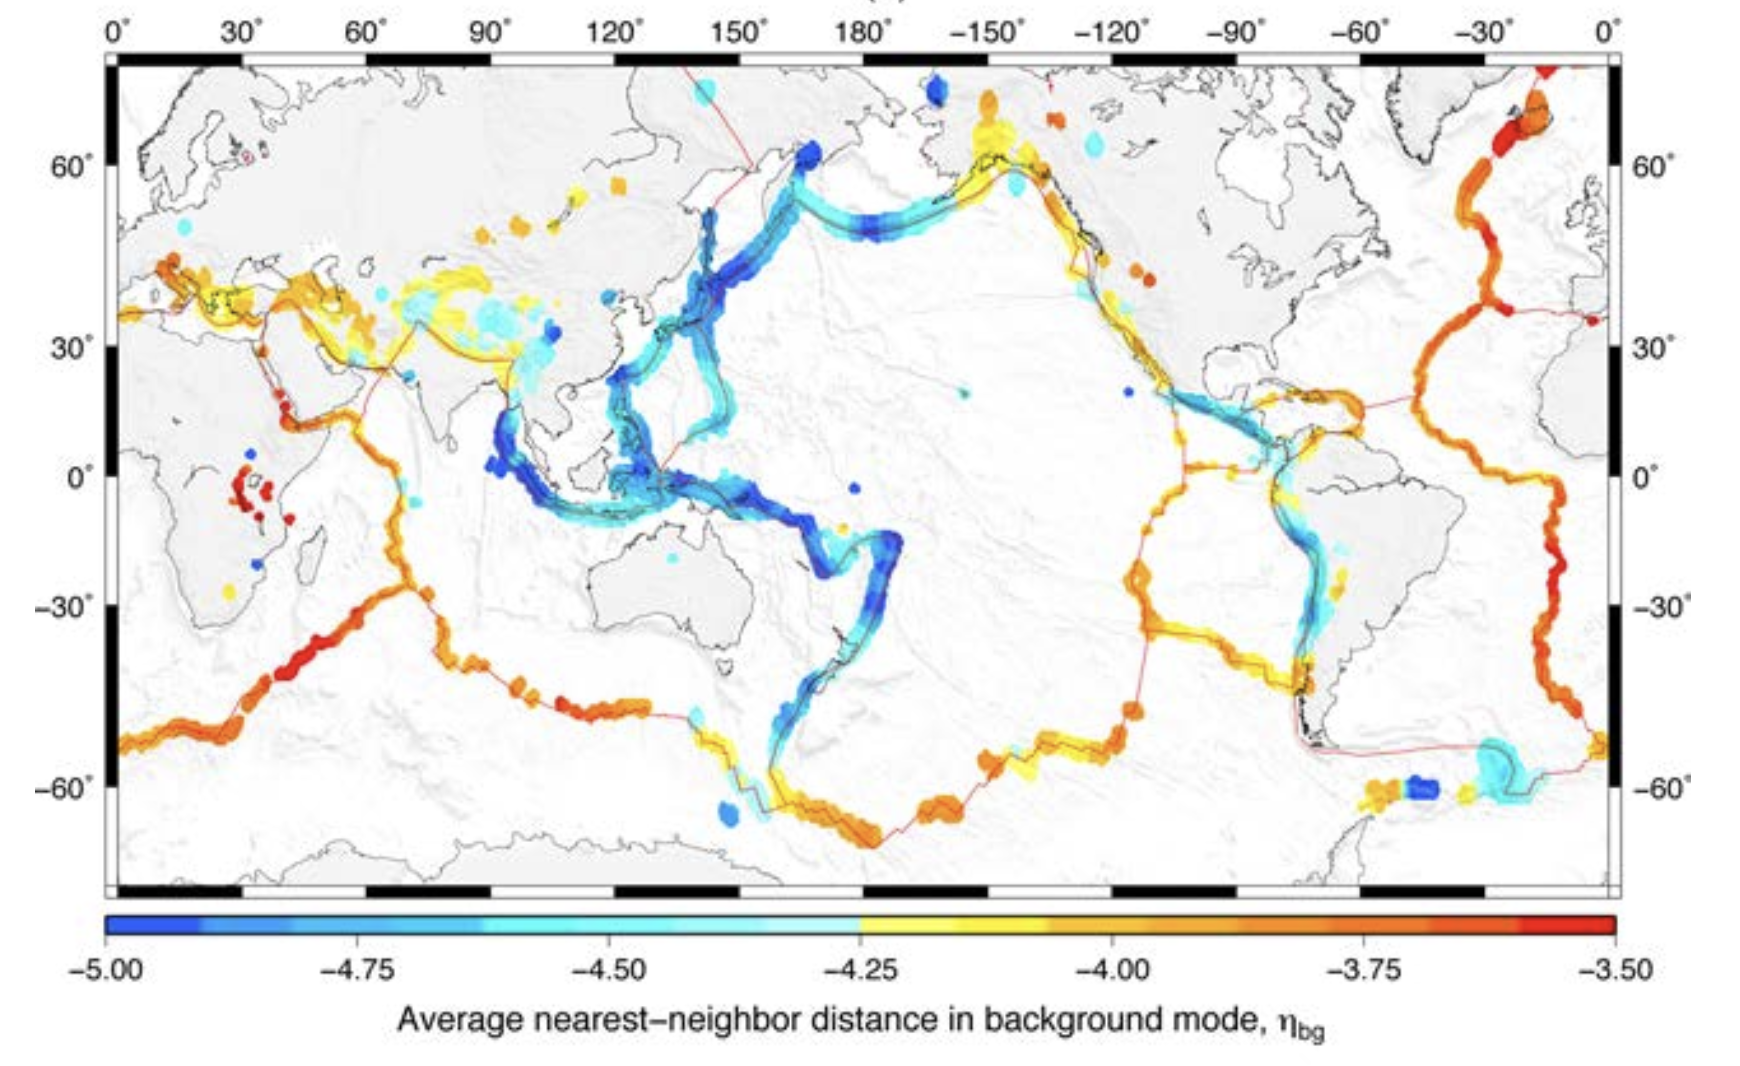
\includegraphics[width=0.9\linewidth]{Thesis_Figures,Images,Tables/average_nearest_neighbor_distance}
		\caption[Global maps of selected parameters of seismic clustering.]{Global maps of selected parameters of seismic clustering. Average nearest-neighbour distance $log_{10}\eta_{bg}$ in the background mode. (Zaliapin and Ben-Zion, 2016)}
		\label{fig:averagenearestneighbordistance}
	\end{figure}
	
	
	Zaliapin $\&$ Ben-Zion (2016a) have shown that the distance to the nearest-neighbor is distributed bimodally. The distance in space and time normalized by magnitude of the parent between a parent event $j$ and its offspring event $i$ is given by the formula
	
	
	\begin{equation} \label{eq:generalized_distance}
		T_{ij} = t_{ij}10^{-qbm_i};  R_{ij}= (r_{ij})^d10^{-pbm_i}; q+p=1
	\end{equation}
	
	\noindent as defined by Zaliapin et al. (2008). Theoretically, it can be shown that events with Gutenberg-Richter magnitudes and time-stationary space-inhomogeneous Poisson flow have a uni-modal distribution of $( \log T, \log R)$ concentrated along a line $\log_{10}T+ \log_{10}R = \text{constant}$. In reality, observed seismicity behaves differently. It has been established that detected seismicity over various regions has a bimodal joint distribution of $(\log_{10}T, \log_{10}R)$ where one of the modes coincides with background events and is comparable to the mode of a Poisson process. The other mode is made up of clustered events located noticeably closer in space and time to their parents than is likely in a Poisson process.
	
	\begin{figure}
		\centering
		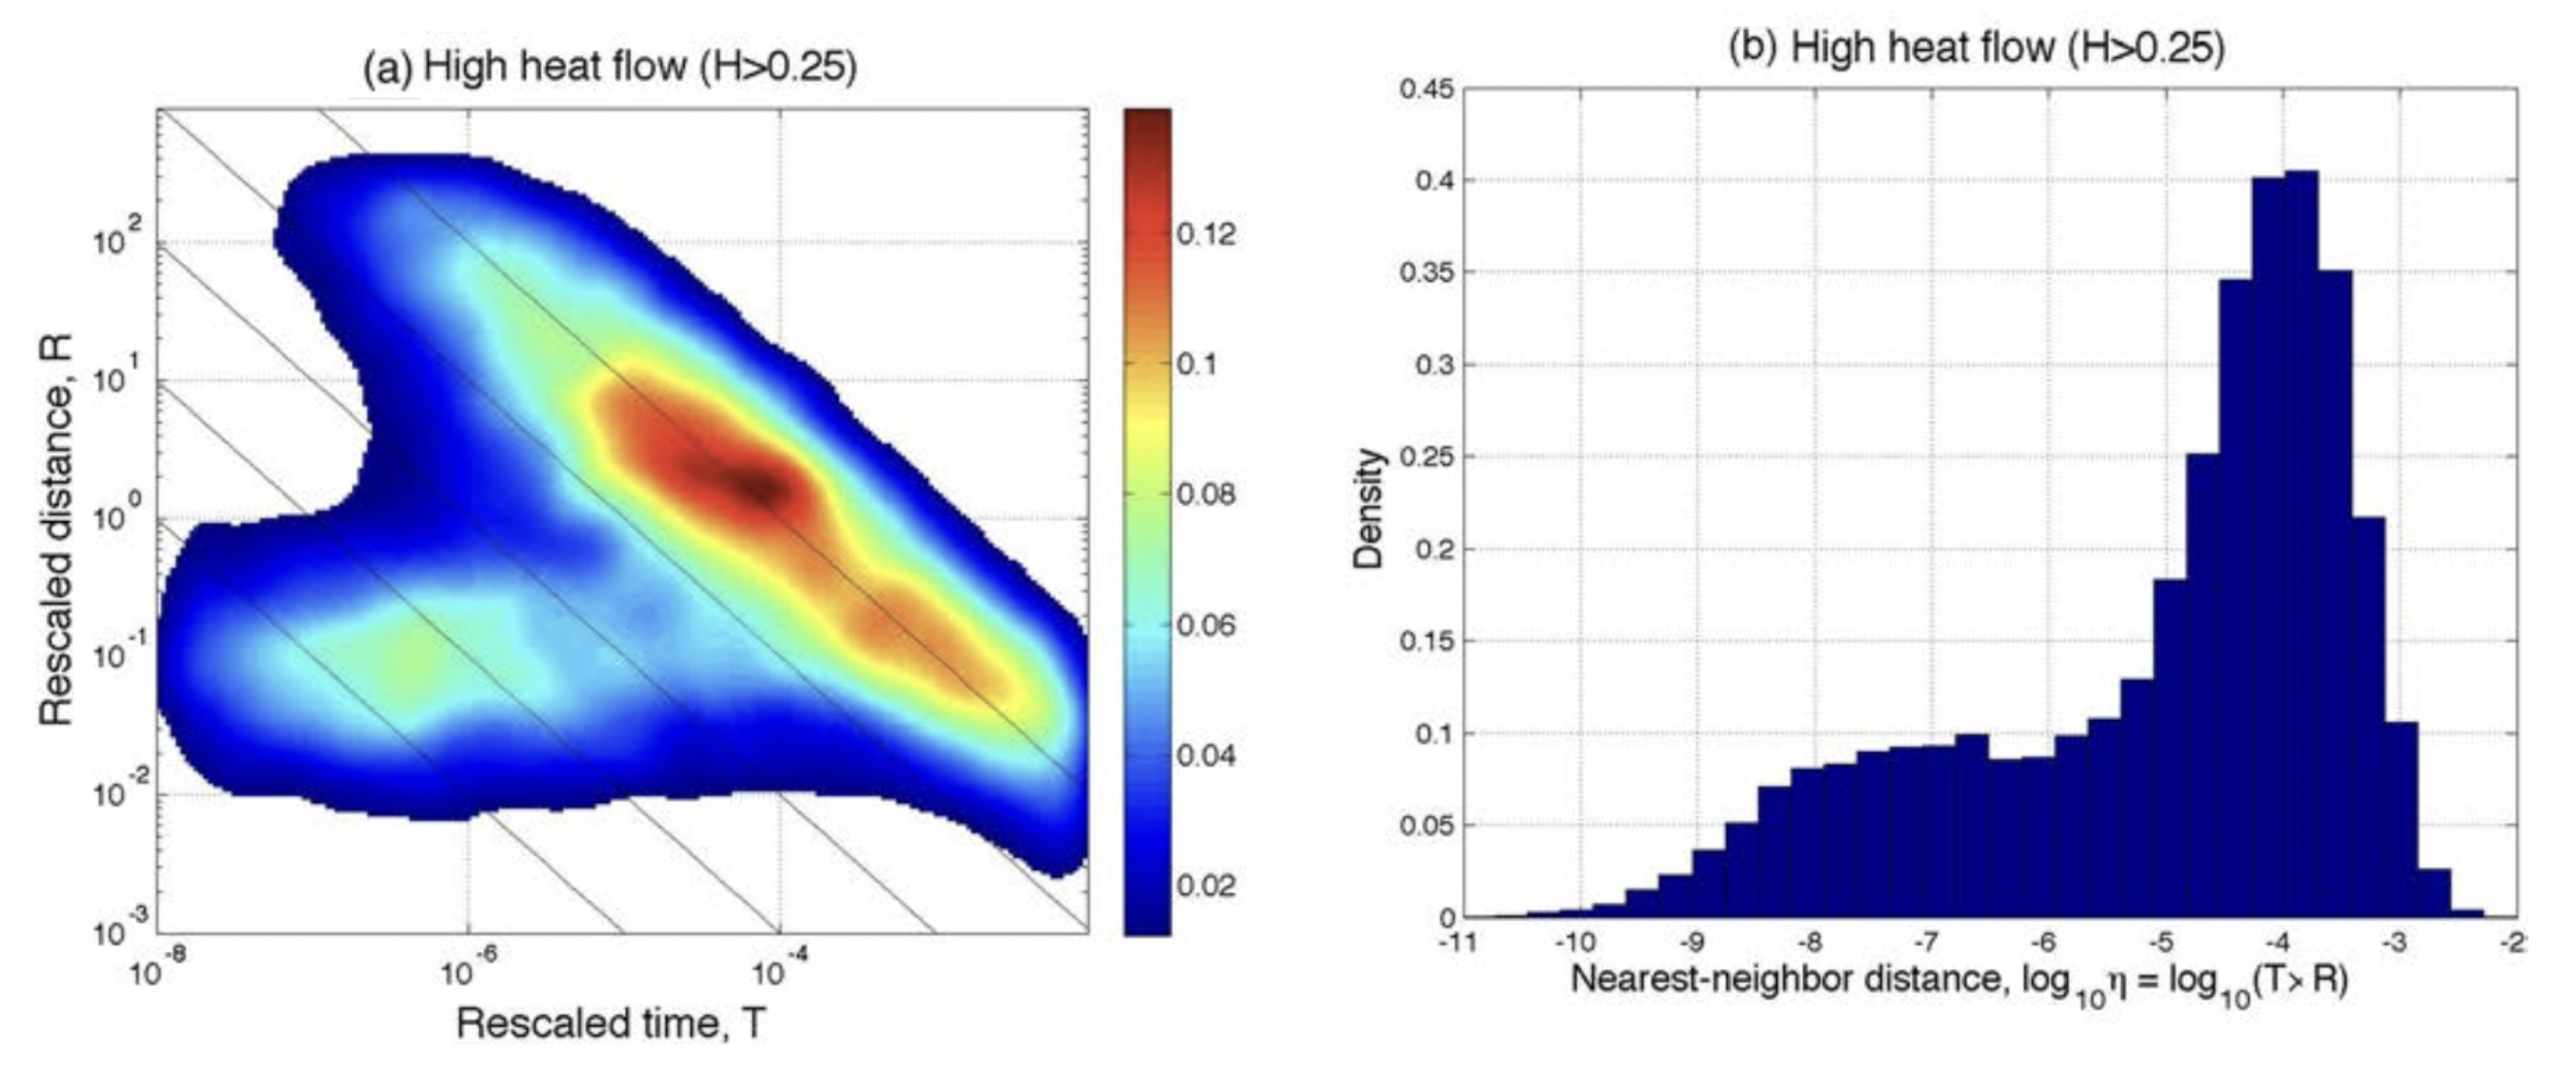
\includegraphics[width=0.8\linewidth]{/Users/ntb3/Desktop/Grad_Project/Thesis_Figures,Images,Tables/lit_review_bimodal.png}
		\caption[Bimodal distribution of generalized earthquake distance $\eta$.]{Generalized earthquake distance $\eta$ and its normalized space and time components $(T, R)$ in regions with high heat flow $H > 0.25$. (a) Joint distribution of the rescaled components $(T, R)$ of the earthquake nearest-neighbour distance. (b) Distribution of the values of the nearest-neighbour distance $\eta$. Black diagonal lines in panel (a) depict levels of constant distance $\eta$ (from top to bottom): $–\text{log}_{10} \eta = 4, 5, 6, 7, 8$. (Zaliapin \& Ben-Zion, 2016)}
		\label{fig:bimodal}
	\end{figure}
	
	\textcolor{blue}{How does this figure work for an example of a bimodal distribution?}
	
	
	A Gaussian mixture model approach can be used to distinguish the background and cluster modes in the bimodal distribution of earthquake distances. A Gaussian mixture model with two modes is used to intentionally select a nearest neighbor threshold $\eta_0$, so each event can be group into either the background (if $\eta_{ij}>\eta_0$) or cluster (if $\eta_{ij} < \eta_0$) mode.
	
	
	The distribution for a two mode Gaussian mixture model assuming that sample $x_i \in R^m, i=1,...,n$ is
	
	\begin{equation} \label{eq:gaussian_mixture_model}
	F(x) = wN(x; \mu_1, \Sigma_1)+(1-w)N(x; \mu_2, \Sigma_2).
	\end{equation}

	\noindent Here, $w$ is the mixture weight of the first mode and $N(x;\mu,\Sigma)$ denotes the Gaussian (Normal) distribution, with mean $\mu$ that is a vector with $m$ elements and variance $\Sigma$ that is a  $m \times m$ positive-definite matrix. Model estimation, mode and background (cluster) events threshold assignment are discussed in detail in Zaliapin $\&$ Ben-Zion (2016a). 
	
	From this model, two important parameters of clusters, $\eta_{bg}$ and $Q$, can be estimated for a region.  The mean generalized earthquake distance $\eta_{ij}$  of the background events from parent events is $\eta_{bg}$. The average value of the mode assignment probability $v = \max(w,1-w)$ over all events in a region is the regional mode separation quality $Q$. $Q$ can take on any value between $0.5$ and $1$. If each event can be classified as part of one of the modes with probability $1$ , $Q=1$, while if the classification of each event to either mode has probability $0.5$ then $Q = 0.5$. 
	
	%Clustering identification is done through the use of tree graphs and spanning forests. A spanning network representing a single cluster can be created by connecting each earthquake in a catalog to its nearest neighbor using the method above and produces a tree graph. Using the threshold $\eta \geq \eta_0$ to remove all links representing a large distance between parent and offspring creates a spanning forest. Each tree in the spanning forest represents a separate earthquake cluster. Some trees contain only single events ($\textit{singles}$) while others contain multiple events ($\textit{families}$).
	% the paragraoh below is a more concise version of the above paragraph
	Clustering identification is done using tree graphs and spanning forests. A spanning network representing a cluster is created by connecting each earthquake to its nearest neighbor, resulting in a tree graph. Applying a threshold $\eta \geq \eta_0$ removes links representing large distances between parent and offspring, resulting in a spanning forest where each tree represents a separate cluster. Trees may contain only single events ($\textit{singles}$) or multiple events ($\textit{families}$).
	
	%Within each family, the events are classified into $\textit{foreshocks}$, $\textit{main shock}$ and $\textit{aftershocks}$. The main shock is the earthquake with the largest magnitude in the family, and if multiple earthquakes have the same largest magnitude the first to occur is treated as the main shock. Foreshocks are the events proceeding the main shock and any events following the main shock are aftershocks. Each single is classified as a main shock. 
	% the paragraoh below is a more concise version of the above paragraph
	Events in each family are classified into $\textit{foreshocks}$, $\textit{main shock}$ and $\textit{aftershocks}$. The main shock is identified as the earthquake with the largest magnitude in the family, or the first to occur if there are multiple earthquakes with the same largest magnitude. Foreshocks are the events preceding the main shock, and aftershocks are the events following the main shock. Single events are classified as main shocks.
	
	% skipped over the parameters section here. 
	
	%Applying this method of analyzing earthquake clusters uncovered basic characteristics of sesimicity, features of the cluster and background modes and properties of earthquake clusters. The structure of earthquake families and the foreshock and aftershock sequences were also illuminated. 
	
	%ome key findings of basic characteristics of sesismicty uncovered include that earthquake clustering style is space-dependent and related to the heat flow production. The highest seismic activity typically occurred in subduction zones, and the average heat flow has the highest values exclusively within extension environments - particularly along the mid-oceanic spreading ridges. The space-dependent behavior of earthquake clustering is driven by the heat flow production. A few notable differences in the cluster style of earthquakes in high versus low heat flow regions are: (i) Higher earthquake intensity in low heat flow regions that have predominantly contraction and transform deformation style, (ii) the proportion of background events in low heat flow regions is lower than that in high heat flow regions(and the proportion of clustered events  is higher in low heat flow regions). (iii) The time decay of cluster events is faster in high heat flow regions, leading to stronger time separation between the background and cluster modes.
		% the paragraoh below is a more concise version of the above paragraph
	Earthquake clustering is space-dependent and related to heat flow production, with the highest seismic activity occurring in subduction zones and the average heat flow having the highest values in extension environments, particularly along mid-oceanic spreading ridges. The behavior of earthquake clustering is driven by space-dependent heat flow production. Notable differences in earthquake clustering between high and low heat flow regions include higher earthquake intensity in low heat flow regions with predominantly contraction and transform deformation styles, lower proportion of background events in low heat flow regions, and faster time decay of cluster events in high heat flow regions leading to stronger time separation between background and cluster modes
	
	A 1-D Gaussian mixture model applied to the nearest-neighbor distances of events within circles centered at the epicenters of all examined earthquakes was used to estimate the space-dependent threshold $\eta_0$ that separates the cluster and background modes. This threshold was then used to partition events into cluster and background populations. From this analysis properties of the cluster characteristics $\eta_{bg}$ and $Q$ were illuminated. The highest earthquake intensity and lowest values of $\eta_{bg}$ were observed within convergent environments, which flexibility large spatial variability and intermittence in separation quality $Q$. The lowest earthquake intensity and largest values of $\eta_{bg}$ were observed along divergent boundaries, and these boundaries also have high mode separation quality $Q$. Intermediate values of earthquake intensity and background position $\eta_{bg}$ were observed along transform boundaries, along with the mode separation quality Q showing high intermittency. A GLM approach and Spearman's correlation were used to compare earthquake cluster statistics with strain rate tensor and heat flow parameters. This approach further documented the correlation between heat flow and these examined cluster characteristics. 
	
	A key property of earthquakes clusters uncovered in this analysis was that cold areas have much larger clusters than hot areas. The study examines a catalogue of 256,993 events and partitions them into 135,840 clusters using a specific procedure. Of these clusters, 85.6$\%$ are single events and 14.4$\%$ are families with sizes ranging from 2 to 6584. The distribution of cluster size is found to be different in areas with high and low heat flow levels, with a power law tail approximation of 
	
	\begin{equation}
		S(N) = \sf Prob[\text{cluster size} > N] 	\propto N^{-\alpha} 
	\end{equation}
	
	
	\noindent with $\alpha \approx 2$ in hot areas and $\alpha \approx 1$ in cold areas. The observed difference in cluster size distributions implies that cold areas have much larger clusters and a larger proportion of clusters with size $N>10$. The dominance of large clusters in cold regions is explained by statistically higher maximal magnitude and better quality of catalogues in cold regions compared to hot ones. The cluster size is stochastically larger in cold regions for clusters with main shock magnitude $m>6$, while the size of intermediate-magnitude clusters (with main shock magnitude $m<6$) is stochastically larger in hot regions. In addition, the proportion of smallest clusters (singles) among all detected clusters is higher in cold areas. The probability of being a single is higher for small-magnitude events. With the existing data, it is difficult to conclude whether this effect is related to the inferior catalogue quality in hot regions or is a real physical property.
	
	%Same as two bellow
	The proportion of foreshocks among foreshocks and aftershocks, $p_F$, is higher in areas with high heat flow, typically with values greater than $0.2$, while in areas with low heat flow the typical proportion is very small, $p_F<0.1$. This increased production of foreshocks in hot regions is supported by the analysis of the value of $p_F$ averaged for different combinations of strain rate tensor's style $S$ and second invariant $I_2$. Spatial patterns similar to those reported in \ref{fig:proportionofforeshocksamongaftershocks} are also seen for other examined cluster characteristics. 
	When looking at the worldwide distribution of the aftershock magnitude gap $\Delta A$ defined for families with aftershocks as the difference between the magnitudes of the main shock and the largest aftershock, this gap is generally larger within cold regions, with typical value of $\Delta A \approx 0.8$, while in hot regions it is typically smaller, $\Delta A \approx 0.55$. The comparison of $p_F$ and $\Delta A$ with heat flow and strain rate tensor parameters using Spearman's correlation and GLM approach, it is notable that the values of the aftershock magnitude gap reported here are lower than the value $\Delta A \approx 1$ suggested by the Bath law. This deflation is artificial and is due to the fact that we consider families with main shock magnitude $m \geq 5$, which is only one unit above the magnitude cut-off $m_{min} = 4$ selected for this study. The magnitude gap is affected by the catalogue completeness magnitude, since a higher completeness magnitude leads to smaller observed values of $\Delta A$. The reported difference in magnitude gap might be influenced to some extent by inferior catalogue quality in hot areas. However, Zaliapin $\&$ Ben-Zion reported lower magnitude gap in hot regions in a local study in southern California, where the quality of catalogues is comparable in both cold and hot regions. The study believes that the magnitude gap difference between hot and cold areas is a real phenomenon that will be confirmed in future studies with better catalogue quality.
	
	\begin{figure}
		\centering
		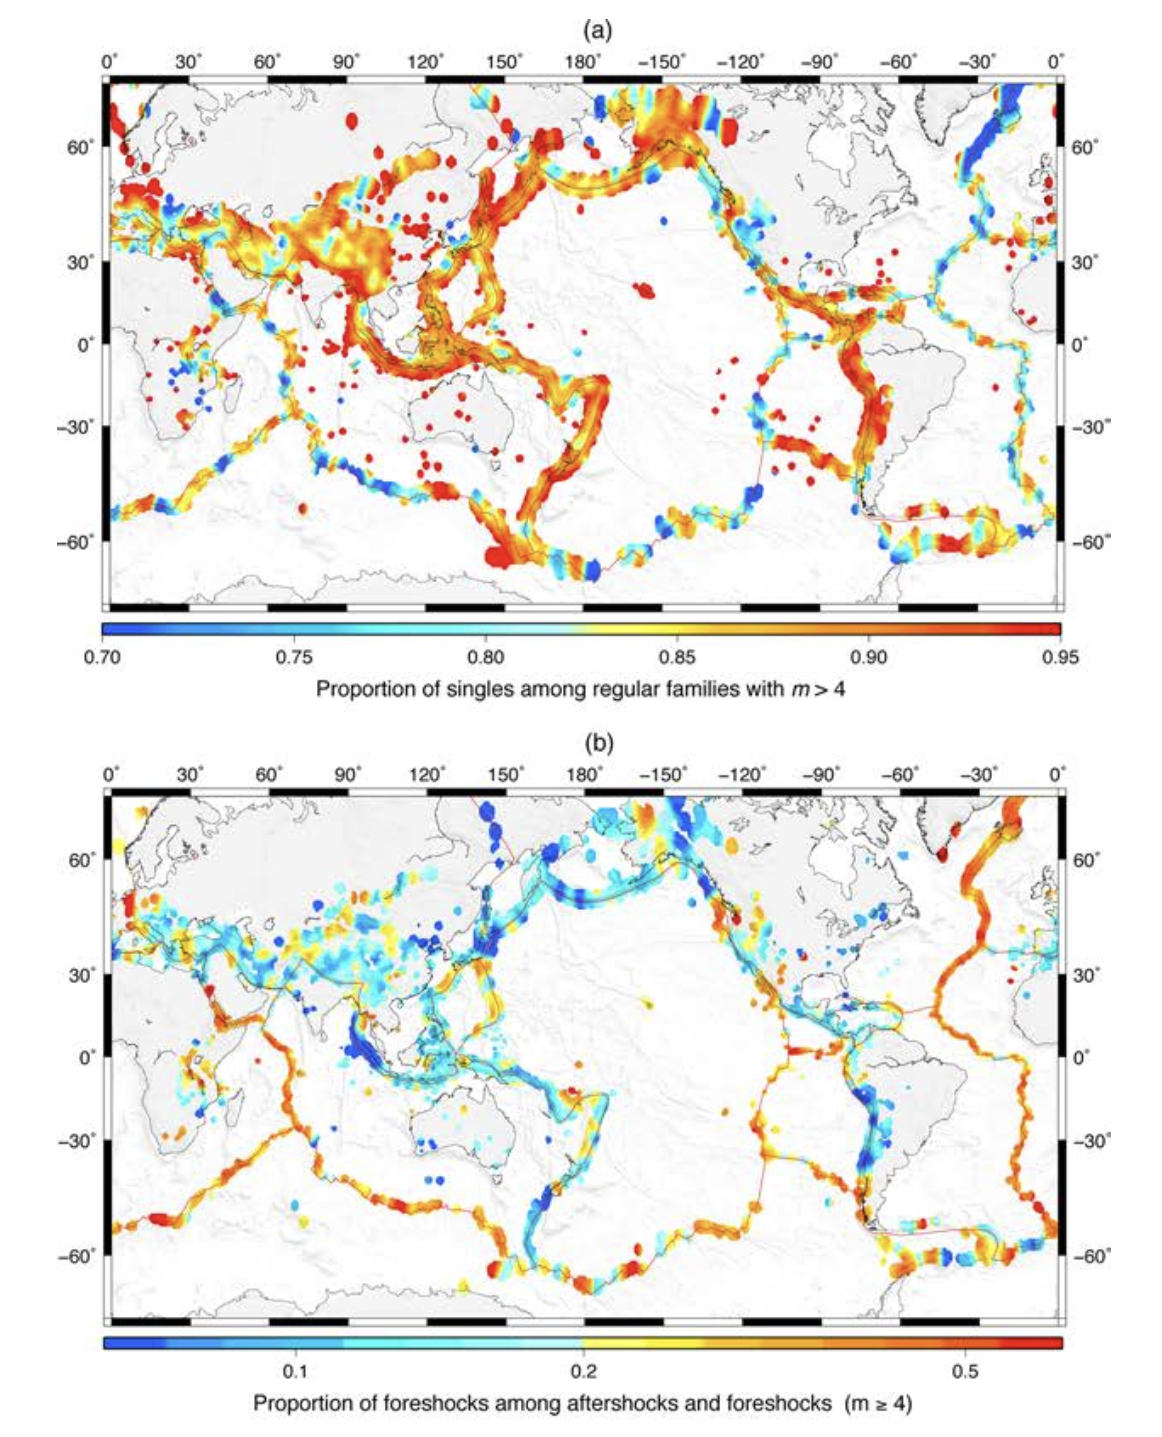
\includegraphics[width=0.9\linewidth]{Thesis_Figures,Images,Tables/proportion_of_foreshocks_among_aftershocks}
		\caption{Global spatial distribution of selected earthquake cluster statistics. (a) Proportion $p_S$ of singles among regular clusters. (b) Proportion $p_F$ of foreshocks among foreshocks and aftershocks. (Zaliapin and Ben-Zion, 2016)}
		\label{fig:proportionofforeshocksamongaftershocks}
	\end{figure}
	
	
	As mentioned previously, the structure of earthquake families is represented by a tree, $T$, with vertices, $V={v_i}, i = 1,...,N$ representing earthquakes and edges, ${e_i}$ connecting them to their parent within the same family. The first event in the family is referred to as the root and all other events have a single parent within the same family. Two statistics are used to study the structure of earthquake families: the average family branching and the average leaf depth. The average family branching is the average number of offspring per parental vertex of the tree, while the average leaf depth is the average number of edges between a leaf and the tree root. It is expected that the leaf depth and family branching are negatively correlated, meaning that as the leaf depth increases, the family branching decreases. Zaliapin and Ben-Zion (2013b) found that these statistics are strongly coupled with the heat flow in southern California, with leaf depth increasing and family branching decreasing as heat flow increases. The same trend is observed on a global scale. The values of these statistics also depend on the family size, which can affect spatial analysis. A least-square regression analysis suggests that the examined statistics have a relation to the family size in the intermediate size range of 5 to 20. The spatial distribution of these statistics also shows that cold regions typically have a smaller average leaf depth and a larger average family branching than hot regions. The comparison of these statistics with heat flow and strain rate tensor parameters using Spearman's correlation and GLM approach confirms that heat flow exerts the primary control on the values of these two statistics.
	
	%This study examines the existence of universal laws in earthquake dynamics on a global scale and supports earlier findings that there is non-universal, region-specific behavior of seismicity by extending the analysis of earthquake clusters in southern California to a global scale using data from the NCEDC worldwide catalog for the period 1975-2015. The study uses a nearest-neighbor approach to partition the earthquakes reported in the NCEDC global catalog into individual clusters, and then compares the worldwide space distribution of various cluster statistics with global heat flow production and style of lithospheric deformation indicated by an estimated strain rate tensor. The study found that multiple statistics of earthquakes and seismicity clusters have spatially dependent distribution, tightly correlated with the global heat flow production. The results are consistent with those obtained in a local analysis of southern California, and with theoretical expectations based on a viscoelastic damage rheology model. The overall picture emerging from these studies indicate that there exist two primary types of earthquake clustering. In cold regions, brittle fracture results in burst-like clusters characterized by a prominently large main shock that happens in the very beginning of the sequence and triggers multiple offspring of smaller magnitude occurring in a small number of generations and decaying until merging with the background seismicity. In contrast, in warm regions, the seismicity is more diffuse and characterized by a smaller main shock and a larger number of offspring events.
		% below is a short version of above
	This study investigates earthquake dynamics on a global scale and found that earthquake statistics and cluster characteristics have a spatially dependent distribution, which correlates with global heat flow production and style of lithospheric deformation indicated by an estimated strain rate tensor. The results support earlier findings that there is non-universal, region-specific behavior of seismicity, and suggest that there are two primary types of earthquake clustering: burst-like clusters characterized by a large main shock in cold regions, and diffuse clusters with a smaller main shock and a larger number of offspring events in warm regions. The findings are consistent with theoretical expectations based on a viscoelastic damage rheology model.
	
	\subsection{Applications - Earthquake clusters in southern California }
	
	\subsubsection{Identification and stability}
	
	% Introduction Summary
	
 	This section explores the application of the techniques discussed in the previous section to identify and characterize the clustering of seismicity in southern California. The study "Earthquake clusters in southern California I: Identification and stability" by Zaliapin and Ben-Zion (2013)  uses the method based on the bimodal distribution of nearest-neighbor earthquake distances in a combined space-time-magnitude domain, which allows for partitioning an earthquake catalog into separate individual clusters mentioned in the previous section. The clusters are divided into singles, which contain just one event, and families, which contain multiple events, and are subclassified into foreshocks, mainshocks, and aftershocks. Recall this method is characterized by its ability to use only three easily estimated parameters, its ability to uniformly analyze clusters associated with mainshocks of greatly different magnitude, its high stability with respect to parameters, minimal reported magnitude, catalog incompleteness, and location errors, and its absence of underlying assumptions or governing models for the expected earthquake cluster structure.
		
	%Data and Basic Methods Summary
	The study uses a the by Hauksson et al. (2012) catalog. Figure \ref{fig:socalseismicity} in the study shows the location of these earthquakes and Figure \ref{fig:observedseismicity} provides a visual representation of changes in seismic intensity, which are mostly related to aftershocks of large earthquakes.
	
	\begin{figure}[t]
		\centering
		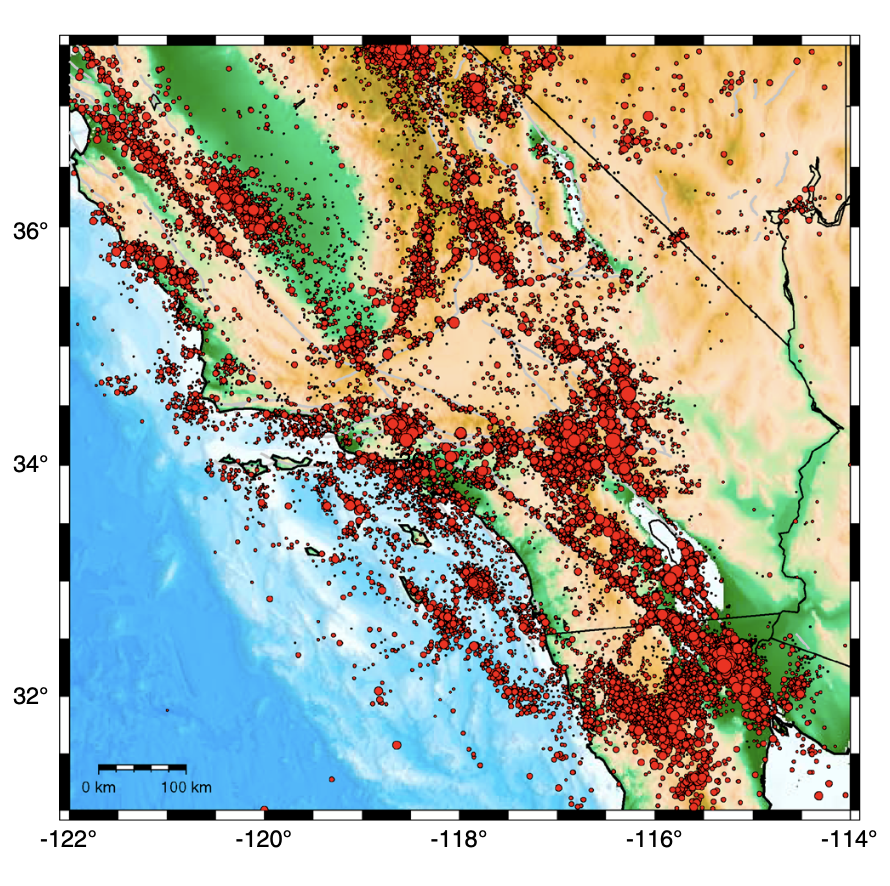
\includegraphics[width=0.7\linewidth]{Thesis_Figures,Images,Tables/socal_seismicity}
		\caption{Map of earthquake epicenters, $m \geq 2$, from the relocated catalog of Hauksson et al. [2012]. Circle size is proportional to magnitude. Major faults are shown by gray lines.}
		\label{fig:socalseismicity}
	\end{figure}
	
	
	\begin{figure}[b]
		\centering
		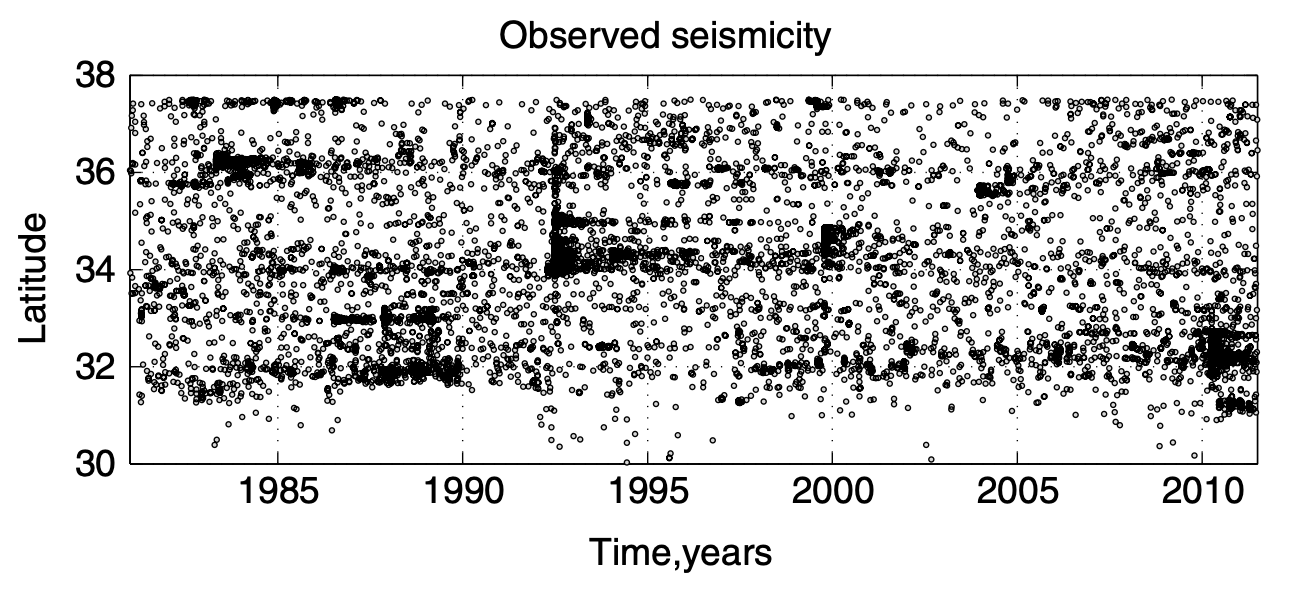
\includegraphics[width=0.7\linewidth]{Thesis_Figures,Images,Tables/observed_seismicity}
		\caption{Epicenters of the earthquakes with $m \geq 3$ as a function of time and latitude.}
		\label{fig:observedseismicity}
	\end{figure}
	
	
	%Magnitude of completeness
	Despite using a lower completeness magnitude of $m_c=2$ compared to the estimated completeness magnitude of 3.0 for southern California, the study found that the cluster structure of events is unaffected by incompleteness or the minimum reported magnitude. This indicates that the recovered cluster structure is similar to what would be observed in a complete catalog. Results for a higher magnitude threshold of 3 are similar, but there are insufficient clusters to obtain clear results.
	
	% delta analysis covered in previous seciton
	
	
	%Earthquake clustering and nearest neighbor approach and distance between earthquakes
	In this study, earthquake clusters are identified by the nearest neighbor approach discussed in detail in the previous section. The analysis shows two distinct groups: clustered events that are close to each other in time and space, and background events that are farther apart than expected. Although background events are not entirely homogeneous, deviations are smaller than for clustered events. The study focuses on significant clusters, their properties, and the single largest event in each cluster, regardless of homogeneity. This approach differs from catalog declustering, which removes events to create a homogeneous set. Recent research shows that the assumption of catalog homogeneity is often incorrect due to seismic migration and changes in activity.
	
	%Homogeneour poisson process
	Results from analyzing 2,105 events with $m \geq 3$ in southern California, using the Hauksson et al. relocated catalog, suggest that they form a Stationary Homogeneous Poisson (SHP) process. This process is a marked Poisson point process that is uniform across multiple dimensions, stationary over time, and has magnitudes that follow the Gutenberg-Richter distribution. The joint 2-D distribution of time and distance in SHP is unimodal and concentrated along the line $\log_{10}T+\log_{10}R=-5$, as shown by exploring Nearest Neighbor distances (NND). A histogram of NND on a logarithmic scale also displays a clear unimodal shape in the joint distribution of time and distance of the SHP process, which closely matches the theoretical Weibull distribution. This aligns with the analysis outlined in the previous section.
	
	%observed seismicity
	Observed seismicity in Southern California uncovers a prominent bimodal distribution of $\eta$ and of the joint distribution of $(T,R)$. The first mode, referred to as the "background," is similar to the distribution of a SHP process. The second mode, referred to as "clustered," is located closer to the origin. This bimodal distribution has also been observed in global seismicity and regional seismicity in other areas such as Nevada, Japan, New Zealand, and Africa. The bimodal distribution is caused by groups of earthquakes happening within localized regions in space and time, mainly corresponding to foreshock-mainshock-aftershock sequences or swarms. The bimodality of the $(T,R)$ distribution is used to identify individual space-time clusters of seismicity.
	
	%Spanning Network, Forest of Earthquakes
	A nearest-neighbor spanning network from the southern Califonria earthquake catalog was created by connect each earthquake to its closest neighbor to form a single cluster that includes all earthquakes. This nearest-neighbor network is a tree structure without loops. The links in the tree are then separated into strong and weak links based on their proximity, NND $\eta$. Weak links correspond to the background part of the bimodal distribution of seismicity, while strong links correspond to the clustered part of the bimodal distribution. The weak links are removed to form a spanning forest, which is made up of a collection of distinct trees, which includes single-event trees (singles) and multievent clusters (families) as discussed in the previous section. $60\%$ of the earthquakes have strong links and form families, while $40\%$ have weak links and are singles in the southern California catalog. If we zoom in on a specific aftershock sequence we can see the highly clustered nature of families of events, while singles are more uniformly distributed. 
	
	%Mainshocks, Aftershocks, Foreshocks
	When examining the internal composition of the clusters within the nearest-neighbor spanning forest, families, are separated into "mainshocks," "aftershocks," and "foreshocks." The type of earthquake depends on the time and magnitude. The analysis shows that the proportion of different types of earthquakes is stable for families with magnitudes below 5, with about $37\%$ of mainshocks and singles, $56\%$ aftershocks, and $7\%$ foreshocks.  For larger earthquakes, there is a preference for mainshocks. The spatial and temporal distribution of mainshocks and singles is larger than that of the clusters identified by the nearest-neighbor analysis. The mainshock/single field is not Poissonian and the cluster identification procedure does not distort the nonhomogeneous and possibly nonstationary background events. However, the clustering of mainshocks and singles lacks bimodality, so additional rules are required to analyze such data.
	
	%Quality and Stability of Cluster Identification
	The technique for detecting earthquake clusters used in this study is based on the earthquake distance equation (Equation \ref{eq:generalized_distance}) and a cluster threshold $\eta_0$ as described in the previous section. The technique is completely parameterized by three values $(b, d_f, \text{and} \eta_0)$ that are estimated from observations. The performance and stability of the technique were tested using catalogs generated by the ETAS model. The results suggest that the technique can accurately identify clusters in the ETAS model, is stable with respect to various parameters, and can be applied to the observed catalog of southern California seismicity. The study uses a version of the ETAS model that assumes isotropic spatial kernel and homogeneous spatial background, which is commonly used in seismicity analysis. The results suggest that the cluster structure in the southern California catalog is similar to that generated by the ETAS model, and the proposed technique can robustly recover the cluster structure.
	
	% Statistics of Detected Clusters
	When analyzing the statistics of the detected earthquake clusters, Zaliapin and Ben-Zion had two objectives. The first objective was to validate the proposed cluster detection technique by reproducing known statistical features of aftershocks and foreshocks. The second objective was to uncover new properties of the earthquake clusters.
	
	% Magnitude Distibution 
	
	When looking at the magnitude distributions of mainshocks/singles, aftershocks, and foreshocks, the cumulative proportion of earthquakes above or equal to magnitude $m$ is normalized by the magnitude, $[1-F(m)]x10^m$ where $F(m)$ represents the empirical cumulative distribution function of magnitudes, to emphasize the changes in the exponential index. This transformation shows that all three distributions are exponential within the magnitude range of 2.5 to 4.5, with a lower index, $b \approx 1 $, for mainshocks and aftershocks and a higher index, $b>1$ for foreshocks. The estimation of the b-value, which is a measure of the rate of earthquakes, confirms the visual observations from the cumulative plots of observed seismicity. The b-value for mainshocks and aftershocks is the same, while it is higher for foreshocks. The mainshock/single magnitude distribution does show an upward deviation from the exponential distribution and it is thought this is due to growth of stress concentration in elastic solid with rupture size, but the exact reason remains unclear, and may be due to either statistical artifacts or physical processes. The results suggest that the behavior of natural seismicity clusters and foreshocks, in particular, cannot be fully explained by the ETAS framework.
	
	% number of offspring
	When the number of offspring events $(N_{\text{off}})$ in a catalog of observed earthquakes is compared to an ETAS model catalog, the results showed that the $N_{\text{off}}$ distribution for fixed $m$ in the observed catalog deviates significantly from a Poisson distribution and is better approximated by a negative binomial distribution, which is consistent with previous research. 
	
	For observed seismicity in southern California, the offspring number scales with the event magnitude as 
	
	\begin{equation} \label{eq:offspring_number_soCal}
		N_{off}\propto 10^{cm},c = 0.93\pm 0.06
	\end{equation}
	
	
	\noindent where the estimation is done within the range $4 \leq m \leq6$, and at the $95\%$ confidence level. 
	
	The estimated mean and variance of $N_{off}$ for the observed catalog is larger compared to the ETAS model. In particular, the average $N_{off}$ for earthquakes with magnitude less than 4 is significantly smaller in the ETAS model than in the observed catalog. The ratio between the variance and average also increases from 1 to about 100 as the magnitude of earthquakes increases from 2 to 6 in both the observed catalog and ETAS model, further emphasizing the inadequacy of the Poisson model for describing the $N_{off}$ distribution.
	
	An important result of this increased variability of the $N_{off}$ distribution in the observed catalog is the existence of a large population of "singles" or main shocks with no offspring. This observation cannot be solely explained by catalog artifacts such as incompleteness or the minimal reported magnitudes. Singles make up $84\%$ of all detected clusters, $53\%$ of clusters with magnitude greater than or equal to 3, and $17\%$ of clusters with magnitude greater than or equal to 4. The largest single event detected has a magnitude of 5.0.
	
	%Cluster Size, Number of Foreshocks, Aftershocks
	The distribution of cluster size $N$ is found to be closely approximated by a Pareto distribution with a index $a \approx -1$, which can be explained by the combination of exponential mainshock magnitude distribution and the exponential number of offspring for a given mainshock with index $\alpha \approx b$. The number of aftershocks per cluster is larger and scales with the mainshock magnitude as $N_A \propto 10^{\beta m}$ with an index of $\beta \approx 0.99 \pm 0.06(95\% CI)$. The number of foreshocks doesn't exhibit a clear exponential scaling but the best exponential fit would have a smaller index of $\beta \approx 0.6$. The increase of fore/aftershock number with the cluster mainshock magnitude is due to the existence of the catalog lower cutoff magnitude. The cluster size is found to be independent of the mainshock magnitude and robust with respect to the earthquake magnitudes after conducting various tests.
	
	%Temporal Structure of Families
	To understand the temporal structure of families the intensity of earthquakes in the clusters versus time is averaged over all the detected clusters in both regular and $\Delta$-analyses, specifically looking at the relationship between the intensity and time relative to the main shock. Results from both regular and $\Delta$-analyses (which only includes aftershocks and foreshocks within $\Delta$ magnitude units from the main shock) showed a conventional pattern of foreshock-mainshock-aftershock, with lower number of foreshocks and higher number of aftershocks. The intensity of both aftershocks and foreshocks decreases over time, with a power-law decay seen in both. Results were consistent with the Omori-Utsu law (\ref{eq:ppintensity}) for the intensity of both foreshocks and aftershocks, and showed that the productivity index K is a constant dependent on $\Delta$ but not the main shock magnitude in $\Delta$-analysis, while in regular analysis it scales with the main shock magnitude $m$ as
	
	\begin{equation} \label{eq:K}
		K=10^{\beta m }
	\end{equation}

	\noindent with $\beta \approx 1$ for aftershocks and $\beta <1$ for foreshocks. The difference between the aftershock intensity in regular vs $\Delta$-analysis was significant, while the difference between the foreshock intensities was much smaller. This difference was seen in the distribution of magnitude differences between the main shock and the family events, with foreshocks having a closer magnitude to the main shock compared to aftershocks. However, the distributions of the magnitude difference between the main shock and the largest foreshock or aftershock were statistically the same. These results suggest the existence of an accelerated failure process as the time of main shock approaches.
	
	%Båth Law for Foreshocks and Aftershocks
	Previous research has shown a systematic difference between the magnitudes of mainshocks and their largest aftershocks with an average magnitude difference close to 1.2. The current analysis of southern California confirms this, with an average magnitude difference of 1.1 for aftershocks and 1.2 for foreshocks. The differences in magnitude, $\Delta_m = m_{\text{mainshock}}-m_{\text{largest-event}}$ are found to have an almost uniform distribution within the range of $[0, 2]$. However, the data shows significant deviations from a uniform distribution in the foreshock magnitude distribution in the ETAS model. Further testing is needed to determine if this deviation is systematic and if the ETAS model deviates from observations regarding foreshock magnitudes.
	
	%Area and Duration of Families
	%old version below next paragraph that begins with The size is the shrotened version.
	%The area of foreshock and aftershock sequences and the magnitude of the mainshock are related. The area $A$ of the groups of earthquakes is defined as the area of the smallest convex hull that contains them. The results showed that the area $A$ of aftershocks scales with the mainshock magnitude $m$ as $A \propto 10^{\gamma m}$, $\gamma \approx 1$ and is independent of the family size $N$. This suggests the presence of a damage zone around the parent rupture with a linear size that scales with the mainshock magnitude. The foreshock area, on average, was found to be an order of magnitude smaller than the aftershock area and independent of the family size. The duration of the family was also found to be independent of the mainshock magnitude and slightly increasing with the family size, indicating that the stress relaxation process after a mainshock is dominated by elastic stress transfer.

	The size of earthquake clusters relates to the main earthquake magnitude, with the area A defined as the smallest convex hull containing them. Aftershock areas scale with the mainshock magnitude $m$ as $A \propto 10^{\gamma m}$, $\gamma \approx 1$, and are independent of family size $N$, suggesting a damage zone around the main rupture that scales with its magnitude. Foreshock areas are an order of magnitude smaller on average than aftershock areas and independent of family size. Cluster duration is independent of main earthquake magnitude and slightly increases with family size, indicating elastic stress transfer dominates stress relaxation after a mainshock.
	
	%This paragraph and the next are made more concise in the following paragraph that starts with "Seismic clustering"
	%The clustering style of seismicity in southern California is strongly connected to the physical characteristics of the crust and is evolving at the scale of tens of kilometers. Two primary types of clusters exist in southern California, "burst-like clusters and "swarm-like clusters". "Burst-like clusters" have a distinct large main shock, few foreshocks, and larger number of first-generation offspring. In regions with cold crystalline rocks, decreased fluid content, and minimal heat flow output, these clusters represent a very brittle quick collapse process.  The Mojave, Ventura, and San Gabriel regions are some examples of areas in southern California that experience burst-like clusters. "Swarm-like clusters," are characterized by their lack of a noticeable primary shock. They have more foreshock activity than burst-like clusters and have a lot of secondary, tertiary, etc offspring. These clusters signify mixed brittle-ductile failure in regions of high fluid, heat, and/or soft sediment flow. The Salton Sea and Coso geothermal districts in southern California are examples of swarm-like cluster locations. A main driving factor behind the types of clustering seen in a region is the effective viscosity of the region. Regions with increased effective viscosity experience burst-like clusters and regions with decreased effective viscosity experience swarm-like clusters. 
	
	%These southern California results indicate the presence of region-specific factors that offer crucial information on earthquake dynamics and can improve seismic hazard assessments. The high quality data for the region of southern California is what makes it possible to uncover these trends. Unfortunately, the global data is not of the same quality.  Cluster characterization is affected by elements of lesser quality catalogs such as increasing magnitudes of completeness/reporting and earthquake location uncertainty. As discussed in the previous section in "A global classification and characterization of earthquake clusters", Zaliapin and Ben-Zion develop statistical tools for working with low-quality catalogs that are not sensitive to catalog inaccuracies.  
	
	Seismic clustering in southern California is tied to crustal properties and changes over tens of kilometers. Two primary types of clusters exist: "burst-like" and "swarm-like." Burst-like clusters have a distinct large main shock, few foreshocks, and more first-generation offspring, indicating brittle collapse in regions of low fluid and heat flow. The Mojave, Ventura, and San Gabriel regions have burst-like clusters. Swarm-like clusters lack a noticeable primary shock, have more foreshock activity, and many secondary offspring, indicating mixed brittle-ductile failure in regions of high fluid, heat, and/or soft sediment flow. The Salton Sea and Coso geothermal districts have swarm-like clusters. Effective viscosity is the primary driver, with increased viscosity leading to burst-like clusters and decreased viscosity leading to swarm-like clusters. These trends in southern California provide valuable insights into earthquake dynamics and seismic hazard assessments but are limited by the quality of global earthquake data, which can be improved using statistical tools developed by Zaliapin and Ben-Zion(2016) discussed in the previous section.
	
	
	\subsubsection{Spatial variations of Rock damage production} 
	
	%INTRODUCTION 
	%"Spatial variations of rock damage production by earthquakes in southern California" (Ben-Zion $\&$ Zaliapin, 2018) endevours to estimate the amount of rock damage produced by earthquakes in Southern California. The authors use data from earthquakes with magnitudes in the range $[2,4)$ from 1981 to 2017. The study aims to understand the relative production of rock damage in different parts of Southern California. The authors use theoretical relations from earthquake phenomenology and fracture mechanics to estimate the production of fracture area and volume generated by observed seismicity. The results of the study indicate that there is a zone with ongoing damage production between the Imperial fault and the Eastern California Shear Zone. The regions around the 1992 Joshua Tree, Landers and Big Bear earthquakes are active before 1990 and outline the future earthquakes. The seismicity and damage zone become more pronounced and continuous with increasing depth leading up to these larger events. Finally, implications of these results for the properties and dynamics of the plate-boundary region in Southern California are discussed.
	
	%Methodology 
	Estimating the amount of rock damage produced by earthquakes in southern California is done by using observed seismicity, basic relations from earthquake events and fracture mechanics. The authors provide theoretical formulations for calculating the fracture area and rupture volume, which are then implemented using the earthquake catalog for the period 1981-2017.
	
	% Fracture area 
	%The method for estimating the total fracture area and rupture volume associated with a population of earthquakes uses basic empirical relations of earthquakes and theoretical results from fracture mechanics. 
	The total number of earthquakes with a magnitude of M or greater is given by the Gutenberg-Richter exponential relation. The fracture area of each earthquake is estimated by assuming it can be approximated as a circular crack with a uniform strain drop in a solid. The seismic potency of each earthquake is related to its magnitude. By combining these relationships, the total fracture area is calculated by integrating the fracture area of each earthquake. The calculation shows that the smallest earthquakes in the population dominate the total fracture area.
	
	
	%Rupture Volume
	A method for estimating the rupture volume generated by earthquakes in the magnitude range $M_1 \leq M \leq M_2$ by considering the width (thickness) of the rupture zone for each earthquake is outlined in this paper. The width of the rupture zone is proportional to the rupture radius and is related to the dynamic stress intensity factor and the ratio of stress drop to strength drop. Using this information, the damage volume generated by each individual earthquake can be calculated. Integrating the results over the magnitude range gives the total rupture volume, which is dominated by the largest earthquakes included in the analysis. 
	%The constant c2 is a combination of several factors including the dynamic stress intensity factor and the ratio of stress drop to strength drop, while $\beta$ is a constant that represents the relationship between the seismic potency and the magnitude of earthquakes.
	
	%Implementation using an observed earthquake catalog
	The above techniques were implemented to estimate the relative production of fracture area and rupture volume in different parts of Southern California caused by earthquakes associated with ongoing background activity. This analysis uses a catalog of earthquakes from 1981 to 2017, and only earthquakes with magnitude $2 \leq M <4$ to obtain results that are representative of a typical inter-seismic period for all faults in the study area. They use a grid of $300 \times 300$ with an average spacing of 10 km to calculate the cumulative damage volume caused by the earthquakes, then divide it by the time interval duration of 37 years to obtain damage values in units of $\text{km}^3$ per year. Finally, they smooth the resulting map using a Gaussian filter with a standard deviation of 0.15 degrees (equivalent to 16 km).
	
	% Results 
	To assess the temporal stability of the estimated damage production, compare the damage volume production before and after 1990, the year in which the largest event occurred in the study area, which was the 1992 M7.3 Landers earthquake. The comparison is done by calculating the proportional change of damage volume
	
	\begin{equation} \label{eq:damage_volume}
	\Delta_{\text{volume}} = \frac{V_{\text{after}}-V_{\text{before}}}{\text{max}(V_{\text{after}},V_{\text{before}})} 
	\end{equation}
	
	\noindent Where $V_{\text{before}}$ represents the damage volume production rate prior to 1990 and $V_{\text{after}}$ represents the value for the same rate after 1990. The change in damage volume production rate ($\Delta_{\text{volume}}$) after 1990 has a range of -1 to 1, with negative values indicating a decrease and positive values indicating an increase.
	
	% add figure here 
	
	%Southern California's ongoing background damage production is focused in several areas, including the San Jacinto Fault Zone, Brawley Seismic Zone, South Central Transverse Ranges, Eastern California Shear Zone, and to a smaller degree, the Elsinore Fault. The rock damage is not spread uniformly along the fault structures, but instead is focused in certain persistent active areas. The findings emphasize the presence of several major, ongoing damage hotspots in southern California's plate boundary areas. The majority of moderate to large earthquakes occur within these main damage zones, which are closely connected with the low magnitude seismic events analyzed in the study. However, there are also active damage zones that have not experienced any moderate to large earthquakes in the past 30 years.
	%better version of paragraph of above
	Southern California has concentrated background damage in several areas, including the San Jacinto Fault Zone, Brawley Seismic Zone, South Central Transverse Ranges, Eastern California Shear Zone, and Elsinore Fault. The rock damage is not uniformly distributed along the fault structures but instead focused in persistent active areas, which are major damage hotspots. Most moderate to large earthquakes occur within these hotspots, which are also connected to low magnitude seismic events. However, there are also active damage zones that have not experienced any moderate to large earthquakes in the last 30 years.
	
	%The rock damage production before and after 1990 is concentrated generally in the same zones, with some fluctuations that reflect the relative shortness of the available catalogs and can be described as a slow migration of the active patches along the seismically active structures and changes in damage intensity. Some isolated patches show a decrease of damage production after 1990. Given the relative shortness of the examined catalog and the overall complexity of the earthquake process, the damage production by background events is rather stable in space and time across the examined region.
	%better version of paragraph of above
	Rock damage production has remained concentrated in the same zones before and after 1990, with some fluctuations indicating a slow migration of active patches and changes in damage intensity. Isolated patches have shown decreased damage production after 1990. Overall, background events' damage production is stable across the examined region, despite the earthquake process's complexity and the shortness of the catalog.
	
	%Similar maps of fracture area were created using the same approach used to obtain the damage volume results and are almost indistinguishable from each other. This similarity confirms that the analysis is not significantly affected by artifacts of a small sample and does represent inter-seismic activity. The numerical ratio of the estimated total rupture area and volume increases when the lower magnitude boundary extends to smaller events and decreases when the upper boundary extends to larger events.
		%better version of paragraph of above
	Fracture area maps were created using the same approach as the damage volume results, and they are nearly identical, confirming that the analysis represents inter-seismic activity and is not affected significantly by sample artifacts. The numerical ratio of estimated total rupture area and volume changes with the lower and upper boundaries of magnitude. It increases when the lower boundary extends to smaller events and decreases when the upper boundary extends to larger events.
	
	%To visualize damage volume production across different major faults profile plots were created using a rectangle with a horizontal side coinciding with the fault profile and a vertical extent of 20 km were created. The profile plots show the spatial distribution of the damage volume production in different regions and the comparison of the damage volume production before and after 1990. The results suggest that the damage production by background events is stable in space and time and that the regions around the 1992 M6.1 Joshua Tree, M7.3 Landers and M6.3 Big Bear earthquakes are active before 1990 and outline the ruptures of the future events.
	Results from damage volume production analysis suggest stable damage production by background events in space and time, with active regions around the 1992 M6.1 Joshua Tree, M7.3 Landers, and M6.3 Big Bear earthquakes before 1990 outlining the ruptures of future events.
	
	%Discussion 
	%The calculation of changes in rock damage in southern California was explored by applying basic theoretical principles for the area and volume of rupture caused by earthquakes, which follow the Gutenberg-Richter frequency-magnitude relation. The earthquake catalog of Hauksson et al. (2012) was expanded for the period 1981–2017 and events in the magnitude range of $2\leq M<4$were utilized to secure results that were stable over time. The analysis shows regions that sustain ongoing occurrences of background earthquakes, and provides reference values to help interpret models of seismic velocities and attenuation coefficients in the region.
	%The parameters used in the analysis were assumed to be temporally stable, and the results were based on the use of background events in the magnitude range of $2 \leq M<4$ from a declustered catalog to ensure temporal stability of the a-values throughout the region. 
	%The results were found to be affected to some extent by temporal variations of seismic activity, but these could be reduced by decreasing the lower magnitude $M_1$.
	
	%The results show that the features with prominent rock damage are well-correlated with low-velocity zones in detailed tomographic results in the area. The largest continuous region of ongoing inter-seismic damage production was associated with the San Jacinto fault zone, with the Elsinore fault forming a continuous structure of ongoing activity that is less pronounced. The rock damage maps suggest the possible existence of a large-scale active seismic zone that connects the Imperial fault and Brawley seismic zone in the south with the Elsinore fault zone to the north. A broad active damage zone was observed around the San Andreas fault in the southern California Transverse Ranges.
	
	%The rupture zones of the 1992 M6.1 Joshua Tree, M7.3 Landers, and M6.3 Big Bear earthquakes had ongoing background seismicity and damage production before 1990, outlining the areas of future events. The 1999 M7.1 Hector Mine event was also preceded by increased damage production in its vicinity. Several clusters of $M>5$ events were observed in regions with high damage production by ongoing background events, suggesting that moderate and large events are related to inter-seismic damage production in the region.
	
	%Overall, the results support the validity of the approach and assumptions used and provide valuable insights into the seismically active configuration of the plate boundary in southern California.
	% the above 5 paragraphs commented out are summarized below
	Changes in rock damage in southern California were explored by applying basic theoretical principles for the area and volume of rupture caused by earthquakes, which follow the Gutenberg-Richter frequency-magnitude relation. Results show ongoing occurrences of background earthquakes in certain regions, with the largest continuous region associated with the San Jacinto fault zone. Rock damage maps suggest a possible large-scale active seismic zone connecting the Imperial fault and Brawley seismic zone in the south with the Elsinore fault zone to the north. Rupture zones of past earthquakes were found to have ongoing background seismicity before the events occurred. These results provide valuable insights into the seismically active configuration of the plate boundary in southern California.
		
	\subsubsection{Artifacts of earthquake location errors and short-term incompleteness}
	
	% introduction 
	Advancements in seismology have enabled the study of smaller magnitude earthquakes using innovative statistical methods and improved catalog data. This has opened up new avenues for exploration, such as the structure of seismic bursts and induced seismicity, which cannot be investigated using data from larger earthquakes alone. However, the increased focus on smaller earthquakes has also led to various catalog uncertainties that can impact result. This study focuses on the effects of earthquake catalog uncertainties, such as event location errors and short-term incompleteness, on the estimated earthquake clustering and triggering. Using the method of estimating earthquake cluster properties outlined in section 2.4.1 and the relocated earthquake catalog in southern California, Zalipain and Ben-Zion explore these uncertainties in "Artefacts of Earthquake Location Errors and Short-term Incompleteness on Seismicity Clusters in southern California" (2015). The results showed that the method can identify thousands of earthquake clusters, including small-to-medium magnitude events, in different seismic environments, and classify them into three main types. However, extending these results to other seismically active areas is challenging because of the non-uniform quality of typical data. This study investigates the effects of catalog errors on inferred cluster properties and documents the striking seismic patterns that arise as a result of these errors.
	
	%Data 
	%Catalogue of Hauksson, Yang and Shearer (1981–2013)
	
	This research uses three earthquake catalogs from southern California for analysis, Hauksson et al. (2013), Richards-Dinger and Shearer (2000), and ANSS catalog . 
	%The first catalog used is the waveform-relocated Southern California earthquake catalog from 1981-2013, created by , as their main source of data. The catalog was made through three steps: initial application of HYPOINVERSE with a 1-D model, relocation with a 3-D velocity model through SIMULPS, and refining locations within clusters with GrowClust. The final catalog contains 551,455 events with magnitudes ranging from -0.6 to 7.3, with $74\%$ of events belonging to similar event clusters. The researchers used 117,076 events with magnitude 2 or higher and assigned standard and relative location errors to each event.
	%The earthquake catalog of  is used to study earthquakes in southern California between 1975 to 1998. It contains 58,283 events with magnitudes of 2.0 or higher and has a magnitude reporting precision of 0.1. The catalog suggests that the magnitude distribution has a linear tail and is complete, but the completeness magnitude might be higher in certain areas. The catalog reports horizontal location errors in both north-south and east-west directions and the maximum of these values is used as a measure of horizontal location uncertainty. 
	%The last catalog used is the ANSS catalog for southern California which is made up of events recorded by the Southern California Seismic Network. It uses a 1-D velocity model with station corrections, and its methodology has changed over the years. The study uses two sub-catalogs of the ANSS catalog covering the time periods of 1961-1981 and 1981-2013, referred to as ANSS-1 and ANSS-2, respectively. ANSS-1 lists 32,585 events with a magnitude of 2 or higher and has a magnitude reporting precision of 0.01. The completeness magnitude is above 4.0. ANSS-2 has 138,426 events with a magnitude of 2 or higher and has a magnitude reporting precision of 0.01. The completeness magnitude is between 2 and 3.
	
	% Offspring and parent identification 
	The earthquake clustering method outlined in section 2.4.1 was used in this study to identify and analyze parent–offspring pairs of earthquakes from these three catalogs. % This section of this paper offers a great summary of the earthquake clustering method that can be used to summarize the method in section 2.4.1 should it need to be rewritten.
	
	% CATALOG OF HAUKSSON ET AL. (2013): LOCATION ERRORS
	%Distribution of error values
	%The Southern California HYS catalogue during 1981-2013 provides information on the distribution of absolute and relative horizontal errors for earthquakes with magnitude of 2 or greater. The absolute errors range from 0.1 km to 99 km and are reported with 100 m resolution, with $90\%$ of the reported errors being below 3 km. The relative errors range from 1 m to 1.5 km and are reported with 1 m resolution, with $90\%$ of the reported errors being below 40 m. The joint distribution of absolute and relative horizontal errors does not show any notable dependencies for errors below 10 km and 100 m respectively, except for the observation that events with high absolute error and low relative error seem to be less probable. The joint distribution of absolute horizontal and vertical errors shows a positive nonlinear association. The relative errors show a significant increase as the event magnitude increases from 2 to 6.5.
	
	%spatial controls of location errors 
	%The dependence of location errors of earthquakes in the Southern California HYS catalogue during 1981-2013 is strongly affected by geography. The location errors of earthquakes in Southern California during 1981-2013 vary based on geography, with a decrease observed in central southern California compared to the peripheral areas. This variation is tied to the quality of the seismic network in the area. The seismic network quality in Southern California during 1981-2013 is shown to have significant spatial variations, which can be evaluated through three statistics: the number of $P$ and $S$ picks used to locate an event, the number of differential times, and the number of similar events. Out of these three statistics, the number of picks used to locate an event shows the strongest correlation with the event location error. However, the spatial distribution of the number of picks does not match that of the number of differential times and the number of similar events. These latter two statistics, which are very alike, have significantly higher values in areas with high seismic activity.
	
	% THe paragraph below is a shortened version of the paragraph above.
	Geography strongly affects the location errors of earthquakes in the Southern California HYS catalog from 1981-2013. The errors decrease in central southern California compared to peripheral areas due to differences in the seismic network quality. Three statistics - number of P and S picks used, number of differential times, and number of similar events - can evaluate network quality. The number of picks used shows the strongest correlation with location error, but the distribution doesn't match that of the other two statistics, which have higher values in high seismic activity areas.
	
	%Artefacts of location errors 
	% Artefact 1 inflated distance to parent 
	%The study found that location errors in earthquakes can have a significant impact on the spatial relationship between parent and offspring events. By analyzing the rescaled time and distance between events, analysis showed that the distance-to-parent increases when location errors are high. This effect is further amplified when the magnitude of the parent event is large. The results also suggest that location errors can result in a cascade of related artifacts, such as a decrease in the rate of spatial decay of offspring or an artificial increase in the spatial distribution of foreshocks. These effects are not limited to the specific method of parent identification used in the study, but are expected to be present in other cluster approaches as well.
	
	% THe paragraph below is a shortened version of the paragraph above. 
	Location errors in earthquakes significantly impact the spatial relationship between parent and offspring events. Analyzing the rescaled time and distance between events showed that high location errors increase the distance-to-parent, particularly when the parent event is large. Location errors can cause related artifacts, including decreased spatial decay rate of offspring and artificial increase in the spatial distribution of foreshocks. These effects are not limited to the study's specific parent identification method but also expected in other cluster approaches.
	
	%The second artefact is underestimated offspring production. When analyzing the impact of mislocations in earthquake catalogs on the identification of parent-offspring relationships, the study defines close events as those separated by a combined distance of $\eta < 10^{-5}$. The proportion of events with close offspring and close parent are examined as a function of the absolute horizontal location error. The results show that as the error increases, the proportion of events with close offspring and close parent decreases, leading to an underestimation of offspring productivity and the total number of clustered events. When comparing the location errors to the estimated rupture lengths of the events and their parents the location errors are comparable to the half-rupture-length of the estimated parent for many events, potentially leading to incorrect parent identification.
		% THe paragraph below is a shortened version of the paragraph above. 
	The second artifact is underestimated offspring production. When analyzing the impact of mislocations in earthquake catalogs on the identification of parent-offspring relationships, the study defines close events as those separated by a combined distance of $\eta < 10^{-5}$. The proportion of events with close offspring and close parent are examined as a function of the absolute horizontal location error. The results show that as the error increases, the proportion of events with close offspring and close parent decreases, leading to an underestimation of offspring productivity and the total number of clustered events. When comparing the location errors to the estimated rupture lengths of the events and their parents the location errors are comparable to the half-rupture-length of the estimated parent for many events, potentially leading to incorrect parent identification.
	
	%The last artifact of location errors is the incorrect identification of background events (events with distant parent) as clustered events (events with close parent). This leads to an overestimation of the background rate. The analysis of observed seismicity has show that where there is an increase in the proportion of background events with large location errors and a three-fold increase in the proportion of single events as the absolute location error increases. The effect is stronger when relative error is considered. Although some background events may be misclassified as clustered events due to location errors, the effect is negligible.
	% THe paragraph below is a shortened version of the paragraph above. 
	Location errors can cause misidentification of background events as clustered events, resulting in an overestimated background rate. The study found an increase in the proportion of background events with large location errors and a three-fold increase in single events as absolute location error increases. While relative error exacerbates the effect, the misclassification is negligible.
	
	%ARTEFACTS OF SHORT-TERM INCOMPLETENESS (change of bvalue) 
	%Small events that follow large events are not always registered and recorded into seismic catalogs, and because of this, there is a change in b-value in time and space after large earthquakes. B-value is a measure of the frequency of earthquakes of different magnitudes. To understand this change in b-value the magnitude distributions of earthquakes that have happened soon after a large earthquake $(t < 1 \text{day})$ and those that have happened far from a large earthquake $(t > 10 \text{days})$ in Southern California were examined. The magnitude distributions of earthquakes that have happened soon after a large earthquake $(T < 10^{-6})$ and those that have happened far from a large earthquake $(T > 10^{-6})$, where $T$ is a rescaled time, were also compared. This analysis shows that the b-value drops by over 0.1 in the vicinity of a parent earthquake, reflecting short-term incompleteness, meaning that there are fewer small magnitude earthquakes recorded soon after a large earthquake. This difference is more prominent when analyzed using rescaled times (T) instead of actual time (t). The average magnitude of earthquakes decreases soon after a large earthquake, indicating an increase in b-value. This effect is seen not only for large magnitude earthquakes but also for small magnitude earthquakes, although the decrease is smaller in the latter case. The short-term incompleteness may explain the apparent changes in b-value between background earthquakes and clustered earthquakes and suggests that many regional b-value studies might be biased by this effect, even if the analysis is performed for magnitudes exceeding the regional completeness threshold.
	% the above paragraph has been reweitin in a more conciece way below
	Small events following large earthquakes may not always be recorded in seismic catalogs, causing a change in b-value over time and space. B-value measures earthquake frequency at different magnitudes. To investigate this change, earthquake magnitudes were compared for events occurring soon after a large earthquake $(t < 1 \text{day})$ and those far away $(t > 10 \text{ days})$ in Southern California. Magnitudes were also compared for rescaled times $(T)$ of events. This analysis found that the b-value decreases by over $0.1$ near a parent earthquake due to short-term incompleteness. This effect is more noticeable when using rescaled times. The average magnitude of earthquakes also decreases after a large earthquake, indicating an increase in b-value, which affects small and large magnitude earthquakes. This short-term incompleteness may bias regional b-value studies, even for magnitudes above the completeness threshold.
	
	%ANALYSIS OF ALTERNATE CATALOGUES
	Next, four alternative catalogues of earthquakes in Southern California are compared and analyzed. These include the Hauksson et al. (2013) catalogue, the Richards-Dinger and Shearer (2000) catalogue, and two ANSS subcatalogues. The goal is to show that the inaccuracies and incompleteness in earthquake locations, seen in the Hauksson et al. catalogue, are not unique to it and are present in the other catalogues as well. This analysis aims to use the relationships between location errors and clustering to determine the accuracy of event locations in each of the four catalogues, ranking them based on the overall accuracy.
	
	% Artefacts in the catalogue of Richards-Dinger and Shearer
	%To determine if the reported location errors and short-term incompleteness are unique to the Hauksson et al. (2013) catalogue, or if they are present in the other catalogues as well four different catalogues of earthquakes in Southern California are compared: the relocated catalogue of Hauksson et al. (2013), the relocated catalogue of Richards-Dinger and Shearer (2000), and two ANSS subcatalogues. The joint distribution of the rescaled time and space components of the earthquake nearest-neighbour distance ($\eta$) and the $\log_{10}\eta$ in the Richards-Dinger and Shearer (2000) catalogue resembles that of the Hauksson et al. (2013) catalogue, with a bimodal structure of the earthquake nearest-neighbour distance, though with a somewhat less prominent separation of the modes. The three main artefacts studied in the Hauksson et al. (2013) catalogue were able to be reproduced in the Richards-Dinger and Shearer (2000) catalogue. The results indicate that as the effect of location error on the distance to parent increases, the typical distance to parent also increases, and the proportion of background events increases while the proportion of clustered events decreases. The separation of the background and clustered modes is better for events with lower location errors.

	%The second artefact, the inflated proportion of background events and singles and deflated proportion of clustered events in high-error areas was also found in this analysis. The proportions of singles and background events increase significantly with the error, while the proportion of cluster events decreases.

	%All of these observations are similar to those reported for the Hauksson et al. (2013) catalogue, which supports the conclusion that the discussed artefacts are not caused by a particular relocation method. The results of the analysis suggest that these artefacts are present in all of the catalogues studied, and are therefore not specific to a single catalogue or relocation method.
	
	% Comparative analysis of four alternate catalogues
	%The article compares the joint distributions of time and distance components of earthquake nearest-neighbour distances in four different catalogues. The analysis is done for two complementary groups of events: (A) both event and its parent have magnitude $m \leq 3.5$, and (B) event or its parent has magnitude above 3.5. The distributions in group B are fairly similar to each other but in group A, there are significant differences. As the quality of the catalogues decreases from HYS to RDS to ANSS-2, to ANSS-1, the location of the events shifts towards higher rescaled times and distances, the separation of the clustered and background modes decreases, and the proportion of background events increases while the proportion of clustered events decreases. Despite the differences in parent-offspring distance distributions, other cluster statistics remain consistent among the alternate catalogues. When examining the effects of short-term incompleteness in the catalogues, the average magnitude decreases with time after the parent and stabilizes after 10 days. The results provide a rough assessment of the size of fluctuations that might be expected as a result of varying location quality.
	
	% The previous 4 commented out paragraphs are rewritten in the two paragraphs below:
	
	The study compares earthquake catalogues in Southern California to determine if reported location errors and short-term incompleteness are unique to the Hauksson et al. (2013) catalogue. Four catalogues are compared: Hauksson et al. (2013), Richards-Dinger and Shearer (2000), and two ANSS subcatalogues. The joint distribution of the rescaled time and space components of the earthquake nearest-neighbour distance ($\eta$) and the $\log_{10}\eta$ in the Richards-Dinger and Shearer (2000) catalogue resembles that of the Hauksson et al. (2013) catalogue. The three main artefacts studied in the Hauksson et al. (2013) catalogue were also reproduced in the Richards-Dinger and Shearer (2000) catalogue. The results suggest that these artefacts are present in all catalogues studied and are not specific to a single catalogue or relocation method.
	
	The analysis is done for two complementary groups of events, with and without magnitude constraints. As the quality of the catalogues decreases, the location of the events shifts towards higher rescaled times and distances, the separation of the clustered and background modes decreases, and the proportion of background events increases while the proportion of clustered events decreases. Other cluster statistics remain consistent among the alternate catalogues. The study also examines the effects of short-term incompleteness in the catalogues and finds that the average magnitude decreases with time after the parent and stabilizes after 10 days. The results provide a rough assessment of the size of fluctuations that might be expected as a result of varying location quality.
	
	
	% Discussion
	In summary, two types of well-known uncertainties in the catalogs: location errors and short-term incompleteness, effects the estimation of earthquake cluster statistics. These uncertainties can significantly bias the results of cluster analysis and affect the estimation of earthquake background rates, triggering productivity, and b-value. These uncertainties affect the estimated structure of small-magnitude earthquake clusters, causing many events to be misidentified as background seismicity and leads to overestimated background rates and underestimated clustering. Short-term incompleteness impacts the estimation of the b-value, which can be confused with magnitude dependence. The study focuses on cluster statistics related to parent-offspring pairs and shows that while large errors in individual parent-offspring identification do not propagate to the global cluster statistics, they still have a significant effect on the estimation of individual earthquake properties.
	
	
	
	\subsection{Declustering}
	
	Using declustered catalogs (catalogs that do not include foreshocks, aftershocks and other strong forms of clustering) can uncover more subtle features  of earthquake attributes and patterns. 

	The short duration of earthquake records and strong clustering of seismicity can mask other properties and hinder our ability to understand long-term earthquake dynamics. The majority of earthquakes occur in a small fraction of space and time near other earthquakes, and there are laws, such as the Omori and Utsu laws, that describe the decay of aftershocks and seismic intensity. In "Perspectives on Clustering and	Declustering of Earthquakes", Zaliapin and Ben-Zion (2021) present a reliable and straightforward measure, $G$, to analyze the clustering of earthquakes in space and time. The goal of this measure is to separate the effects of earthquakes concentrated around a complex fault network from other linked fluctuations in space and time. The authors discovered that the vast majority of earthquakes in the catalog are due to uneven spatial distribution, which conceals signals from combined space-time fluctuations. To improve the accuracy of the catalog, they recommend various techniques for detecting and removing these combined fluctuations. The metrics for declustering the catalog include the goals of separating the signals from earthquakes, aftershocks, foreshocks, swarms, and other types of clusters to examine or remove them from the catalog.
	
	The ROC-based Gini coefficient is used to measure the degree of coupled space-time clustering, which is shown to be stronger than what is suggested by visual inspections and ETAS modeling. The article suggests that catalog declustering should be done before further analysis to uncover additional features of seismicity beyond the strong clustering caused by aftershocks. The ROC diagram provides a convenient assessment of the coupled space-time clustering, and a large Gini coefficient value indicates a concentration of events in a small fraction of the examined space-time volume. The article proposes that the quality of declustering should be assessed by removing catalog inhomogeneities and biases, rather than focusing on the final product. The declustering procedure used in the article tries to remove clustered events and allows the user to decide which events are background or clustered. The article notes that the factorized rate may include temporal variations that are not related to event-event triggering, and that alternative declustering techniques can result in different numbers of background events.

	Declustering is not the main focus of this work, so it is left to the reader to learn more about the topic and the aforementioned paper is a great place to start. 
	
		

	%%%%%%%%%%%%%%%%%%%%%%%%%%%%%%%%%%%%%%%%%%%%%%%%%%%%%%%%%%%%%%%%%%%%%%
	\section{Background}
	\label{sec:method}
	
	\subsection{Comparing Measures}
	%To create a meaningful notion of a measure, start with the real line. Looking at subsets on the real line, how do we measure these subsets? Giving the subsets a meaningful measure, or generalized length for the case of the real number line, is the fundamental concept behind measure theory. 
	Studying measures generalizes the intuitive notions of length, area, and volume. 
	%The more formal definition of a measure is as follows:
	
	Let $X$ be a set such that X $\subset$ $\mathbf{R}^n$. For example, X is a space in two-dimensions. Usually, we consider up to three-dimensions for our space. The power set of $X$ denoted $P(X)$ is then the set of all subsets of $X$. 
	
	For example, if $X$ is the set of two elements, $a$ and $b$, the $X={a,b}$ and the power set of $X$ is $P(X)=\{\emptyset,\{a,b\},\{a\},\{b\}\}$. 
	
	A measurable set is defined as any subset $A$ of the power set of $X$, $P(X)$, such that $A \subseteq P(X)$
	
	Axioms of probability for a measure $f$
	
	$\mathit{f}$ is a measure if $\forall A,B \subset X$, 
	\begin{equation}
		0 \leq \mathit{f}(A) \leq 1
	\end{equation}
	
	The measure $\mathit{f}$ is said to be normalized if the total probability,
	\begin{equation}
		\mathit{f}(X) = 1
	\end{equation}
	
	\begin{equation}
		\mathit{f}(A) + \mathit{f}(B) = \mathit{f}(A \cup B) \ if \ A \cup	 B = \emptyset
	\end{equation}	
	[Extend this to n and infinite events]
	
	Counting Measure - simple definition
	
	Theoretically - infinite events 
	Practically - Finite
	
	Level sets:
	
	A level set of a real-valued function $f$ of $n$ real variables is a set where the function takes on a given constant value $c$, that is:
	
	\begin{equation}
		L_{c}(f)=\left\{(x_{1},\ldots ,x_{n})\mid f(x_{1},\ldots ,x_{n})=c\right\},
	\end{equation}

	When the number of independent variables is two, a level set is called a level curve, also known as contour line; so a level curve is the set of all real-valued solutions of an equation in two variables $x_1$ and $x_2$. When $n = 3$, a level set is called a level surface. A level surface is the set of all real-valued roots of an equation in three variables $x_1$, $x_2$ and $x_3$. For higher values of n, the level set is a level hypersurface, the set of all real-valued roots of an equation in $n > 3$ variables.
	
	A sublevel set of $f$ is a set of the form
	
	\begin{equation}
		 L_{c}^{-}(f)=\left\{(x_{1},\dots ,x_{n})\mid f(x_{1},\dots ,x_{n})\leq c\right\}
	\end{equation}
	
	
	
	is called a sublevel set of f (or, alternatively, a lower level set or trench of f). A strict sublevel set of f is
	
	\begin{equation}
		\left\{(x_{1},\dots ,x_{n})\mid f(x_{1},\dots ,x_{n})<c\right\}
	\end{equation}
	
	Similarly, a superlevel set of $f$ (or an upper level set of $f$) is defined as
	
	\begin{equation}
	L_{c}^{+}(f)=\left\{(x_{1},\dots ,x_{n})\mid f(x_{1},\dots ,x_{n})\geq c\right\}
	\end{equation}

	And a strict superlevel set of $f$ is
	
	\begin{equation}
		\left\{(x_{1},\dots ,x_{n})\mid f(x_{1},\dots ,x_{n})>c\right\}
	\end{equation}

	
	
	open paper - localization cited work measure 
	
	Compare several measure of a given space
	
	
	%Classical approach to comparing 
	
	The classical approach to comparing measures is based on the concept of statistical hypothesis testing, which is a method for determining whether a difference between two measures is statistically significant.
	
	The basic steps in the classical approach are:
	
	- State the null hypothesis and the alternative hypothesis. The null hypothesis is typically that there is no difference between the two measures, whereas the alternative hypothesis is that there is a difference.
	
	- Choose a test statistic and a level of significance. The test statistic is a numerical measure of the difference between the two measures, such as the difference in means or proportions. The level of significance is the probability of rejecting the null hypothesis when it is true. Common levels of significance are 0.05 and 0.01.
	
	- Calculate the p-value, which is the probability of observing a test statistic as extreme or more extreme than the one observed, given that the null hypothesis is true.
	
	- Compare the p-value to the level of significance. If the p-value is less than the level of significance, we reject the null hypothesis and conclude that there is a statistically significant difference between the two measures.
	
	- Report the results of the test, including the p-value and the conclusion.
	
	The classical approach to comparing measures has some limitations, such as the assumption of normal distribution for the data and the lack of consideration of the effect size. More modern approaches such as Bayesian statistics and non-parametric methods are also used to compare measures.
	
	\subsection{Wasserstein Metric, Monge Problem, Kantorovich problem}
	\textcolor{blue}{To add to lit review:add monge problem /comparing measures and monge catrovich, also wasserstein metric distance; look at wasserstein wikapedia, explain what they are doing what problems they have solved and final integrals}
	
	The Wasserstein metric, also known as the Earth Mover's Distance (EMD), is a measure of the distance between two probability distributions. It is defined as the minimum amount of "work" or cost required to transform one distribution into the other, where the cost is defined as the amount of mass transported multiplied by the distance it is transported. It was first introduced by Gaspard Monge in 1781 in the context of optimization problems in transportation theory, known as the Monge problem. The Monge problem asks to find the most efficient way of transporting material from one pile to another pile, with the cost of transportation being proportional to the amount of material transported and the distance it is moved.
	
	The Wasserstein metric formalizes this idea by considering the total cost of transportation, or the amount of "work" required, as the distance between two distributions. Given two probability distributions $p$ and $q$, the Wasserstein distance between them is defined as the minimum cost of transforming one distribution into the other, where the cost is defined as the integral of the transportation cost function over all pairs of points in the two distributions. Formally, let $(M,d)$ be a metric space that is a Radon space. For $p \in [1, \inf)$, the wasserstein $p$-distance between two probability measures $\mu$ and $\nu$ on $M$ with finite $p$-moments is 
	
	\begin{equation}
		W_p(\mu, \nu) = \left( \underset{\gamma \in \Gamma (\mu,\nu)}{inf} \mathbf{E}_{(x,y) \thicksim \gamma} d(x,y)^p \right)^{\frac{1}{p}}
	\end{equation}

	\noindent where $\Gamma (\mu, \nu)$ is the set of all couplings of $\mu$ and $\nu$. Ac coupling $\gamma$ is a joint probability measure on $M \times M$ whose marginals are $\mu$ and $\nu$ on the first and second factors, respectively. That is,
	
	\begin{eqnarray}
		\int_{M} \gamma(x,y)dy &=& \mu(x)\\
		\int_{M} \gamma(x,y)dx &=& \nu(y) 
	\end{eqnarray}

	The Wasserstein distance has been applied to various problems in computer vision, image processing, machine learning, and generative models, among others. It has become a popular choice in these fields because of its ability to measure the distance between distributions in a way that is robust to variations in their shapes. The Wasserstein distance is also related to optimal transport theory and the Kantorovich formulation of the Monge problem, which provides a relaxed linear programming formulation of the Monge problem.
	
	In the context of the Monge problem and the Wasserstein metric, the final integral is the expected cost of the transportation between two distributions, which is the minimum cost that is achieved when transforming one distribution into the other. The final integral provides a measure of the distance between the two distributions, with lower values indicating that the distributions are more similar.
	%Monge problem - allocated dirt digger problem, read a paper on this, find a program to execute for synthetic examples, try matlab first
	
	%trying to answer differences in piles - > monge measure differences in amount of work needed to make one pile into another. 
	
	The Monge problem is a mathematical problem that involves finding the optimal transportation plan between two sets of points, such that the total cost of transportation is minimized. The problem is named after Gaspard Monge, a French mathematician who first formulated the problem in the 18th century.
	
	The Monge problem can be formulated as a linear programming problem, where the objective is to minimize the total transportation cost and the constraints are the supply and demand of each point. It can be solved using various algorithms such as the primal-dual algorithm, the projection algorithm, and the cyclical monotonicity algorithm.
	
	The Monge problem is a special case of the more general Kantorovich problem, which involves finding the optimal transportation plan between two probability distributions. The Kantorovich problem allows for a more general class of cost functions, whereas the Monge problem is restricted to the case where the cost function is a distance function. In the Monge-Kantorovich problem, a cost function is a mathematical representation of the cost or distance between two objects, usually in the context of mass transportation. The cost function determines the cost of moving a unit of mass from one point to another. The goal of the Monge-Kantorovich problem is to find an optimal transport plan that minimizes the total cost of transportation, which is typically defined as the sum of the cost function values over all unit masses transported from the source to the target.
	
	
	
	In the context of the Monge problem, the Wasserstein metric can be used to determine the optimal transport plan between two given distributions. The Monge problem involves finding the optimal mapping between two sets of points such that the distances between the points are minimized. The Wasserstein metric provides a solution to this problem by defining the distances between the points as the cost of transport. The Monge-Kantorovich duality theorem states that the Wasserstein metric provides the solution to both the Monge problem and its dual, the Kantorovich problem, which involves finding the maximum transport plan between two distributions subject to a given cost function.
	
	
	Relate this to how we are comparing measures with a focus on localization.
	
	
	
	\subsection{Measure Theory Correlation}
	
	%How to measure correlation and how to tell if two process are correlated.
	
	In measure theory, correlation is typically measured using the notion of covariance. The covariance of two random variables $X$ and $Y$ is defined as:
	
	$Cov(X,Y) = E[(X - E[X])(Y - E[Y])]$
	
	\noindent where $E[X]$ and $E[Y]$ are the expected values of $X$ and $Y$, respectively. The covariance measures the degree to which the two variables vary together. A positive covariance indicates that the variables tend to increase or decrease together, while a negative covariance indicates that they tend to move in opposite directions.
	
	Another measure of correlation in measure theory is the correlation coefficient, also known as Pearson correlation coefficient in the context of measure theory. It is defined as the ratio of the covariance of two random variables to the product of their standard deviations:
	
	$r(X,Y) = \frac{COV(X,Y)} {\sigma{X} * \sigma{Y}}$
	
	where $\sigma{X}$ and $\sigma{Y}$ are the standard deviations of $X$ and $Y$, respectively. The correlation coefficient ranges from $-1$ to $1$, where $-1$ indicates a perfect negative correlation, $0$ indicates no correlation, and $1$ indicates a perfect positive correlation.
	
	In general, measure theory correlation is used to study the statistical properties of random variables and processes in a wide range of fields.
	
	The Pearson correlation coefficient is a measure of the linear correlation between two variables. It ranges from -1 to 1, where -1 indicates a strong negative correlation, 0 indicates no correlation, and 1 indicates a strong positive correlation. The coefficient can be used to determine the strength and direction of a linear relationship between two variables and make predictions based on that relationship.
	
	%non-linear relations between random variables
	
	For non-linear relations between random variables, the Pearson correlation coefficient (PCC) may not be an appropriate measure of correlation, as it is only sensitive to linear relationships. In these cases, other methods can be used to measure the correlation between the variables. Some examples include:
	
	Spearman's rank correlation coefficient: This method is based on the ranks of the data rather than the actual values, and is useful for detecting monotonic (i.e., non-linear) relationships between variables. Spearman's rank correlation coefficient, also known as the Spearman's rho, is a measure of the strength and direction of the monotonic association between two variables. It is a non-parametric measure of correlation, which means that it does not assume a specific distribution of the data. The Spearman's rank correlation coefficient is calculated as the Pearson correlation coefficient between the ranked values of the two variables. The ranked values are obtained by assigning a rank to each value of the variable, with 1 being the lowest rank and n being the highest rank, where n is the number of observations.The value of the Spearman's correlation coefficient ranges from -1 to 1, where:
		- A value of -1 indicates a perfect negative correlation (i.e., an increase in one variable is associated with a decrease in the other variable)
		- A value of 0 indicates no correlation
		- A value of 1 indicates a perfect positive correlation (i.e., an increase in one variable is associated with an increase in the other variable)
	Spearman's rank correlation coefficient is used when the data is ordinal or the data does not follow a normal distribution, as it is robust to outliers. It's also useful when the variables are measured on different scales, it is a non-parametric alternative to Pearson's correlation coefficient.
	
	Kendall's tau correlation coefficient: Similar to Spearman's rank correlation coefficient, Kendall's tau is based on the ranks of the data and is useful for detecting monotonic relationships between variables. It is more robust than Spearman's rank correlation coefficient to ties in the data.
	
	Non-parametric correlation coefficient: This method uses a non-parametric approach to estimate the correlation between variables, and is useful for detecting non-linear relationships. Examples include the Mutual Information, the Distance Correlation, and the Maximal Information Coefficient (MIC).
	
	Nonlinear regression: This method estimates a non-linear relationship between two variables by fitting a non-linear function to the data. Examples include polynomial regression, spline regression, and neural network regression.
	
	%It's important to note that these methods are less common than PCC and may require more data for accurate results. Additionally, these methods may be less interpretable than PCC and are not as widely used.
	
	Really fitting - Copula - statistical technique to go from marginal to joint distributions. 
	
	Copulas are a statistical technique that can be used to model the dependence structure between random variables, regardless of their marginal distributions. A copula is a multivariate distribution that describes the dependence structure between variables, while leaving the marginal distributions unchanged. By using copulas, it is possible to model non-linear and non-monotonic dependencies between variables, which are not possible with traditional methods such as the Pearson correlation coefficient.
	
	Copulas are particularly useful when working with multivariate data, where it is often difficult to infer the joint distribution of the variables from their marginal distributions. Copulas provide a way to separate the dependence structure from the marginal distributions, making it possible to model complex dependencies between variables in a flexible and efficient manner.
	
	There are different types of copulas that can be used, depending on the type of dependence structure present in the data. For example, the Gaussian copula is used to model linear dependencies, while the Clayton and Gumbel copulas are used to model tail dependencies.
	
	%Copulas are used in a wide range of fields, including finance, insurance, engineering, and risk management, as well as in the field of statistics. Copulas are useful in many areas such as portfolio optimization, option pricing, credit risk modeling, and insurance pricing.
	
	"Really fitting" copulas refers to the process of selecting the most appropriate copula for a given set of data. In practice, there are many different copulas to choose from, and it can be challenging to determine which one best describes the dependence structure of the data.
	
	The process of really fitting copulas involves selecting the copula that best fits the data based on certain criteria, such as the maximum likelihood or the Akaike information criterion (AIC). This process can be done manually, by comparing the fit of different copulas to the data, or through the use of automated methods such as the copula selection method.
	
	The copula selection method is a statistical technique that uses a model selection procedure to identify the copula that best describes the dependence structure of the data. This technique can be applied to a wide range of datasets and can be used to select the copula that best fits the data based on the chosen criteria.
	
	It's important to note that the selection of the copula is a crucial step, as a poor selection can lead to inaccurate results and conclusions. Additionally, the selection of copula should be done carefully and in combination with other statistical analysis methods such as visual inspections and hypothesis tests to ensure that the selected copula is suitable for the problem at hand.

	
	
	%%%%%%%%%%%%%%%%%%%%%%%%%%%%%%%%%%%%%%%%%%%%%%%%%%%%%%%%%%%%%%%%%%%%%%
	\section{Methodology}
	
	\label{sec:est}
	
	Statistically speaking, this method was developed for finding a relationship between several processes. In defining the relation between measures $(\mu)$ the following questions were considered: (i) Are $\mu_1$ and $\mu_2$ related? (ii) How are they related? (iii) Can we use one of the measures to predict (or forecast) the other?
	
	%The first of these questions is the measure theory equivalent to determining if two random variables are independent or dependent. One way to determine if two random  variables are independent is if their joint distribution is the product of their marginal distributions. If the joint and marginal distribution of two random variables is unknown we must determine independence (or dependence) from data. This method is what will be developed for a measure. 
	
	%To answer these bigger questions, we will first consider a separate set of smaller questions about measures. If we have two measures $f$ and $g$ in $\mathbb{R}^n$, what do high values of one measure tell us about high values of the other measure?
	
	%\begin{figure}[t]
	%	\centering
	%	\includegraphics[width=0.9\textwidth]{/Users/ntb3/Desktop/Grad_Project/methodology_measures_figure.png}
	%	\caption{$f$ and $g$ are measures in $\mathbf{R}^2$.}
	%	\label{fig:fandgmeasure}
%	\end{figure}
	
	%Can we predict how much values of a measure are in a space of larger values of the other? If we observe a certain amount of the first measure how much do we predict will be observed for the second measure? These relationships are grounded in their two dimensional visualizations but can be extended to higher dimensions. 
	
	
	\subsubsection{Measures and Level Sets}
	
	To begin to answer these questions we will set up the following general mathematically framework.  
	
	A general measure $\mu$ on a set $X$ is a function $\mu : \Sigma \to [0, \infty]$, where $\Sigma$ is a sigma-algebra on $X$, satisfying the following properties:
	
	\begin{itemize} 
		
		{\setlength\itemindent{15pt} \item $\mu(\emptyset)= 0$, where $\emptyset$ denotes the empty set.}
		{\setlength\itemindent{15pt} \item $\mu$ is countably additive: for any sequence of pairwise disjoint sets $\{A_n\}$ in $\Sigma$, we have $\mu(n=1^{\infty} A_n) = \Sigma_{n=1}^{\infty} \mu(A_n)$.}
		{\setlength\itemindent{15pt} \item 	$\mu$ is translation-invariant: for any set $A$ in $\Sigma$ and any $x$ in $X$, we have $\mu(A + x) = \mu(A)$, where $A + x = {a + x : a \in A}$.}

	\end{itemize}

		
	\noindent where the density of measure $\mu$ is 
	\begin{equation}
		\mu(I)=\int_{I}\mu(x)dx
	\end{equation}

	\noindent and we will assume that all measures have a density. 
	
	An upper level set of a measure $\mu$ will be defined as  
	\begin{equation}
		L_\mu(\mu_0)={x:\mu(x)>\mu_0}
	\end{equation}

	\begin{figure} [!htbp]
	\centering
	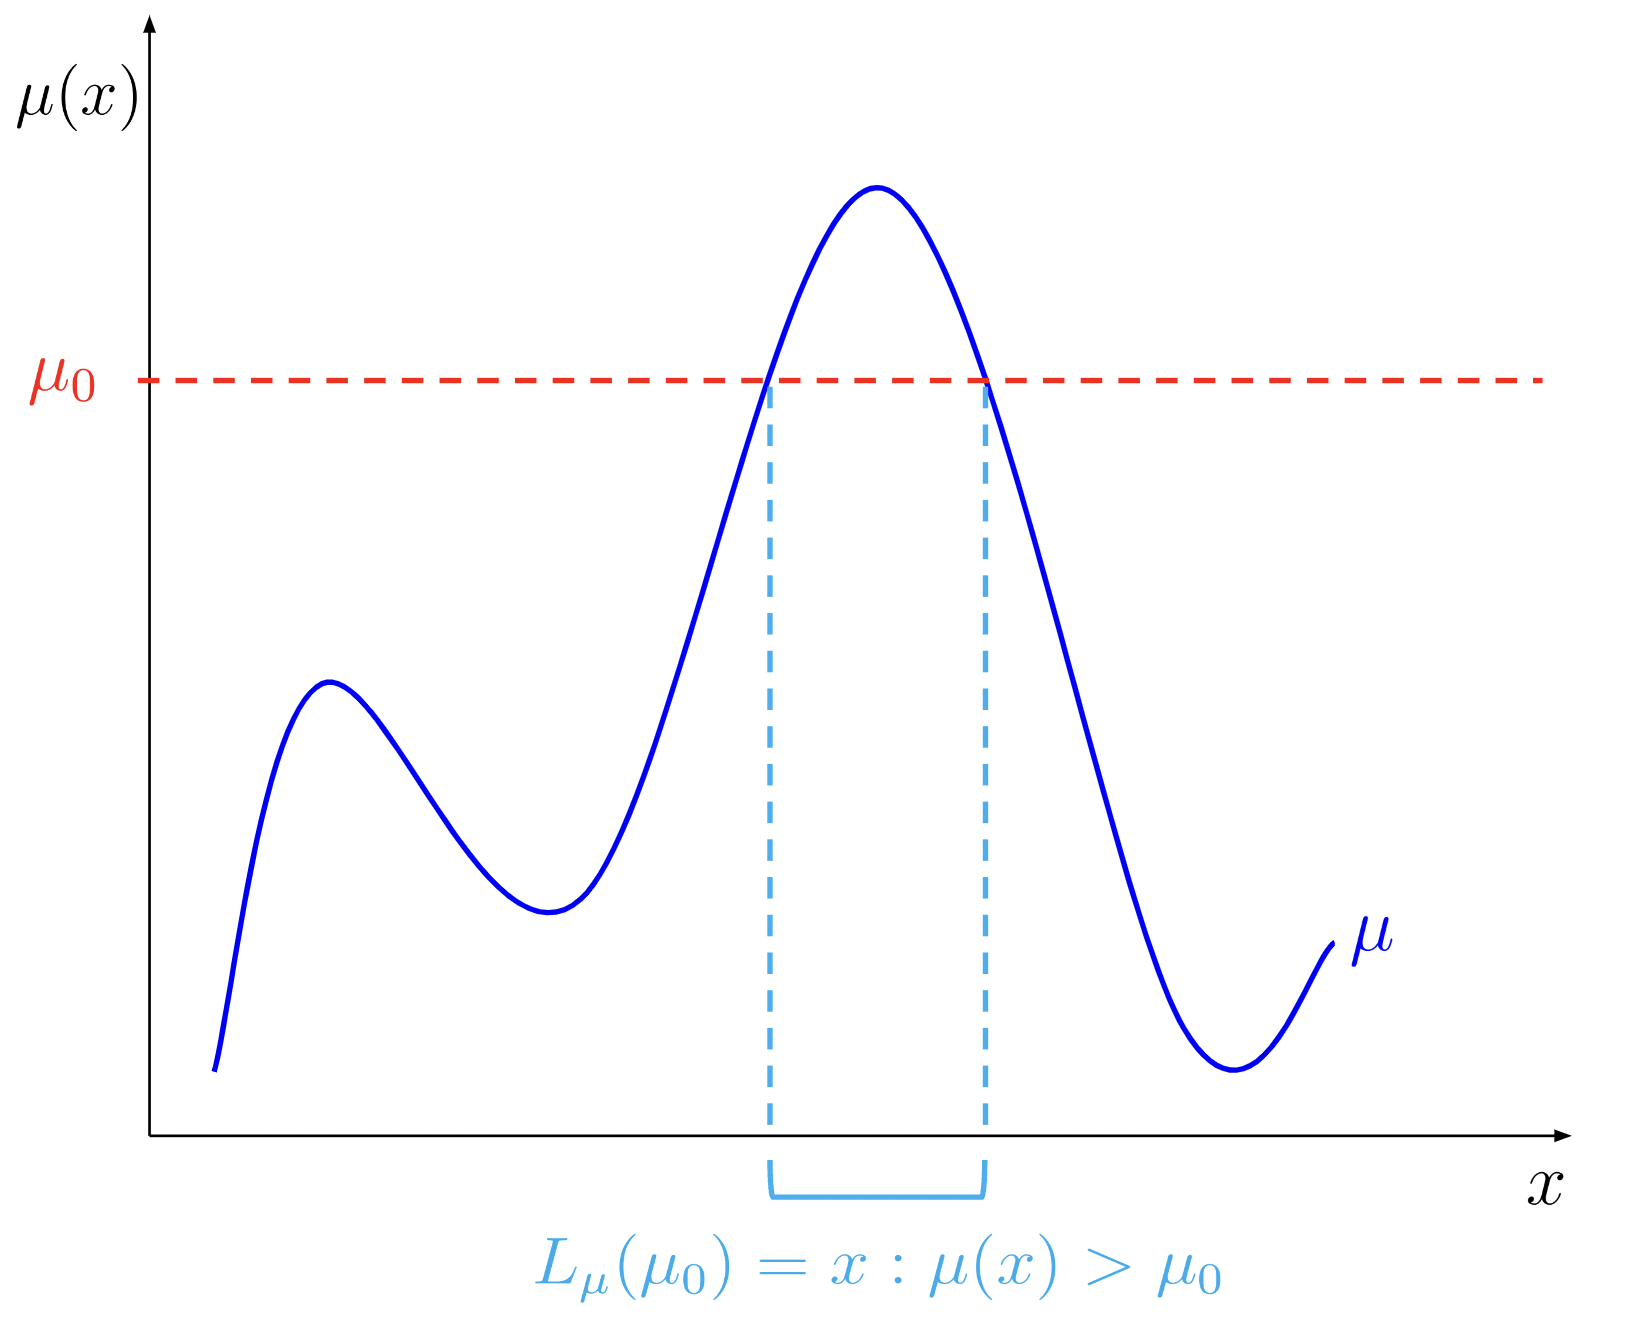
\includegraphics[width=0.7\textwidth]{/Users/ntb3/Desktop/Grad_Project/Thesis_Figures,Images,Tables/methodology_levelset.png}
	\caption{Level set of a measure $\mu$}
	\label{fig:level set}
	\end{figure}

 
 
 Let $f$ and $g$ be two measures. To compare measures $f$ and $g$, we can measure the level sets of one measure with respect to the other measure. The measure of the level set $L_f(c)$ with respect to $g$ is 
 
 \begin{equation} \label{eq:conditionallevelset}
 	I_{g|f}(c)=\int_{x_i \subset L_f(c)} g(x) dx
 \end{equation}
 
 	\begin{figure} [!htbp]
 	\centering
 	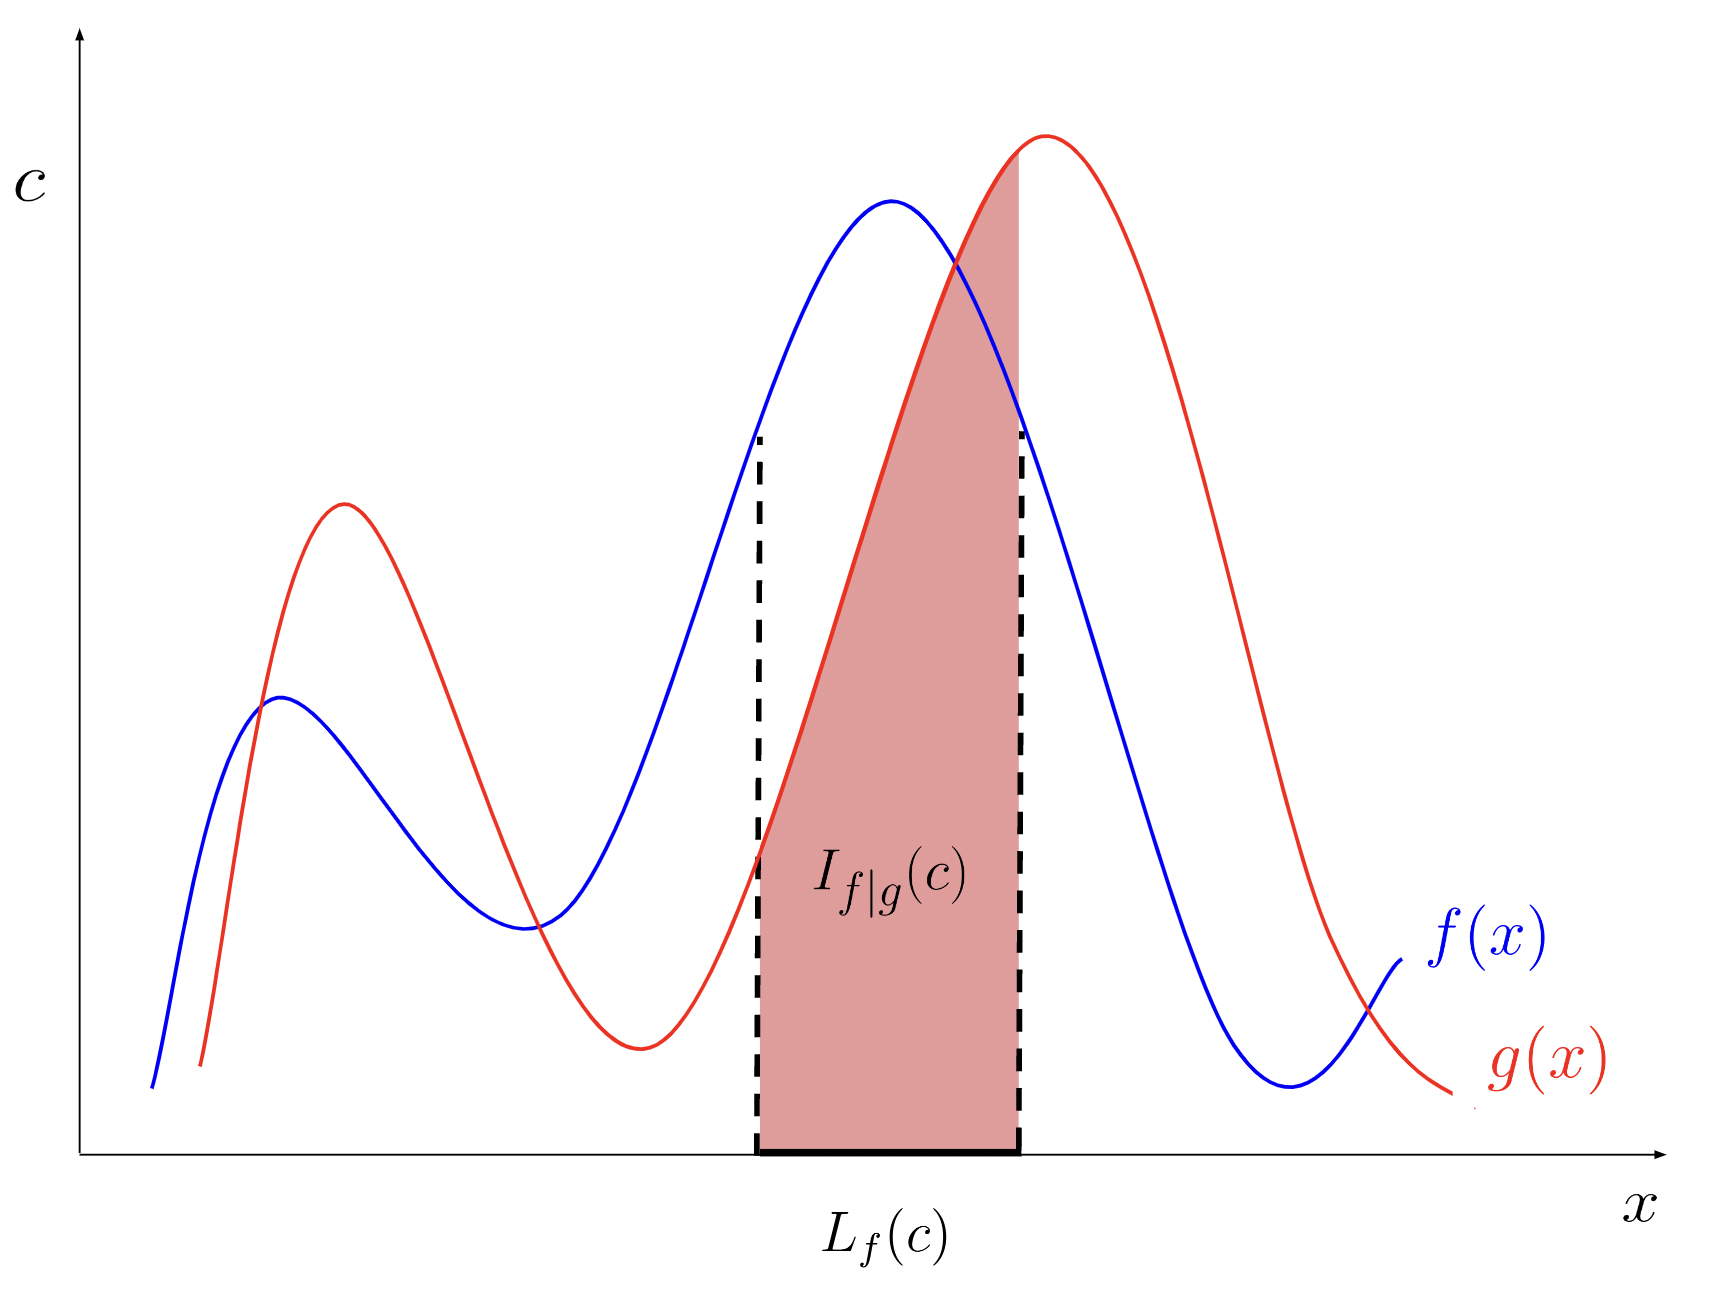
\includegraphics[width=0.7\textwidth]{/Users/ntb3/Desktop/Grad_Project/Thesis_Figures,Images,Tables/levelset_f|g.png}
 	\caption{Mass $I_{g|f}(c)$ of the level set $L_f(c)$ with respect to measure $g(x)$ equals the area of the shaded region. Measure $f(x)$ is shown by the blue line and measure $g(x)$ is shown by the red line.}
 	\label{fig:mass_of_level_sets}
 \end{figure}
 
 \subsubsection{Receiver Operating Characteristic (ROC)}
 To compare measures on intervals, the Receiver Operating Characteristic(ROC) can be used. To define the ROC consider three measures $f$, $g$ and $h$. The receiver operating characteristic of measure $h$ with respect to the ordered pair of measures $f$ and $g$, denoted by $R(f,g|h)$, is the set $(I_{f|h}(c),I_{g|h}(c))$ where parameter $c \geq 0$. Every level set $L_h(c)$ corresponds to a specific point in the set $R(f,g|h)$. The measure of the level set $L_h(c)$ corresponding to measures $f$ and $g$ is represented by the $x$ and $y$ coordinates of the point, respectively. The normalized (probability) measures used in this work adhere to the condition $f(X) = g(X) = h(X) = 1$. The following properties for the ROC can be inferred for normalized probability measures:
 
 - Any elements of $R(f,g|h)$ fall within the the two-dimensional unit square $[0,1] \times [0,1]$.
 
 - The points $(I_{f|h}(\infty), I_{g|h}(\infty)) = (0,0)$ and $(I_{f|h}(0), I_{g|h}(0)) = (1,1)$ are in the set $R(f,g|h)$.
 
 - The values of $R(g,g|f)$ lie on the line connecting the points $(0,0)$ and $(1,1)$.
 
 
  
 \begin{figure} [!htbp]
 	\centering
 	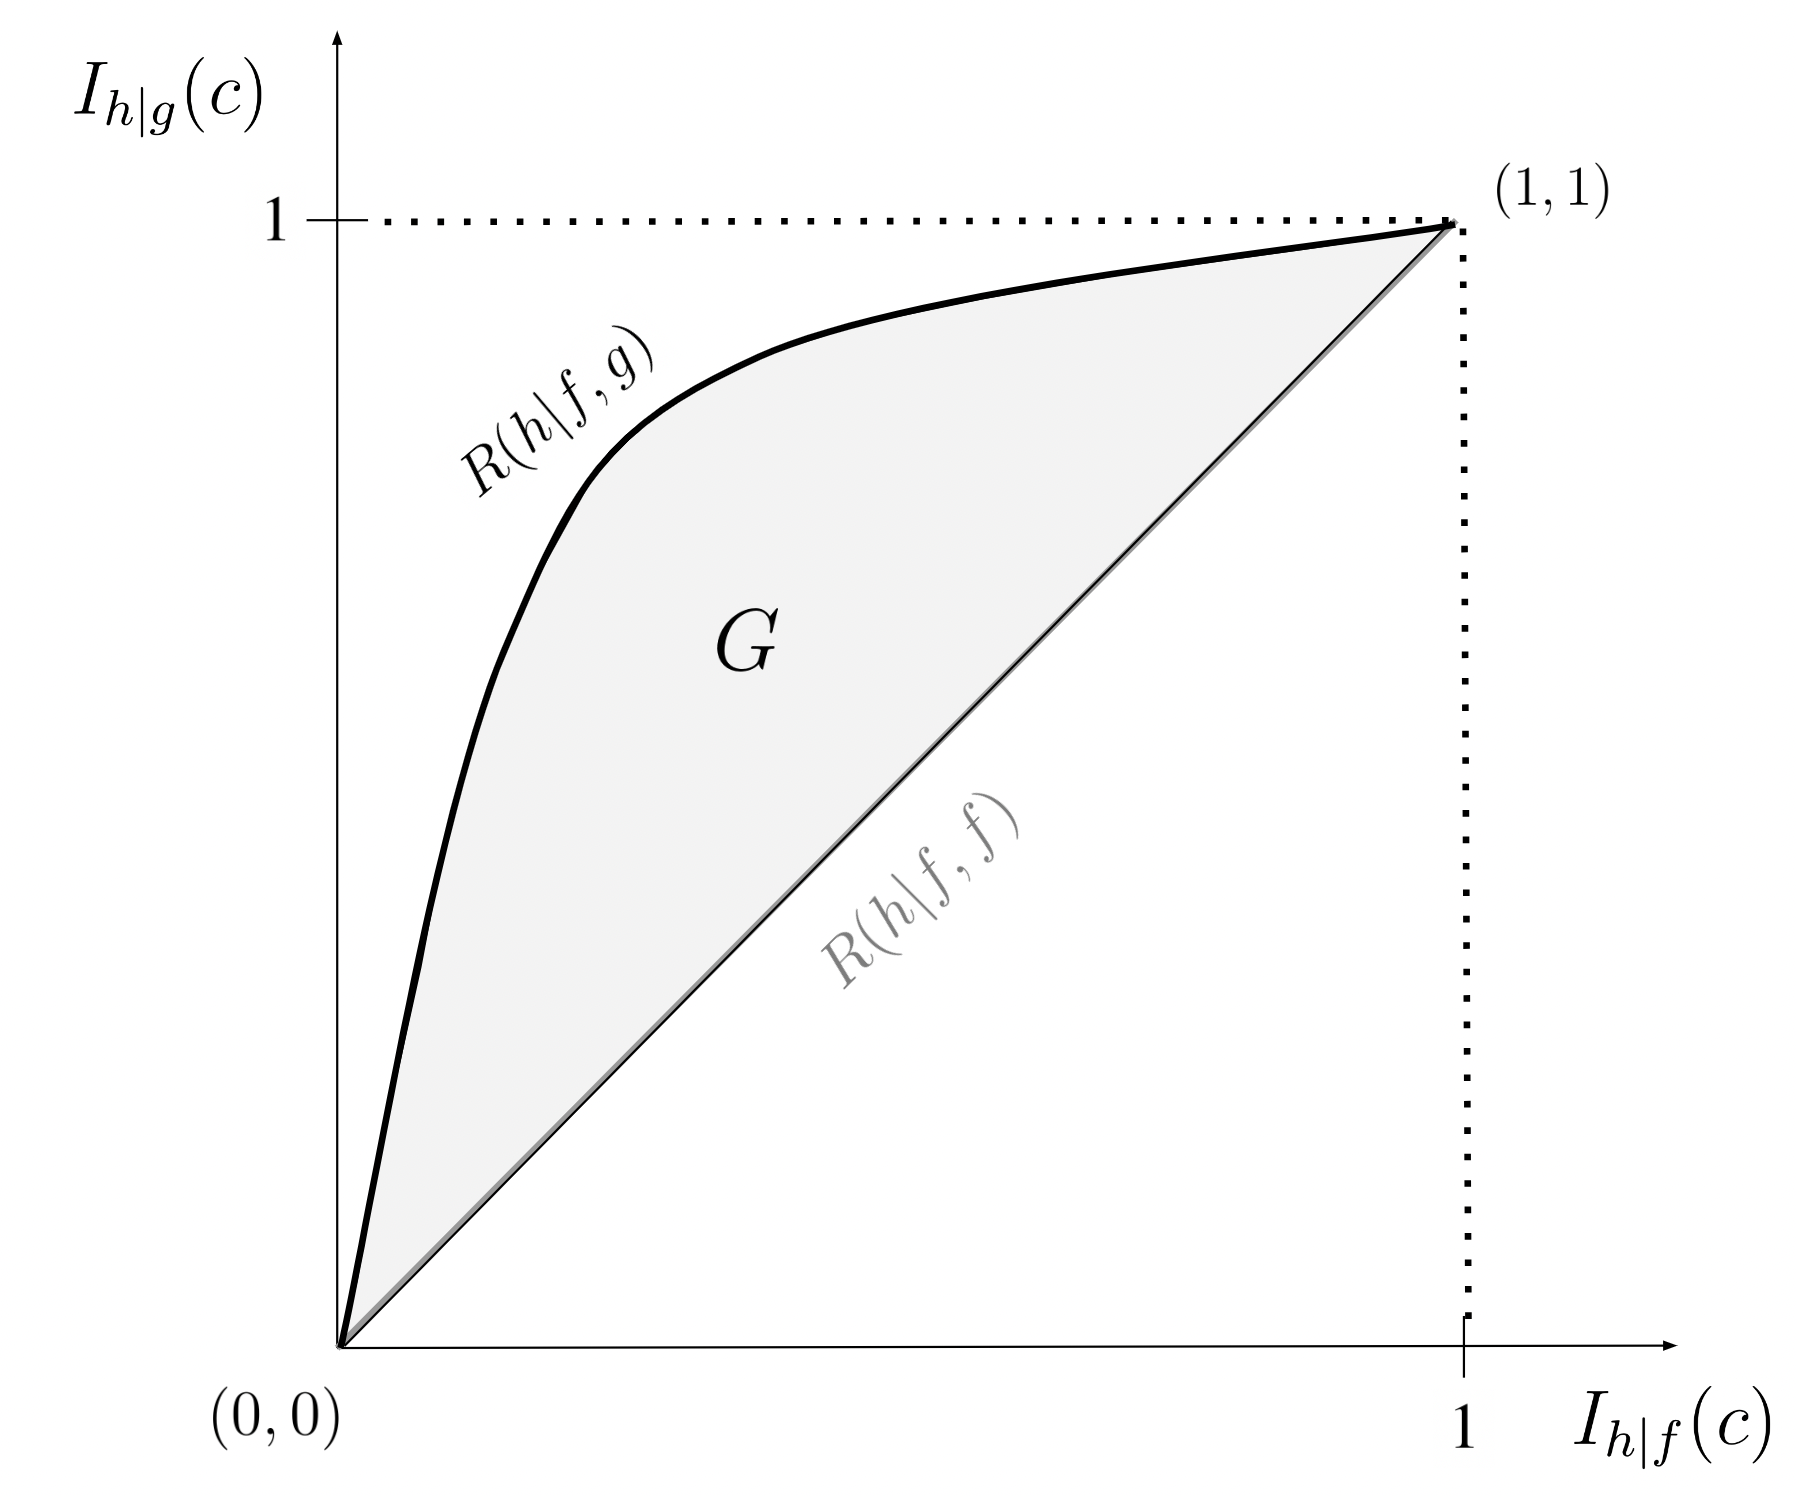
\includegraphics[width=0.7\textwidth]{ /Users/ntb3/Desktop/Grad_Project/Thesis_Figures,Images,Tables/methodology_ROC.png}
 	\caption{ROC diagram $R(f,g|h)$: a parametric plot of $I_{g|h}(c)$ vs $I_{f|h}(c)$ for $c \geq 0$. The set $R(f,f|h)$ always lies on the diagonal (grey).
 	}
 	\label{fig:mass_of_level_sets}
 \end{figure}
 

 
\subsubsection{Absolute Localization}
The ROC diagram can be used to compare measures on the same domain and quantifying the degree of concentration of a given measure. To quantify the degree of concentration of a measure, compare the measure to a uniform measure using the following properties.
 
For the uniform measure $U$ which assigns equal values to all subsets $x_i$, and any two measures $f$ and $g$:
 
 - The set $R(f,g|U)$ includes two points, namely (0,0) and (1,1).
 
 - The set $R(U,P|P)$ is situated on or above the diagonal line that connects points (0,0) and (1,1). 
 
 - If $f \neq U$ then $R(U,f|f)$ encompasses at least one point above the diagonal line. 
 
 %This feature arises from heterogeneities in P, where subsets Xi have a higher measure than other subsets, resulting in the accumulation of a greater value over the level sets of P when integrated with respect to P itself instead of with respect to U. 
 The absolute localization of measure $f$ can be quantified as the amount of deviation of $R(U,f|f)$ from the diagonal line 
 A point $(x,y)$ in the set $R(U,f|f)$ corresponds to a level set $L$ where $f(L) = y$ and $U(L) = x$. The point $(x,y)$ will be located close to the corner point $(0,1)$, far from the diagonal line, if a significant portion of $f$ is concentrated within a small region of $L$. 
 
 The Gini coefficient can be used to provide a precise measure of absolute localization. The Gini coefficient for absolute localization, denoted $G_f$, is twice the area between the curve of $R(U,f|f)$ and the diagonal line. $G_f$ can take on values between $0$ and $1$, where $G_f = 0$ indicates $f = U$, and $G_f$ gets closer to $1$ when $f$ becomes more heterogeneous (more localized). 
 
\subsubsection{Relative Localization} % 
 
 Relative localization is a measure of the localization of measure $f$ with respect to another non-uniform measure $g$. Relative localization means that measure $f$ is concentrated within the same domain as $g$ and it has more pronounced peaks(its measure of absolute localization is higher). This concepts is illustrated in Figure (INSERT REFERENCE NUMBER HERE) where $f$(red) is a more localized version of $g$(blue), $f$ has a larger absolute concentration than $g$ and is located within the same domain.
 
 To measure relative localization use the receiver operating characteristic for the set $R(f,g|g)$ with every point in the set corresponding to a particular level set $L_g(c)$. This set may include points below the diagonal line, indicating that the corresponding level sets of measure Q accumulate a higher mass with respect to measure P than with respect to Q itself. This situation is interpreted as relative localization of P with respect to Q. 
 
 To quantify the relative localization of measure $f$ with respect to measure $g$, we calculate the area above ROC curve $R(f,g|g)$, denoted as $G_{g|f}$. The parameter $G_{g|f}$ ranges from $0$ to $1$. If $G_{g|f} < \frac{1}{2}$ then measures $f$ and $g$ are not concentrated within the same regions. If $f$ is a localized version of $g$ then $G_{g|f} > \frac{1}{2}$ 
 

$I_{g|f}(c)$

\subsubsection{ROC and Random Variables}

A general measure can be changed into a probability measure. A probability measure is a function $P$ defined on a sigma-algebra $\Sigma$ of subsets of a sample space $S$, such that:

Non-negativity: For any set $A \in \Sigma, P(A) \leq 0$.

Normalization: $P(S) = 1$.

Countable additivity: For any sequence of disjoint sets $A_1, A_2, ..., A_n \in \Sigma$, the probability of their union is the sum of their individual probabilities:

$P(A_1 U A_2 U ... U A_n) = P(A_1) + P(A_2) + ... + P(A_n)$.

The sigma-algebra $\Sigma$ defines the collection of events for which probabilities can be assigned, and the axioms ensure that the probabilities are non-negative, normalized, and additive.

To change a measure $\mu$ to a probability measure $v$, you need to normalize the measure by dividing each set's measure by the measure of the entire space. This normalization ensures that the measure of the entire space is equal to 1. Define the new measure $v$ on $\Sigma$ as follows: 

\begin{equation}
	v(A) = \mu(A) / \mu(X)
\end{equation}
\noindent for all $A$ in $\Sigma$. $v$ must satisfy the properties of a measure: non-negativity, countable additivity, and $v(\emptyset) = 0$.

\subsubsection{Theoretical ROC for a Random Variable}

Let $X$ be a normalized random variable with probability density function(PDF) $f_X(x)$
and the cumulative distribution function (CDF) $F_X(x)$. The ROC diagram of $X$ with respect to a uniform random variable $U$, denoted $R(U,x|x)$ can be obtained by plotting $I_{X|X}(c)= P(x > c)$ on the x-axis and $I_{U|X}(c)=\int_{c}^{\infty} x f(x)dx$ on the y-axis. To obtain the theoretical ROC curve for the exponential random variable, the x-coordinates can be parameterized as follows:

\begin{equation} \label{eq:xcoord}
	x=P(X>c)=1-F(c)
\end{equation}

and the y-coordinates can be parameterized 

\begin{equation} \label{eq:ycoord}
	y= \int_{c}^{\infty} x f(x)dx
\end{equation}

The theoretical ROC curve for a random variable can sometimes be parameterized in terms of just $x$ and $y$ and will be a monotonically increasing curve that starts at $(0, 0)$ and ends at $(1, 1)$ with equation $R(U,X|X)$. The Gini coefficient for a random variable is thus:

\begin{equation} \label{eq:Gini}
	G = 2\int_0^1 R(U,X|X) -x  dx 
\end{equation}

\subsubsection{Theoretical ROC for an Exponential Random Variable}

 Let $X$ be a normalized exponential random variable with parameter $\lambda =1 $. The PDF of $X$ is 
 \begin{equation}
 f_X(x) = \left\{
 	 e^{- x}  \ \ \ \mbox{if } x \geq 0 
	\right\}
\end{equation}   

\noindent and the CDF for $X$ is 

 \begin{equation}
	F_X(x) = \left\{
		1- e^{- x}  \ \ \ \mbox{if } x \geq 0 
	\right\} .
\end{equation}  

The coordinates of the ROC curve can be parameterized as follows:

\begin{equation} \label{eq:xcoord_exp}
	x=e^{- c}
\end{equation}

\begin{equation} \label{eq:ycoord_exp}
	y = (c +1)e^{-c}
\end{equation}

Solving Equation (\ref{eq:xcoord_exp}) for $c$, yields

\begin{equation}
	c = ln(x)
\end{equation}

Substituting this in for $c$ in Equation (\ref{eq:ycoord_exp}) yields

\begin{equation}
	y =  -xlnx+x
\end{equation}

The theoretical ROC curve for an exponential random variable is therefore:

\begin{equation}
	R(U,X|X) = \left\{
		-xlnx+x \ \ \  \text{ for } 0 < x \leq 1 
\right\}
\end{equation}

  
\begin{figure} [!htbp]
	\centering
	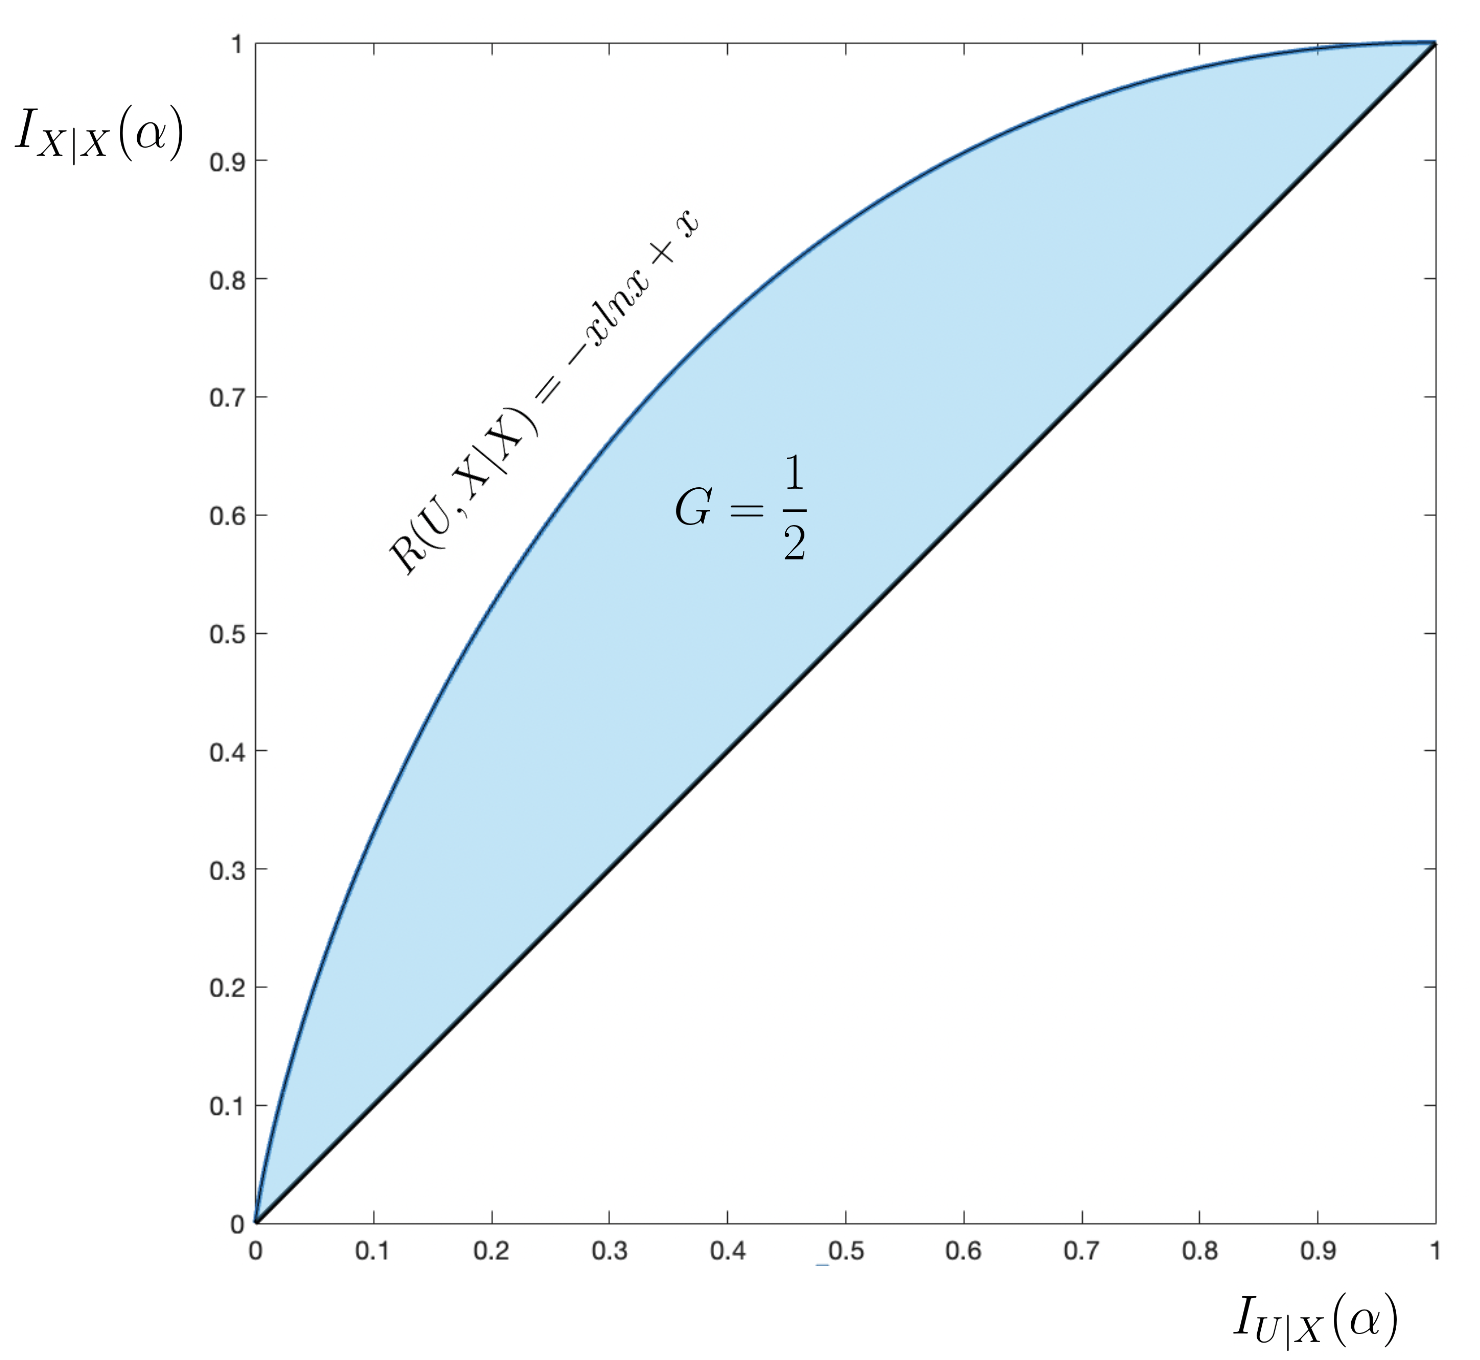
\includegraphics[width=0.7\textwidth]{ /Users/ntb3/Desktop/Grad_Project/Thesis_Figures,Images,Tables/Theoretical_Exponential_ROC.png}
	\caption{ROC diagram $R(U,X|X)$: a parametric plot of $I_{U|X}(c)$ vs $I_{X|X}(c)$ for $c \geq 0$. 
	}
	\label{fig:mass_of_level_sets}
\end{figure}

The Gini coefficient for an exponential variable is thus:

\begin{equation}
	G = 2\int_0^1 -xlnx dx = \frac{1}{2}
\end{equation}

\pagebreak

\clearpage

\subsubsection{Theoretical ROC for a Pareto Random Variable}

Let $X$ be a normalized pareto random variable with parameters $x_m =1$ and $\alpha \geq 1 $. The PDF of $X$ is 
\begin{equation}
	f_X(x) = 	\frac{\alpha x_m^{\alpha}}{x^{\alpha+1}}  , x \geq x_m, 
\end{equation}   

\noindent and CDF 

\begin{equation}
	F_X(x) = 	1- \left({\frac{x_m}{x}}\right)^{-\alpha} , x \geq x_m 
\end{equation}  

Normalizing this probability distribution by its mean $(E(x)=\frac{\alpha x_m}{\alpha-1})$ yields the following PDF and CDF

\begin{equation}
	f_X(x) = 	\frac{\alpha (\frac{\alpha - 1}{\alpha})^{\alpha}}{x^{\alpha+1}} 
\end{equation}   

\noindent and CDF 

\begin{equation}
F_X(x) = 1- \left({\frac{\alpha -1}{\alpha x}}\right)^{\alpha}
\end{equation}  


The x-coordinates of the ROC for a normalized pareto random variable can be parameterized as follows:

\begin{equation} \label{eq:xcoord_pareto}
	x= \left(\frac{\alpha -1}{\alpha c}\right)^{\alpha}
\end{equation}

and the y-coordinates can be parameterized 

\begin{equation} \label{eq:ycoord_pareto}
	y= \left( \frac{\alpha -1}{\alpha}\right) ^{\alpha -1} c^{1-\alpha}
\end{equation}

Solving Equation (\ref{eq:xcoord_pareto}) for $c$, yields

\begin{equation}
	c= \left( \frac{\alpha -1}{\alpha} \right) x^{-\frac{1}{\alpha}}
\end{equation}

Substituting this in for $c$ in Equation (\ref{eq:ycoord_pareto}) yields

\begin{equation}
	y = x^\frac{\alpha -1}{\alpha}
\end{equation}


The theoretical ROC curve for an Pareto random variable will therefore be a monotonically increasing curve that starts at $(0, 0)$ and ends at $(1, 1)$ and has equation:

\begin{equation}
	R(U,X|X) =  x^\frac{\alpha -1}{\alpha}, 0 < x \leq 1, \alpha >1
\end{equation}


The Gini coefficient for an Pareto variable is thus:

\begin{equation}
	G = 2\int_0^1  x^\frac{\alpha -1}{\alpha} -x dx = \frac{1}{2\alpha -1}
\end{equation}


\begin{figure} [!htbp]
	\centering
	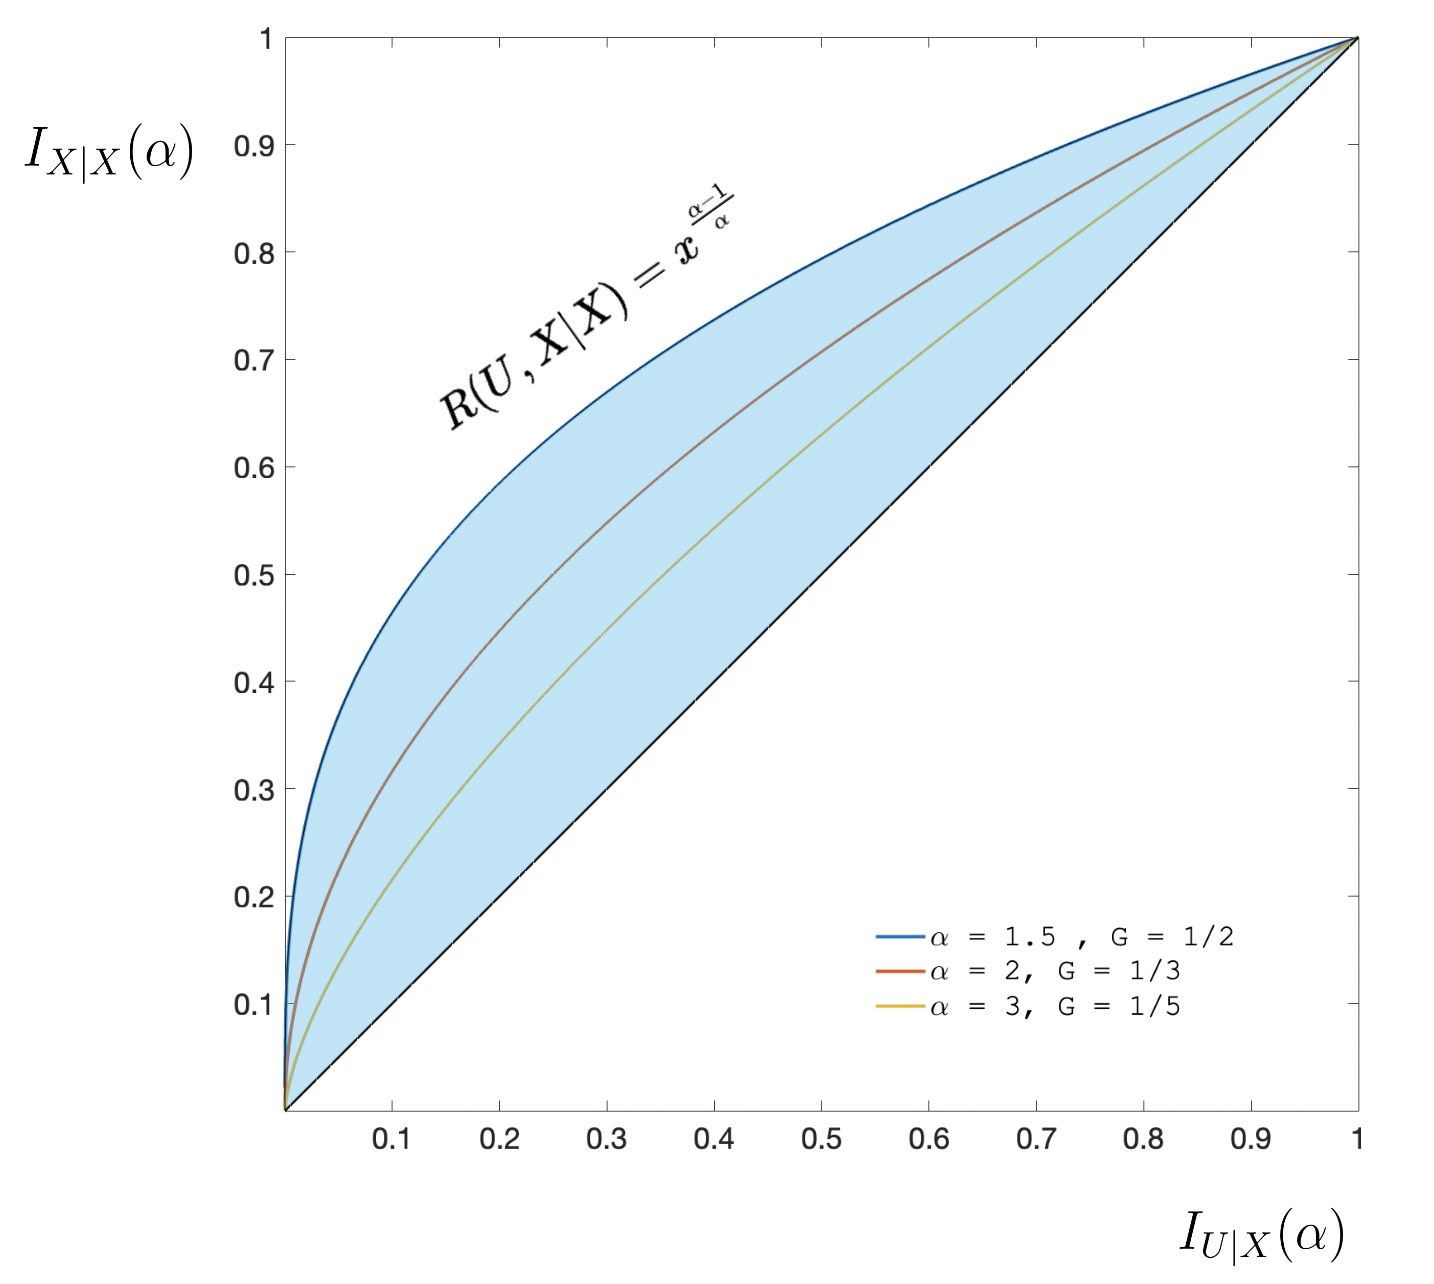
\includegraphics[width=0.7\textwidth]{ /Users/ntb3/Desktop/Grad_Project/Thesis_Figures,Images,Tables/Theoretical_Pareto_ROC.png}
	\caption{ROC diagram $R(U,X|X)$: a parametric plot of $I_{U|X}(c)$ vs $I_{X|X}(c)$ for $c \geq 0$ for a pareto random variable with parameter $\alpha = 3$.
	}
	\label{fig:mass_of_level_sets}
\end{figure}


\pagebreak


\subsubsection{Theoretical ROC for a Bivariate Random Variables}

\indent Let $X$ and $Y$ be continuous random variable with joint probability density function(PDF) $f_{X,Y}(x,y)$
and the cumulative distribution function (CDF) $F_{X,Y}(x,y)$. Consider a level set $L_X(x_0)$ corresponding to a threshold on the random variable $X$ such that $X>x_0$.

\begin{figure} [!htbp]
	\centering
	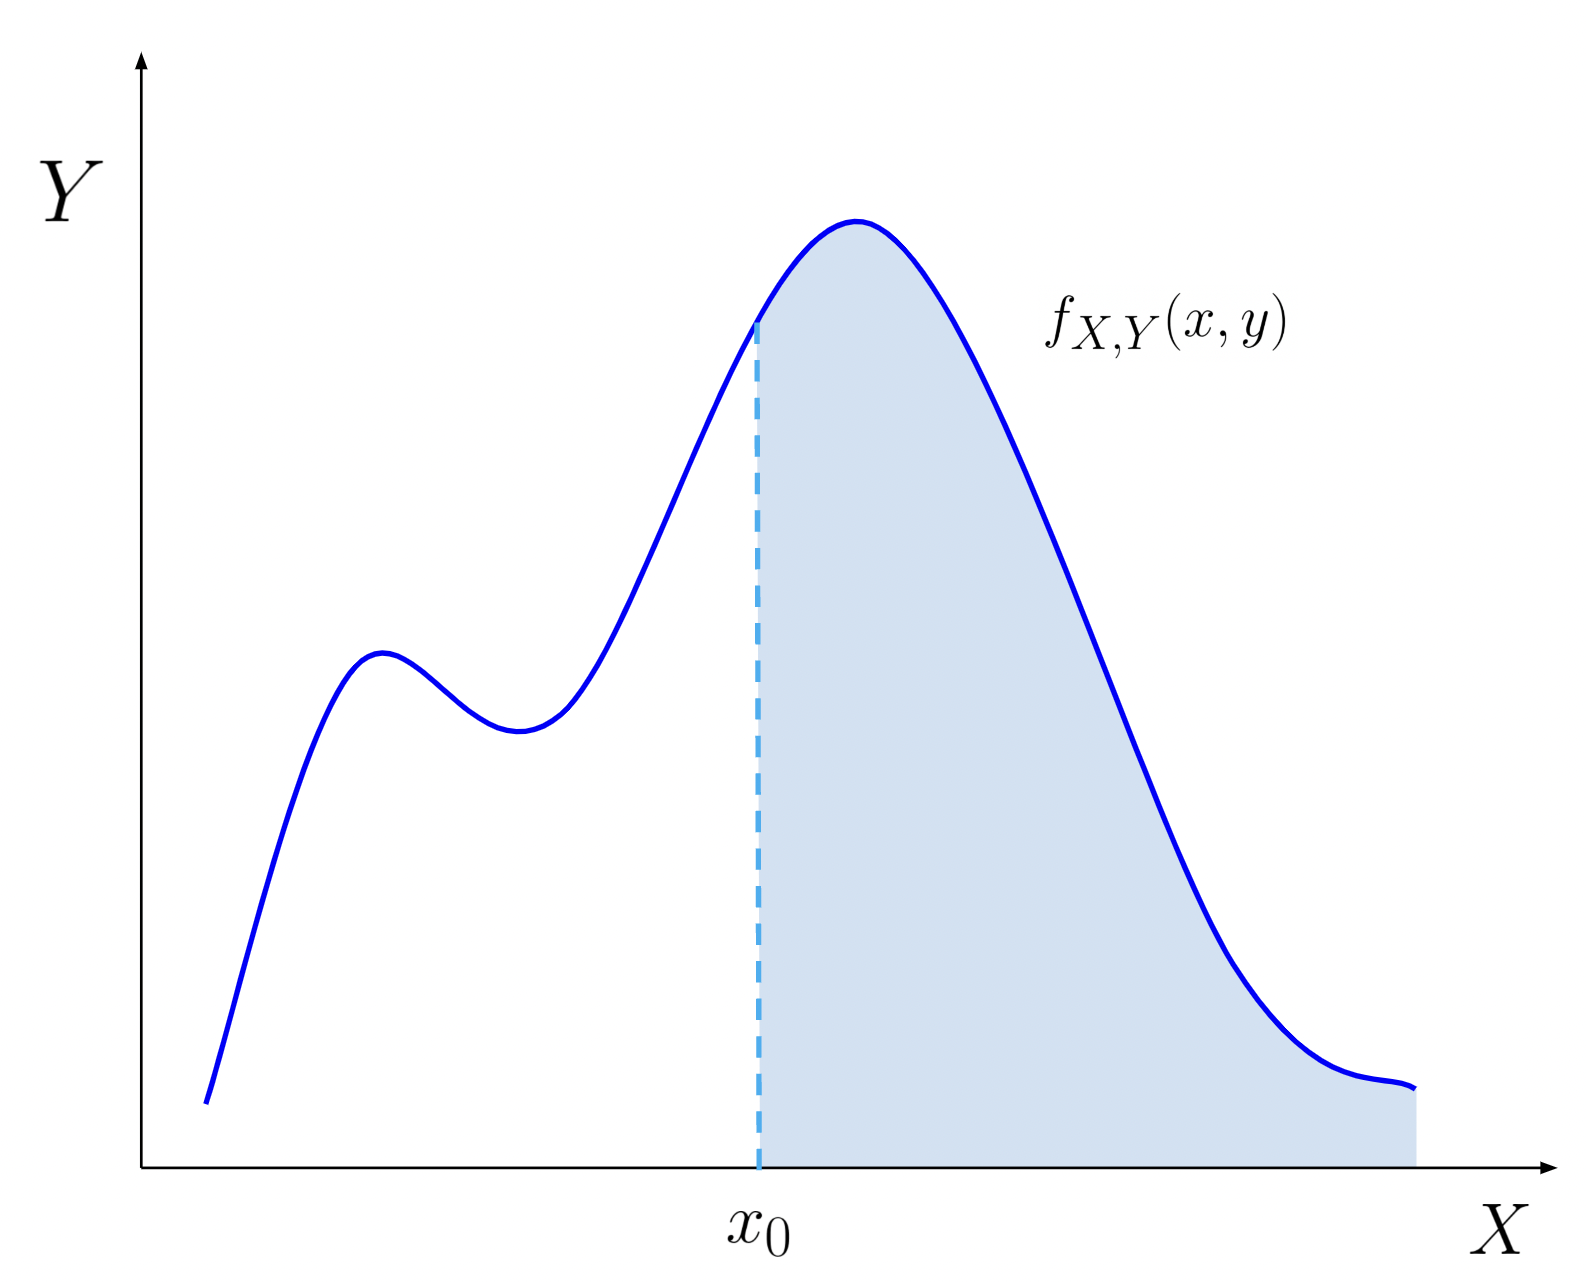
\includegraphics[width=0.7\textwidth]{ /Users/ntb3/Desktop/Grad_Project/Thesis_Figures,Images,Tables/methodology_levelset_bivariate.png}
	\caption{A level set $L_X(x_0)$ corresponding to a threshold on the random variable $X$ such that $X>x_0$.
	}
	\label{fig:bivariate_levelset}
\end{figure}


The ROC diagram of $(X,Y)$ with respect to $X$, denoted $R(X,Y|X)$. To obtain the theoretical ROC curve for a random variable, the x-coordinates can be parameterized as follows:

\begin{equation} \label{eq:xcoord_bivariate}
	x=I_{Y|X}(x_0)= \int_{x_0}^{\infty}\int_{-\infty}^{\infty} y f_{X,Y}(x,y)dy dx
\end{equation}

and the y-coordinates can be parameterized 

\begin{equation} \label{eq:ycoord_bivariate}
	y= I_{X|X}(x_0)=\int_{-\infty}^{\infty}\int_{x_0}^{\infty} x f_{X,Y}(x,y)dx dy
\end{equation}

Like the theoretical ROC curve for a random variable, the ROC for a two random variables can sometimes be parameterized in terms of just $x$ and $y$ and will be a monotonically increasing curve that starts at $(0, 0)$ and ends at $(1, 1)$ with equation $R(U,X|X)$. The Gini coefficient will be defined by Equation (\ref{eq:Gini}).

\subsubsection{Theoretical ROC for a Bivariate Exponential Random Variables}

Let $X$ and $Y$ be two independent exponential random variable with parameter $\lambda_1$ and $\lambda_2$. The probability density function's(p.d.f) of $X$ and $Y$ are of the form
\begin{equation}
	f(x) = \lambda e^{-\lambda x}, \ \ \  x \geq 0.
\end{equation}

with joint density function
\begin{equation}
	f_{X,Y}(x,y) = f(x) \cdot f(y)= \lambda_1  e^{-\lambda_1x}\lambda_2 e^{-\lambda_2 y}, \ \ \ x \geq 0,  y \geq 0.
\end{equation}


\section{Results - Quantifying Space-time Clustering on a Given Fault Network }

\label{sec:res}

The above methodology can be used as a novel statistical approach to quantify regional earthquake clustering. Clustering was introduced in the background section as a fundamental component of understanding seismicity and earthquake triggering mechanisms. Using the ROC diagram to measure space-time clustering allows disentangling effects related to concentration of events around a heterogeneous regional fault network from coupled space-time fluctuations. 

In this section the ROC will be used to examine and illustrate seismic clustering in multiple seismically active regions, including the Reno area. The ROC will be used to explore several general measures of seismic rate that can account for the number of events, the total area of faultbreaks, seismic moment, and more. Systematically examine general and coupled space-time clustering of raw and declustered catalogs. The Gini coefficeint will be presented as a simple and robust measure of space-time clustering to illustrate and quantify earthquake clustering with examples of seismicity from regions worldwide.


\subsection{Data}
​​
For this study, the ANSS Comprehensive Earthquake Catalog was used. The regions examined for this study are Reno, southern California, Japan, New Zealand, Italy, the Atlantic and Pacific. Specifics of the analysis for each region are in the table below.



\begin{figure} [!htbp]
	\centering
	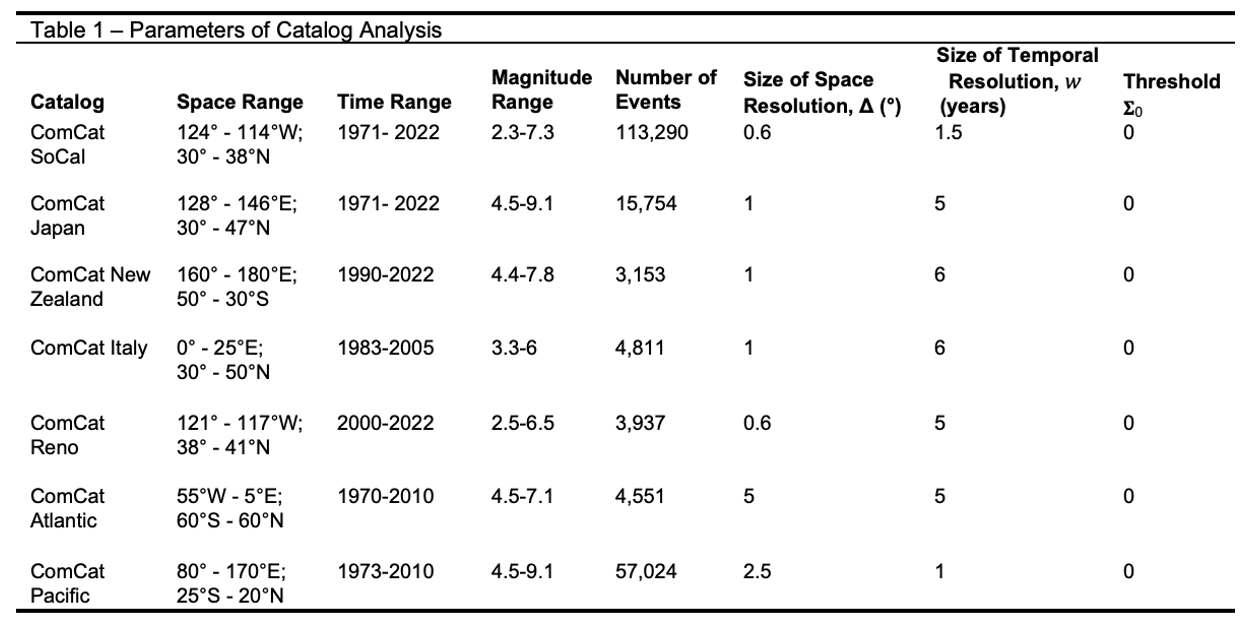
\includegraphics[width=1.0\textwidth]{ /Users/ntb3/Desktop/Grad_Project/Thesis_Figures,Images,Tables/data_description_table.png}
	\caption{Table 1 NEEDS A CAPTION	}
	\label{fig:data_table}
\end{figure}


\subsection{Methodology}
Receiver operating characteristic diagrams (ROC for short) were used to assess the inhomogeneity of the space-time distribution of seismicity in the regions of this study in a systematic way. These ROC diagrams were used to produce a single measure of space-time clustering, the Gini coefficient ($G$) which is an efficient and stable measurement of earthquake clustering.

The coefficient $G$ may assume values between $0$ and $1$. A value of $G$ close to $1$ indicates a large portion of events are concentrated in a small fraction of the examined space-time volume.

More formally, we partition the examined space-time area into voxels with space dimension $\delta$ and time size w, and measure seismic activity within a voxel centered at location $x$ at time $t$ by the equation here where the summation is taken over all events within the voxel, $\beta$ is a parameter we change to understand the different characteristics of clustering in that region, and M is the event magnitude. $\beta = 0$ corresponds to counting events, $\beta = 1$ approximates the faultbreak area, and $\beta = \frac{3}{2}$ corresponds to the seismic moment. We only examine voxels with the time-integrated value of $\Sigma$ being larger than a threshold $\Sigma_0$ (in this work, $\Sigma_0 = 0$). 

Figure 3 illustrates the general procedure for quantifying clustering of earthquakes in southern California with the (ROC) diagram.

First, we evaluate the general clustering. Here, the ROC diagram is a plot of $\Sigma$ within the most active voxels ($y$-axis) vs. the fraction of the examined non-empty voxels ($x$-axis). 

Next, in order to remove the effects of marginal space and time heterogeneities in the examined catalog, we evaluate coupled space-time clustering. In this analysis, the ROC diagram is a plot of sigma within the most active voxels (y-axis) vs. the weighted fraction of the examined non-empty voxels. The weights are determined by the factorized space-time rates of background events. Declustering is done by the method of Zaliapin and Ben-Zion.

Example of Analysis for southern California
Figure 4 shows an example of this analysis for Southern California . 

The first plot is a measure of earthquake clustering with respect to a uniform measure. The red shading corresponds to the most active voxels in our region over the period of time for the catalog. Clearly seismicity in the southern califronia area is not uniform over the region. instead, a large fraction of earthquakes occurs in a relatively small time-space volume. We call this "clustering" and measure it by a general Gini coefficient.


This general clustering is attributed to two reasons: 1st, earthquakes occur along fault zones (see Fig. 1). 2nd, there exist groups of events highly localized in a given area during a short time (these would be aftershock sequences after a large earthquake).



We would like to separate these two effects. Technically, this is done
by introducing space-time coupling Gini coefficient.



In other words, we start by using a measure that shows no clustering if events occur uniformly in space and time. Then we introduce a more delicate measure that doesn't include clustering related to events around hot spot areas that are active all the time, or burst of activity in time that might affect an entire region. Then we measure how strongly the observed clustering deviates from this new (factorized) model.  All deviations represent burst of activity that are localized in time and space.

\subsection{Results}

An interesting observation is that this coupled clustering (the red measure) is rather strong, and varies substantially from catalog to catalog.


The results displayed in Figure 6 show the gini coefficients G for all regions for $\beta = 0$.  
An interesting observation is that this coupled clustering is (a) rather strong, and (b) varies substantially from catalog to catalog. For the other measures, clustering for all events, for background events and coupled space time clustering for background events (the blue yellow and green measures in the figures) we see a more uniform clustering over all regions. The gini coefficient for coupled space-time clustering for all events can help us identify regional differences in clustering because there is the greatest variability in this measure.
By the way, we found that the region with the largest clustering was Reno, NV.

\subsection{Conclusions}
Some general conclusions from my work are that the overall observed earthquake clustering is high for both the raw catalog and declustered catalog.
•The marginal space clustering (fault network) plays a dominant role in the overall clustering
•When focusing on the coupled space-time clustering, different catalogs show different degrees of clustering, reflecting a variety of specific triggering conditions and mechanisms.
•Coupled clustering of declustered catalogs (for $\beta = 0$) is negligible ($G < 0.1$)



The main take away I hope you get from my presentation today is  that the gini coefficient for Coupled space-time clustering can be used as a metric that shows variability in clustering region to region. 











	
	\section{Discussion}
	\label{sec:discuss}
	
	\appendix
	\section{Title of Appendix A}
	
	%%%%%%%%%%%%%%
	% REFERENCES % using APA 7th edition
	%%%%%%%%%%%%%%
	\newpage
	\begin{thebibliography}{99}  %%%%%%%%%%%%%%%%%%%%%%%%%%%%%%%%%%%%%%%%%%%%%%%%%

		\bibitem{BP04}
		Baiesi, M. \& Paczuski, M., 2004. Scale-free networks of earthquakes and aftershocks, Phys. Rev. E, 69, 066106, doi:10.1103/PhysRevE.69.066106.
		
		\bibitem{B88}
		Brillinger, D. (1988), Some Statistical Methods for Random Process Data from Seismology and Neurophysiology, The 1983 Wold Memorial Lectures, Ann. Statist. 16, 1–54.
		
		\bibitem{BLR08}
		Bird, P., Liu, Z. \& Rucker, W.K., 2008. Stresses that drive the plates from below: definitions, computational path, model optimization, and error analysis, J. geophys. Res., 113, B11406, doi:10.1029/2007JB005460.
		
		\bibitem{DV72}
		Daley, D. J., \& Vere-Jones, D., A summary of the theory of point processes. In Stochastic Point Processes: Statistical Analysis, Theory and Applications (ed. Lewis, P. A. W.) (Wiley, New York
		1972).
		
		\bibitem{GR54}
		Gutenberg B. \& Richter C. (1954). Seismicity of the earth and associated phenomena (Second). Princeton University Press.
		
		\bibitem{HYS12}
		Hauksson, E., Yang W.,  \& Shearer P.M. , "Waveform Relocated Earthquake Catalog for Southern California (1981 to 2011)"; Bull. Seismol. Soc. Am., Vol. 102, No. 5, pp.2239-2244, October 2012, doi: 10.1785/0120120010
		
		\bibitem{KBZ21}
		Kato, A., and Y. Ben-Zion. (2021) 
		The generation of large earth- quakes, Nat. Rev. Earth Environ. 2, 26–39, doi: 10.1038/s43017- 020-00108-w.
		
		\bibitem{KBK14}
		Kreemer, C., Blewitt, G. \& Klein, E.C., 2014. A geodetic plate motion and global strain rate model, Geochem., Geophys., Geosyst., 15(10), 3849– 3889.
		
		\bibitem{O85}
		Ogata, Y. (1985), Statistical Models for Earthquake Occurrences and Residual Analysis for Point Processes, Research Memo. (Technical report), No. 288, Inst. Statist. Math., Tokyo.
		
		\bibitem{O88}
		Ogata, Y. (1988), Statistical Models for Earthquake Occurrences and Residual Analysis for Point Processes, J. Amer. Statist. Assoc. 83, 9–27.
		
		\bibitem{O99}
		Ogata, Y., 1999. Seismicity analysis through point-process modeling: a
		review, Seismicity Patterns, their Statistical Significance and Physical Meaning, pp. Wyss, M., Shimazaki, K. \& Ito, A., 471–507, doi.org/10.1007/978-3-0348-8677-2 14.
		
		\bibitem{UG97}
		Utsu, T., and Ogata, Y. (1997), Statistical analysis of seismicity. In Algorithms for Earthquake Statistics and Prediction, IASPEI Software Library 6, 13-94, International Association of Seismology and Physics of the Earth’s Interior in collaboration with the Seismological Society of America.
		
		\bibitem{ZGKH08}
		Zaliapin, I., Gabrielov, A., Keilis-Borok, V., \& Wong, H. (2008) 
		Clustering analysis of seismicity and aftershock identification. 
		{\em Physical Review Letters}, 101(1), 018501.
		
		\bibitem{ZBZ13a}
		Zaliapin, I., \& Ben-Zion, Y. (2013) 
		Earthquake clusters in southern California I: Identification and stability. 
		{\em Journal of Geophysical Research: Solid Earth}, 118(6), 2847--2864.

		\bibitem{ZBZ15}
		Zaliapin,I.\& Ben-Zion,Y.,2015.
		Artifacts of earth quake location errors and short-term incompleteness on seismicity clusters in southern California,
		Geophys. J. Int., 202 1949–1968.
		
		\bibitem{ZBZ16a}
		Zaliapin, I. \& Ben-Zion, Y. (2016) 
		Discriminating characteristics of tectonic
		and human-induced seismicity, Bull. seism. Soc. Am., in press.
		
		\bibitem{ZBZ16b}
		Zaliapin, I., \& Ben-Zion, Y. (2016)
		A global classification and characterization of earthquake clusters. 
		{\em Geophysical Journal International}, 207(1), 608--634.
	
		
		\bibitem{ZBZ21}
		Zaliapin, I., and Y. Ben-Zion (2021)
		Perspectives on Clustering and Declustering of Earthquakes 
		{\em Seismological Research Letters 2021}, 386–401, doi: 10.1785/0220210127.

		\bibitem{KZBZ22}
		Yevgeniy Kovchegov, Ilya Zaliapin, Yehuda Ben-Zion, Invariant Galton–Watson branching process for earthquake occurrence, Geophysical Journal International, Volume 231, Issue 1, October 2022, Pages 567–583, https://doi.org/10.1093/gji/ggac204
		
	
	\end{thebibliography}
	
	
	
\end{document}
